\documentclass[10pt,oneside,onecolumn,openany,final]{memoir}
\setstocksize{11in}{8.5in}

\usepackage[toc,lot,lof]{multitoc}
\usepackage[top=.5in, bottom=.5in, left=.75in, right=.75in]{geometry}
\usepackage{graphicx} \graphicspath{{./images/}}
\usepackage{longtable}
\usepackage{mdwlist}
\usepackage{microtype} \DisableLigatures{encoding = *, family = *}
\usepackage{multicol}
\usepackage{textcomp}
\usepackage[normalem]{ulem}
\usepackage{wrapfig}
\usepackage{xtab}
\usepackage{enumerate}
\usepackage{phonetic}
\usepackage{bbding}
\usepackage{linearb}
\usepackage{cypriot}
\usepackage{tipa}
\usepackage{xfrac}
\usepackage{appendix}
\usepackage{xparse}
\usepackage{letltxmacro}
\usepackage{makeidx} \makeindex
\usepackage[table,dvipsnames]{xcolor}
\definecolor{offyellow}{RGB}{255,255,128}
\definecolor{links}{RGB}{200,0,50}
\usepackage{placeins}
\usepackage{floatflt}
\usepackage{anyfontsize}
\usepackage{colortbl}
\usepackage{tabularx}
\usepackage{mdframed}
\usepackage{longtable}
\usepackage{tabu}
\usepackage{afterpage}

\usepackage{caption}

%% Font
\usepackage[T1]{fontenc}
\usepackage[bitstream-charter]{mathdesign}
\usepackage{aurical}

\usepackage[colorlinks=true,linkcolor=blue,urlcolor=links,pdfstartview={XYZ null null 1.00},bookmarksdepth=2]{hyperref}
%%%%%%%%%%%%%%%%%%%%%%%%%
%%%% End of Import tion %%%%%%%%%%%
%%%%%%%%%%%%%%%%%%%%%%%%%

%%%%%%%%%%%%%%%%%%%%%%%%%%%%%%%%%%%%%%%%%%%%%%%%%%
%%%%%%%%%%%%%%%%%%%%%%%%%%%%%%%%%%%%%%%%%%%%%%%%%%
%%% Revised Commands
%%%%%%%%%%%%%%%%%%%%%%%%%%%%%%%%%%%%%%%%%%%%%%%%%%
%%%%%%%%%%%%%%%%%%%%%%%%%%%%%%%%%%%%%%%%%%%%%%%%%%
\makeatletter

%fiddles with how chapter titles are displayed
\renewcommand{\@makechapterhead}[1]{%
\vspace*{0 pt}{%
\raggedright \normalfont \fontsize{32}{32} \selectfont \bfseries%
\ifnum \value{secnumdepth}>-1%
  \if@mainmatter \vspace{-8pt} {\fontsize{20}{20} \selectfont Chapter \thechapter:}\\[8pt]%
  \fi%
\fi
\hspace{0.65cm} #1\par\nobreak\vspace{20 pt}%
}}

%makes paragraphs show up closer together
\renewcommand{\paragraph}{%
\@startsection{paragraph}{4}%
{\z@}{1.0ex \@plus 1ex \@minus 0.2ex}{-1em} % wtf is an 'ex' anyways?
{\normalfont\normalsize\bfseries}%
}

%lets multicolumn have the proper background colors as defined by rowcolors
\let\oldmc\multicolumn
\newcommand{\mcinherit}{% Activate \multicolumn inheritance
  \renewcommand{\multicolumn}[3]{%
    \oldmc{##1}{##2}{\ifodd\rownum \@oddrowcolor\else\@evenrowcolor\fi ##3}%
  }}

\makeatother

%add labels within sections, subsections, and subsubsections
\LetLtxMacro{\oldsection}{\section}
\renewcommand{\section}[1]{\oldsection{#1}\label{sec:#1}}

\LetLtxMacro{\oldsubsection}{\subsection}
\renewcommand{\subsection}[1]{\oldsubsection{#1}\label{sec:#1}}

\LetLtxMacro{\oldsubsubsection}{\subsubsection}
\renewcommand{\subsubsection}[1]{\oldsubsubsection{#1}\label{sec:#1}}

%only put chapters and sections into the TOC
\setcounter{secnumdepth}{1}
%makes a subsubsection start off indented.
\setlength{\beforesubsubsecskip}{-\beforesubsubsecskip}

%%%%%%%%%%%%%%%%%%%%%%%%%%%%%%%%%%%%%%%%%%%%%%%%%%
%%%%%%%%%%%%%%%%%%%%%%%%%%%%%%%%%%%%%%%%%%%%%%%%%%
%%% Table Formatting
%%%%%%%%%%%%%%%%%%%%%%%%%%%%%%%%%%%%%%%%%%%%%%%%%%
%%%%%%%%%%%%%%%%%%%%%%%%%%%%%%%%%%%%%%%%%%%%%%%%%%
\newcolumntype{L}[1]{>{\raggedright\let\newline\\\arraybackslash\hspace{0pt}}m{#1}} %New type of column 'L' that is ragged-right, behaves like a paragraph, and allows manual definition of width like a 'p' column.
\newcolumntype{C}[1]{>{\centering\let\newline\\\arraybackslash\hspace{0pt}}m{#1}}  %New type of column 'C' that is centered, behaves like a paragraph, and allows manual definition of width like a 'p' column.
\newcolumntype{R}[1]{>{\raggedleft\let\newline\\\arraybackslash\hspace{0pt}}m{#1}}  %New type of column 'R' that is ragged-left, behaves like a paragraph, and allows manual definition of width like a 'p' column.
\newcommand{\header}{\rowcolor{headercolor}}
%when inserted in a row, makes that row the color headercolor

%%%%%%%%%%%%%%%%%%%%%%%%%%%%%%%%%%%%%%%%%%%%%%%%%%
%%%%%%%%%%%%%%%%%%%%%%%%%%%%%%%%%%%%%%%%%%%%%%%%%%
%%% New Commands
%%%%%%%%%%%%%%%%%%%%%%%%%%%%%%%%%%%%%%%%%%%%%%%%%%
%%%%%%%%%%%%%%%%%%%%%%%%%%%%%%%%%%%%%%%%%%%%%%%%%%

%%%%%%%%%%%%%%%%%%%%%%%%
%%Basic Formatting
%%%%%%%%%%%%%%%%%%%%%%%%
\newcommand{\originallineskip}{\baselineskip}
 %A command that is equal to the original \baselineskip of the doc, in case we change it for a section and want to change it back later
\newcommand{\ability}[2]{\smallskip
 \textbf{#1} #2} 
%The \ability{#1}{#2} command from legacy-source. Should rarely be directly used, changes to this will cascade into other new commands that use its functionality
\newcommand{\shortability}[2]{\noindent\textbf{#1} #2\\}
%A specialized version of the \ability command
\newcommand{\itemspace}{\setlength{\itemsep}{-1mm}\setlength{\topsep}{-1mm} }
%A command from legacy-source for compatabilty
\newcommand{\listone}{\begin{list}{$\bullet$}{\itemspace}}
\newcommand{\listtwo}{\begin{list}{$\triangleright$}{\itemspace}}
%A type of list from legacy sorce
\newcommand{\listnum}{\begin{list}{\textbf{\arabic{counter}}:}{\usecounter{counter}}}
\newcommand{\spell}[1]{\emph{\MakeLowercase{#1}}}
%makes spell name lowercase italics.
\setlength{\parindent}{0pt}

\newcommand{\half}[0]{\ensuremath{\sfrac{1}{2}} }
\newcommand{\third}[0]{\ensuremath{\sfrac{1}{3}} }
\newcommand{\fourth}[0]{\ensuremath{\sfrac{1}{4}} }

%%%%%%%%%%%%%%%%%%%%%%%%
%%Logic
%%%%%%%%%%%%%%%%%%%%%%%%
\newcommand{\testempty}{\empty}
\newcommand{\isempty}{\empty}
%Two commands that can be compared to one another for \ifx logic tests. \isempty should never be changed. If \testempty holds a value of anything but empty, the test should return false.
\newcounter{counter}

%%%%%%%%%%%%%%%%%%%%%%%%
%%Colors
%%%%%%%%%%%%%%%%%%%%%%%%
\colorlet{colorone}{white}
\colorlet{colortwo}{gray!15}
\colorlet{headercolor}{gray!50}
\colorlet{tablecolorone}{gray!40}
\colorlet{tablecolortwo}{gray!20}

%%%%%%%%%%%%%%%%%%%%%%%%
%%Sectioning
%%%%%%%%%%%%%%%%%%%%%%%%
\newcommand{\classentry}[1]{\newpage \section{#1} \label{class:#1} \renewcommand{\class}{#1} \index{#1 (class)} \renewcommand{\testempty}{\isempty}}
%Starts a new page, creates a section with the name of the class (#1), sets \class to be the name of the class, indexes the class.
\newcommand{\raceentry}[1]{\subsection{#1} \label{race:#1} \renewcommand{\race}{#1}}
%\newcommand{\raceentry}[1]{\oldsection{#1}\index{#1 (race)}\label{race:#1}}

\newcommand{\Requirements}{\oldsubsubsection*{Requirements}}

\newcommand{\Basics}{\oldsubsubsection*{Basics}}

\newcommand{\ClassFeatures}{\oldsubsubsection*{Class Features}}

\newcommand{\skillentry}[2]{\oldsubsection[#1]{#1 #2}\index{#1 (skill)}\label{skill:#1}}

%%%%%%%%%%%%%%%%%%%%%%%%
%%Race Chapter
%%%%%%%%%%%%%%%%%%%%%%%%
\newcommand{\race}{placeholder}

%%%%%%%%%%%%%%%%%%%%%%%%
%%Class Chapter
%%%%%%%%%%%%%%%%%%%%%%%%
\newcommand{\class}{placeholder}
%Holds the classes name, as defined by \classentry

\newcommand{\quot}[1]{
	\vspace{-8pt}
	\noindent\emph{#1}\medskip}
%Displays a flavor quote.}

\newenvironment{classpreamble}{
\renewcommand\tabularxcolumn[1]{m{##1}}
\center
\rowcolors{1}{colorone}{colortwo}
\tabularx{\textwidth}{X}
}{
\endtabularx
\endcenter
\renewcommand\tabularxcolumn[1]{p{##1}}
}

\newcommand{\desc}[1]{  #1 \\}
\newcommand{\playingaclass}[1]{\ability{Playing a \class :}{#1}\\}
\newcommand{\hitdie}[1]{\ability{Hit Die:}{#1}\\}
\newcommand{\alignment}[1]{\ability{Alignment:}{#1}\\}
\newcommand{\races}[1]{\ability{Races:}{#1}\\}
\newcommand{\startinggold}[1]{\ability{Starting Gold:}{#1}\\}
\newcommand{\startingage}[1]{\ability{Starting Age:}{#1}\\}  
\newcommand{\skillpoints}[1]{\ability{Skill Points per Level:}{#1 + Intelligence Bonus}\\}
\newcommand{\classskills}[1]{\ability{Class Skills:}{The {\class}'s class skills (and the key ability for each skill) are #1}\\}

\newcommand{\startclassfeatures}{
 \smallskip\noindent All of the following are class features of the \class ~class.}
%place before actual class features entries.

\newcommand{\proficiencies}[1]{
 \ability{Weapon and Armor Proficiencies:}{The \class ~is proficient with #1}}
%Displays proficiencies with minimal input, implimentation looks like \proficiencies{the proficiencies}

\newcommand{\classfeature}[2]{
  \ability{#1}{#2}}
%No functional difference from \ability currently

%%%%Class Table Commands

\newcommand{\gbab}{\empty}
\newcommand{\mbab}{\empty}
\newcommand{\fort}{\empty}
\newcommand{\refl}{\empty}
\newcommand{\will}{\empty}
%Creates new commands for use in \ifx statements for formatting purposes.

\newcommand{\goodbab}{\renewcommand{\gbab}{\empty}\renewcommand{\mbab}{a}}
\newcommand{\modebab}{\renewcommand{\gbab}{a}\renewcommand{\mbab}{\empty}}
\newcommand{\poorbab}{\renewcommand{\gbab}{a}\renewcommand{\mbab}{a}}
%A set of commands to tell LaTeX what BAB progression the class has. Only one should be called per class.

\newcommand{\goodfor}{\renewcommand{\fort}{\empty}}
\newcommand{\poorfor}{\renewcommand{\fort}{a}}
%A set of commands to tell LaTeX what Fortitude progression the class has. Only one should be called per class.

\newcommand{\goodref}{\renewcommand{\refl}{\empty}}
\newcommand{\poorref}{\renewcommand{\refl}{a}}
%A set of commands to tell LaTeX what Reflex progression the class has. Only one should be called per class.

\newcommand{\goodwil}{\renewcommand{\will}{\empty}}
\newcommand{\poorwil}{\renewcommand{\will}{a}}
%A set of commands to tell LaTeX what Will progression the class has. Only one should be called per class.

\newenvironment{classtable}[1]
{
\table[htb]
\center
\rowcolors{1}{colorone}{colortwo}
\tabularx{\textwidth}{p{.275in}lp{0.275in}p{0.275in}p{0.275in}Xllll}
\rowcolor{headercolor} Level & Base Attack & Fort. & Ref. & Will & Special #1\\
}{
\endtabularx
\endcenter
\endtable
}
%A a new environment that sets up the class tables. Include the \level commands between \begin{classtable}.

\newenvironment{minorcastingclasstable}
{
\table[htb]
\center
\rowcolors{1}{colorone}{colortwo}
\tabularx{\textwidth}{p{.275in}lp{0.275in}p{0.275in}p{0.275in}Xccccccc}
\rowcolor{headercolor} & & & & & &\multicolumn{7}{c}{Spells Per Day (By Level)} \\
\rowcolor{headercolor} Level & Base Attack & Fort. & Ref. & Will & Special &0&1&2&3&4&5&6\\
}{
\endtabularx
\endcenter
\endtable
}
%A a new environment similar to classtable, but with columns for a minor (zero through six) spell slot progression.

\newenvironment{fullcastingclasstable}
{
\table[htb]
\center
\rowcolors{1}{colorone}{colortwo}
\tabularx{\textwidth}{p{.275in}lp{0.275in}p{0.275in}p{0.275in}Xcccccccccc}
\rowcolor{headercolor} & & & & & &\multicolumn{10}{c}{Spells Per Day (By Level)} \\
\rowcolor{headercolor} Level & Base Attack & Fort. & Ref. & Will & Special &0&1&2&3&4&5&6&7&8&9\\
}{
\endtabularx
\endcenter
\endtable
}
%Another environment for class tables, this one for full (0 through 9) spell slot progression.

\newcommand{\levelone}[1]{
1st  & \ifx\gbab\isempty +1 \else\ifx\mbab\isempty +0 \else +0 \fi \fi
	 & \ifx\fort\isempty +2 \else +0 \fi
	 & \ifx\refl\isempty +2 \else +0 \fi
	 & \ifx\will\isempty +2 \else +0 \fi
	 & #1 \\}
%A command that declares a table row within the class feature table.

\newcommand{\leveltwo}[1]{
2nd  & \ifx\gbab\isempty +2 \else\ifx\mbab\isempty +1 \else +1 \fi \fi
	 & \ifx\fort\isempty +3 \else +0 \fi
	 & \ifx\refl\isempty +3 \else +0 \fi
	 & \ifx\will\isempty +3 \else +0 \fi
	 & #1 \\}
%A command that declares a table row within the class feature table.

\newcommand{\levelthree}[1]{
3rd  & \ifx\gbab\isempty +3 \else\ifx\mbab\isempty +2 \else +1 \fi \fi
	 & \ifx\fort\isempty +3 \else +1 \fi
	 & \ifx\refl\isempty +3 \else +1 \fi
	 & \ifx\will\isempty +3 \else +1 \fi
	 & #1 \\}
%A command that declares a table row within the class feature table.

\newcommand{\levelfour}[1]{
4th  & \ifx\gbab\isempty +4 \else\ifx\mbab\isempty +3 \else +2 \fi \fi
	 & \ifx\fort\isempty +4 \else +1 \fi
	 & \ifx\refl\isempty +4 \else +1 \fi
	 & \ifx\will\isempty +4 \else +1 \fi
	 & #1 \\}
%A command that declares a table row within the class feature table.

\newcommand{\levelfive}[1]{
5th  & \ifx\gbab\isempty +5 \else\ifx\mbab\isempty +3 \else +2 \fi \fi
	 & \ifx\fort\isempty +4 \else +1 \fi
	 & \ifx\refl\isempty +4 \else +1 \fi
	 & \ifx\will\isempty +4 \else +1 \fi
	 & #1 \\}
%A command that declares a table row within the class feature table.
	 
\newcommand{\levelsix}[1]{
6th  & \ifx\gbab\isempty +6/+1 \else\ifx\mbab\isempty +4 \else +3 \fi \fi
	 & \ifx\fort\isempty +5 \else +2 \fi
	 & \ifx\refl\isempty +5 \else +2 \fi
	 & \ifx\will\isempty +5 \else +2 \fi
	 & #1 \\}
%A command that declares a table row within the class feature table.

\newcommand{\levelseven}[1]{
7th  & \ifx\gbab\isempty +7/+2 \else\ifx\mbab\isempty +5 \else +3 \fi \fi
	 & \ifx\fort\isempty +5 \else +2 \fi
	 & \ifx\refl\isempty +5 \else +2 \fi
	 & \ifx\will\isempty +5 \else +2 \fi
	 & #1 \\}
%A command that declares a table row within the class feature table.
	 
\newcommand{\leveleight}[1]{
8th  & \ifx\gbab\isempty +8/+3 \else\ifx\mbab\isempty +6/+1 \else +4 \fi \fi
	 & \ifx\fort\isempty +6 \else +2 \fi
	 & \ifx\refl\isempty +6 \else +2 \fi
	 & \ifx\will\isempty +6 \else +2 \fi
	 & #1 \\}
%A command that declares a table row within the class feature table.
	 
\newcommand{\levelnine}[1]{
9th  & \ifx\gbab\isempty +9/+4 \else\ifx\mbab\isempty +6/+1 \else +4 \fi \fi
	 & \ifx\fort\isempty +6 \else +3 \fi
	 & \ifx\refl\isempty +6 \else +3 \fi
	 & \ifx\will\isempty +6 \else +3 \fi
	 & #1 \\}
%A command that declares a table row within the class feature table.
	 
\newcommand{\levelten}[1]{
10th & \ifx\gbab\isempty +10/+5 \else\ifx\mbab\isempty +7/+2 \else +5 \fi \fi
	 & \ifx\fort\isempty +7 \else +3 \fi
	 & \ifx\refl\isempty +7 \else +3 \fi
	 & \ifx\will\isempty +7 \else +3 \fi
	 & #1 \\}
%A command that declares a table row within the class feature table.
	 
\newcommand{\leveleleven}[1]{
11th & \ifx\gbab\isempty +11/+6/+6 \else\ifx\mbab\isempty +8/+3 \else +5 \fi \fi
	 & \ifx\fort\isempty +7 \else +3 \fi
	 & \ifx\refl\isempty +7 \else +3 \fi
	 & \ifx\will\isempty +7 \else +3 \fi
	 & #1 \\}
%A command that declares a table row within the class feature table.
	 
\newcommand{\leveltwelve}[1]{
12th & \ifx\gbab\isempty +12/+7/+7 \else\ifx\mbab\isempty +9/+4 \else +6/+1 \fi \fi
	 & \ifx\fort\isempty +8 \else +4 \fi
	 & \ifx\refl\isempty +8 \else +4 \fi
	 & \ifx\will\isempty +8 \else +4 \fi
	 & #1 \\}
%A command that declares a table row within the class feature table.
	 
\newcommand{\levelthirteen}[1]{
13th & \ifx\gbab\isempty +13/+8/+8 \else\ifx\mbab\isempty +9/+4 \else +6/+1 \fi \fi
	 & \ifx\fort\isempty +8 \else +4 \fi
	 & \ifx\refl\isempty +8 \else +4 \fi
	 & \ifx\will\isempty +8 \else +4 \fi
	 & #1 \\}
%A command that declares a table row within the class feature table.
	 
\newcommand{\levelfourteen}[1]{
14th & \ifx\gbab\isempty +14/+9/+9 \else\ifx\mbab\isempty +10/+5 \else +7/+2 \fi \fi
	 & \ifx\fort\isempty +9 \else +4 \fi
	 & \ifx\refl\isempty +9 \else +4 \fi
	 & \ifx\will\isempty +9 \else +4 \fi
	 & #1 \\}
%A command that declares a table row within the class feature table.
	 
\newcommand{\levelfifteen}[1]{
15th & \ifx\gbab\isempty +15/+10/+10 \else\ifx\mbab\isempty +11/+6/+6 \else +7/+2 \fi \fi
	 & \ifx\fort\isempty +9 \else +5 \fi
	 & \ifx\refl\isempty +9 \else +5 \fi
	 & \ifx\will\isempty +9 \else +5 \fi
	 & #1 \\}
%A command that declares a table row within the class feature table.
	 
\newcommand{\levelsixteen}[1]{
16th & \ifx\gbab\isempty +16/+11/+11/+11 \else\ifx\mbab\isempty +12/+7/+7 \else +8/+3 \fi \fi
	 & \ifx\fort\isempty +10 \else +5 \fi
	 & \ifx\refl\isempty +10 \else +5 \fi
	 & \ifx\will\isempty +10 \else +5 \fi
	 & #1 \\}
%A command that declares a table row within the class feature table.
	 
\newcommand{\levelseventeen}[1]{
17th & \ifx\gbab\isempty +17/+12/+12/+12 \else\ifx\mbab\isempty +12/+7/+7 \else +8/+3 \fi \fi
	 & \ifx\fort\isempty +10 \else +5 \fi
	 & \ifx\refl\isempty +10 \else +5 \fi
	 & \ifx\will\isempty +10 \else +5 \fi
	 & #1 \\}
%A command that declares a table row within the class feature table.
	 
\newcommand{\leveleighteen}[1]{
18th & \ifx\gbab\isempty +18/+13/+13/+13 \else\ifx\mbab\isempty +13/+8/+8 \else +9/+4 \fi \fi
	 & \ifx\fort\isempty +11 \else +6 \fi
	 & \ifx\refl\isempty +11 \else +6 \fi
	 & \ifx\will\isempty +11 \else +6 \fi
	 & #1 \\}
%A command that declares a table row within the class feature table.
	 
\newcommand{\levelnineteen}[1]{
19th & \ifx\gbab\isempty +19/+14/+14/+14 \else\ifx\mbab\isempty +14/+9/+9 \else +9/+4 \fi \fi
	 & \ifx\fort\isempty +11 \else +6 \fi
	 & \ifx\refl\isempty +11 \else +6 \fi
	 & \ifx\will\isempty +11 \else +6 \fi
	 & #1 \\}
%A command that declares a table row within the class feature table.
	 
\newcommand{\leveltwenty}[1]{
20th & \ifx\gbab\isempty +20/+15/+15/+15 \else\ifx\mbab\isempty +15/+10/+10 \else +10/+5 \fi \fi
	 & \ifx\fort\isempty +12 \else +6 \fi
	 & \ifx\refl\isempty +12 \else +6 \fi
	 & \ifx\will\isempty +12 \else +6 \fi
	 & #1 \\}
%A command that declares a table row within the class feature table.

\newmdenv[hidealllines=true,backgroundcolor=gray!20]{optionbox}

\newcommand{\option}[1]{
  \renewmdenv[hidealllines=true,backgroundcolor=colorone]{optionbox}
   \begin{optionbox}\noindent{#1}\end{optionbox}
   ~\\*
}

\newenvironment{optional}{
\colorlet{colortwo}{white}
\colorlet{colorone}{gray!15}
}


%%%%%%%%%%%%%%%%%%%%%%%%
%%Unsorted Commands
%%%%%%%%%%%%%%%%%%%%%%%%
\newcommand{\tagline}[1]{\vspace{-6pt} \textit{#1} \medskip}

\newcommand{\gameterm}[1]{#1\index{#1}}

\NewDocumentCommand\featentry{m+g}{%
  \IfNoValueTF{#2}
    {\oldsubsubsection[#1]{#1 [General]}\label{feat:#1}}%no second arg, general feat
    {\oldsubsubsection[#1]{#1 [#2]}\label{feat:#1}}%second arg, special type of feat
}

\newcommand{\spellentry}[1]{\oldsubsubsection{#1}\label{spell:#1}}

\NewDocumentCommand\linkrace{m+g}{%
  \IfNoValueTF{#2}
    {\hyperref[race:#1]{#1}}%no second arg, display is same as link
    {\hyperref[race:#1]{#2}}%second arg, link to first and display second
}
\NewDocumentCommand\linkclass{m+g}{%
  \IfNoValueTF{#2}
    {\hyperref[class:#1]{#1}}%no second arg, display is same as link
    {\hyperref[class:#1]{#2}}%second arg, link to first and display second
}
\NewDocumentCommand\linkskill{m+g}{%
  \IfNoValueTF{#2}
    {\hyperref[skill:#1]{#1}}%no second arg, display is same as link
    {\hyperref[skill:#1]{#2}}%second arg, link to first and display second
}
\NewDocumentCommand\linkfeat{m+g}{%
  \IfNoValueTF{#2}
    {\hyperref[feat:#1]{#1}}%no second arg, display is same as link
    {\hyperref[feat:#1]{#2}}%second arg, link to first and display second
}
\NewDocumentCommand\linkspell{m+g}{%
  \IfNoValueTF{#2}
    {\hyperref[spell:#1]{#1}}%no second arg, display is same as link
    {\hyperref[spell:#1]{#2}}%second arg, link to first and display second
}
\NewDocumentCommand\linkcondition{m+g}{%
  \IfNoValueTF{#2}
    {\hyperref[condition:#1]{#1}}%no second arg, display is same as link
    {\hyperref[condition:#1]{#2}}%second arg, link to first and display second
}
\NewDocumentCommand\linkability{m+g}{%
  \IfNoValueTF{#2}
    {\hyperref[ability:#1]{#1}}%no second arg, display is same as link
    {\hyperref[ability:#1]{#2}}%second arg, link to first and display second
}
\NewDocumentCommand\linksec{m+g}{%
  \IfNoValueTF{#2}
    {\hyperref[sec:#1]{#1}}%no second arg, display is same as link
    {\hyperref[sec:#1]{#2}}%second arg, link to first and display second
}

\begin{document}

%%%%%%%%%%%%%%%%%%%%%%%%%%%%%%%%%%%%%%%%%%%%%%%%%%
%%%%%%%%%%%%%%%%%%%%%%%%%%%%%%%%%%%%%%%%%%%%%%%%%%
%%% Title Page
%%%%%%%%%%%%%%%%%%%%%%%%%%%%%%%%%%%%%%%%%%%%%%%%%%
%%%%%%%%%%%%%%%%%%%%%%%%%%%%%%%%%%%%%%%%%%%%%%%%%%
\thispagestyle{empty}
\begin{center}
\textsc{\Large}\\[0.25cm]
\rule{\linewidth}{0.5mm} \\[0.70cm]
\fontsize{30}{30} \selectfont Tome Reference Document\\[.30cm]
\fontsize{16}{18} \selectfont \guillemotleft{} For that game we all known and love \guillemotright{}\\
\rule{\linewidth}{0.5mm} \\[0.6cm]
%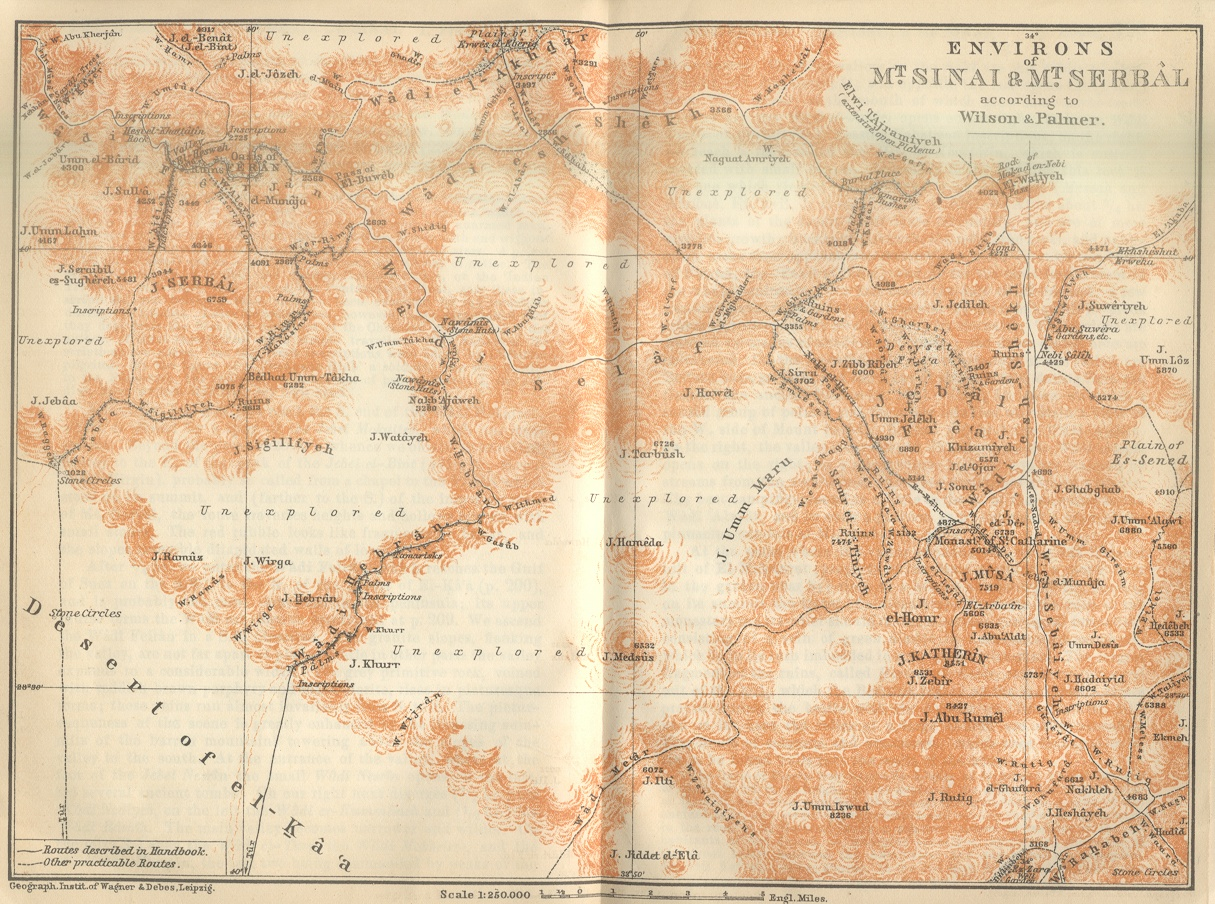
\includegraphics[clip,trim=5cm 2cm 9cm 1cm,width=\linewidth]{OldBookArt--MapImages-173.jpg}
\vfill
{\large \textit{This material is Open Game Content, and is licensed for public use under the terms of the Open Game License v1.0a.}\\
\today}
\end{center}

\pagebreak
\sffamily
\pagestyle{plain}
\raggedbottom

%%%%%%%%%%%%%%%%%%%%%%%%%%%%%%%%%%%%%%%%%%%%%%%%%%
%%%%%%%%%%%%%%%%%%%%%%%%%%%%%%%%%%%%%%%%%%%%%%%%%%
%%% Table of Contents
%%%%%%%%%%%%%%%%%%%%%%%%%%%%%%%%%%%%%%%%%%%%%%%%%%
%%%%%%%%%%%%%%%%%%%%%%%%%%%%%%%%%%%%%%%%%%%%%%%%%%
\renewcommand{\contentsname}{Table of Contents}
\setcounter{tocdepth}{1}
\tableofcontents

%%%%%%%%%%%%%%%%%%%%%%%%%%%%%%%%%%%%%%%%%%%%%%%%%%
%%%%%%%%%%%%%%%%%%%%%%%%%%%%%%%%%%%%%%%%%%%%%%%%%%
%%% Main Content
%%%%%%%%%%%%%%%%%%%%%%%%%%%%%%%%%%%%%%%%%%%%%%%%%%
%%%%%%%%%%%%%%%%%%%%%%%%%%%%%%%%%%%%%%%%%%%%%%%%%%

%% Primary Chapters Here

\clearpage

\chapter{Introduction}
\section{What is a Role-playing Game?}
foo
\section{What You Need To Play}
foo
\section{The Core Mechanic}
foo
\section{Creating a Character}
foo

\chapter{Races}
%need a race basics section here
\raceentry{Aasimar}{``My ancestors were more beautiful than you can imagine."}\\
\begin{multicols}{2}
Aasimar are humans that have a beautiful outsider, usually but not always a celestial, somewhere in their ancestry. \linebreak
\indent\textbf{Personality: }Though mostly human, an aasimar's immortal heritage influences their mental development. Aasimar tend toward more extreme personalities, being especially quiet and introspective or particularly loud and boisterous. Most aasimar are very opinionated, and have strongly held beleifs.\linebreak
\indent\textbf{Physical Description: }Aasimar look like especially beautiful humans, though they sometimes bear vestiges of their ancestry that denote them as being different (strangely colored eyes, silver-blonder or white hair, slightly `off' facial features).\linebreak
\indent\textbf{Society: }Aasimar are typically born and raised in human societies, and gain the same customs of that culture.\linebreak
\indent\textbf{Alignment: }Most aasimar are the descendants of celestials, and tend towards the good alignments. Rarely, an aasimar might instead have an infernal heritage, being the descendant of an erinyes or succubus. Such aasimar instead tend towards an evil alignment.\linebreak

\columnbreak

\racetable
\type{Outsider (Native and Human Subtype)}
\size{Medium}
\speed{30 foot}
\standardsenses
\scores{+2 Wisdom, +2 Charisma}
\racespecial{
\fakeitem{\spell{Light} \sla : An Aasimar with a Charisma of at least 10 may cast \spell{light} as a spell-like ability with a caster level equal to their character level once per day.} \linebreak
\fakeitem{+2 bonus to Spot, and Listen checks.}
}
\autolanguages{Common}
\bonuslanguages{Abyssal, Aquan, Auran, Celestial, Formian, Ignan, Slaad, Sylvan, Terran.}
\favoredclasses{Paladin and Sorcerer}
\end{tabu}

\vspace{\baselineskip}
\agetable{20}{+1d6}{+2d6}{+3d6}

\vspace{\baselineskip}
\male{4' 7"}{+2d8}{90 lb.}{x(2d4)}
\female{4' 5"}{+2d8}{80 lb.}{x(2d4)}
\heightweighttable
\end{multicols}
\begin{racebox}
\raceentry{Drow}{``Time to die for the Spider Queen."}
\begin{multicols}{2}

\begin{racetable}
\type{Humanoid (Elf Subtype)}
\size{Medium}
\scores{+2 Dexterity, -2 Constitution}
\speed{30}
\senses{Darkvision 120'}
\autolanguages{Elvish}
\bonuslanguages{Abyssal, Beholder, Common, Draconic, Drow Sign Language, Dwarvish, Gnome, Kuo-Toa, Terran, Undercommon}
\favoredclasses{Cleric and Wizard}
\end{racetable}

\vspace{\baselineskip}
\agetable{20}{+1d6}{+2d6}{+3d6}

\vspace{\baselineskip}
\begin{heightweighttable}
\male{4' 7"}{+2d8}{90 lb.}{x(2d4)}
\female{4' 5"}{+2d8}{80 lb.}{x(2d4)}
\end{heightweighttable}

\racialtraits{
\racetrait{Daylight Sensitivity}{While in brightly lit surroundings (such as a daylight spell), a Drow suffers a -2 penalty to attack rolls and precision-based skill checks.}
\racetrait{Innate Magic}{Drow with a Charisma of at least 10 may cast deeper darkness (duration 4 hours), and fairie fire as spell-like abilities with a caster level equal to their character level once per day each.}
\racetrait{Magic Resistant}{+2 bonus to saving throws against spells and spell-like abilities.}
\racetrait{Skill Bonus}{+2 bonus to Spot and Listen checks.}
\racetrait{Elven Trance}{Drow never sleep and are immune to sleep effects. Drow must still perform their 4 hour daily trance to stay coherent and rested.}
\racetrait{Interesting Times}{Drow live an exceedingly interesting life and every Drow has proficiency with the rapier and an exotic ranged weapon of their choice.}
}

\end{multicols}
\end{racebox}
\raceentry{Dwarf}
\quot{``I remember that...''}

\listone
		\item Medium Size
		\item 20' movement
		\item Humanoid Type (Dwarf Subtype)
		\item +2 Constitution, -2 Charisma
		\item Dwarves can move up to their full speed even when wearing medium or heavy armor or when carrying a medium or heavy load
		\item Darkvision: Dwarves can see up to 60 feet in the dark.
		\item Stonecunning: This ability grants a dwarf a +2 racial bonus on Search checks to notice unusual stonework, such as sliding walls, stonework traps, new construction (even when built to match the old), unsafe stone surfaces, shaky stone ceilings, and the like. Something that isn’t stone but that is disguised as stone also counts as unusual stonework. A dwarf who merely comes within 10 feet of unusual stonework can make a Search check as if he were actively searching, and a dwarf can use the Search skill to find stonework traps as a rogue can. A dwarf can also intuit depth, sensing his approximate depth underground as naturally as a human can sense which way is up.
		\item Weapon Familiarity: Dwarves may treat dwarven waraxes and dwarven urgroshes as martial weapons, rather than exotic weapons.
		\item Stability: A dwarf gains a +4 bonus on ability checks made to resist being bull rushed or tripped when standing on the ground (but not when climbing, flying, riding, or otherwise not standing firmly on the ground).
		\item +2 racial bonus on saving throws against poison.
		\item +2 racial bonus on saving throws against spells and spell-like effects.
		\item +1 racial bonus on attack rolls against orcs and goblinoids.
		\item +4 dodge bonus to Armor Class against monsters of the giant type. Any time a creature loses its Dexterity bonus (if any) to Armor Class, such as when it’s caught flat-footed, it loses its dodge bonus, too.
		\item +2 racial bonus on Appraise checks that are related to stone or metal items.
		\item +2 racial bonus on Craft checks that are related to stone or metal.
		\item Favored class: Fighter
		\item Automatic Languages: Common and Dwarven.
		\item Bonus Languages: Giant, Gnome, Goblin, Orc, Terran, and Undercommon.
\end{list}

\raceentry{Elf}
\quot{``You shall never harm my beautiful trees!''}

\listone
		\item Medium Size
		\item Humanoid Type (Elf Subtype)
		\item 30' movement
		\item +2 Dexterity, -2 Constitution
		\item Low Light Vision: Elves can see twice as far as a human in poor lighting.
		\item Weapon Proficiency: Elves are proficient with the longsword, rapier, longbow (including composite longbow), and shortbow (including composite shortbow).
		\item +2 racial bonus on Listen, Search, and Spot checks. An elf who merely passes within 5 feet of a secret or concealed door is entitled to a Search check to notice it as if she were actively looking for it.
		\item Favored Class: Wizard.
		\item Automatic Languages: Common and Elven. 
		\item Bonus Languages: Draconic, Gnoll, Gnome, Goblin, Orc, and Sylvan.
\end{list}
\raceentry{Feytouched}
\quot{``All my life, I have never fit in. Not in town, not in the forest. In some integral fashion I am unlike those around me, and I believe it is my fate to live and die alone."}

\listone
		\item Medium Size
    \item Fey Type
    \item 30' movement
    \item Low-Light Vision: Feytouched can twice as far as a human in poor lighting.
    \item +2 Dexterity, +2 Charisma, -2 Constitution. Feytouched are graceful and those which are not beautiful are terrifying, but they are fragile like flowers.
    \item Immunity to [Compulsion] Effects
    \item Magic Affinity: Every Feytouched is different, and marked by the signature magics of the fey in a different manner. Every Feytouched has one spell that can be used once per day as a spell-like ability. This spell is chosen at 1st level and cannot be changed. Any 1st level Illusion or Enchantment spell from the Sorcerer/Wizard list is fair game, and the save DC is Charisma-based.
    \item Favored Class: Bard
    \item Feytouched speak Common and Sylvan. Bonus Languages may be selected from the following list:
      Aquan, Auran, Elvish, Draconic, Dwarvish, Druidic, Goblin, Gnoll, Gnome, Halfling.
\end{list}
\begin{racebox}
\raceentry{Gnome}{``What's that you say little mole? Kobolds in the well!?"}
\begin{multicols}{2}

\begin{racetable}
\type{Humanoid (Gnome subtype)}
\size{Small}
\scores{+2 Constitution, --2 Strength}
\speed{20}
\senses{Low Light Vision}
\autolanguages{Common and Gnome}
\bonuslanguages{Draconic, Dwarven, Elven, Giant, Goblin, and Orc. In addition, a gnome can speak with a burrowing mammal (a badger, fox, rabbit, or the like).}
\favoredclasses{Bard}
\end{racetable}

Nothing until we find or write it.

\racedescription{NYW}

\racepersonality{NYW}

\racesociety{NYW}

\racealignment{NYW}

\racialtraits{
\racetrait{Weapon Familiarity}{Gnomes may treat gnome hooked hammers as martial weapons rather than exotic weapons.}
\racetrait{+2 racial bonus on saving throws against illusions.}
\racetrait{Add +1 to the Difficulty Class for all saving throws against illusion spells cast by gnomes. This adjustment stacks with those from similar effects.}
\racetrait{+1 racial bonus on attack rolls against kobolds and goblinoids.}
\racetrait{+4 dodge bonus to Armor Class against monsters of the giant type.}
\racetrait{+2 racial bonus on Listen checks.}
\racetrait{+2 racial bonus on Craft (alchemy) checks.}
\racetrait{Spell-Like Abilities: 1/day—speak with animals (burrowing mammal only, duration 1 minute). A gnome with a Charisma score of at least 10 also has the following spell-like abilities: 1/day—dancing lights, ghost sound, prestidigitation. Caster level 1st; save DC 10 + gnome’s Cha modifier + spell level.} % I'm pretty sure there's a much better way to format this, say by using the \sla used for aasimar. That Cha req goofs it up.
}


%\columnbreak

\vspace{\baselineskip}
\agetable{40}{+4d6}{+6d6}{+9d6}

\vspace{\baselineskip}
\begin{heightweighttable}
\male{3' 0"}{+2d4}{40 lb.}{x(1)}
\female{2' 10"}{+2d4}{35 lb.}{x(1)}
\end{heightweighttable}
\end{multicols}
\end{racebox}
\raceentry{Goblin}
\quot{``You weren't hired to think. You were hired because you have opposable thumbs."}

\listone
    \item Small Size
    \item 30' movement (despite small size).
    \item Humanoid Type (Goblinoid subtype)
    \item Darkvision: Goblins can see up to 60 feet in the dark.
    \item +2 Dexterity, -2 Strength, -2 Charisma
    \item +4 bonus to Move Silently and Ride checks.
    \item Bonus Feat: Mounted Combat
    \item Goblins benefit from an ancient pact with the Worgs, and every Goblin receives a +2 bonus to any Bluff, Diplomacy, Handle Animal, Sense Motive, or Survival check made with respect to a Worg.
    \item Favored Classes: Rogue and Wizard
    \item Automatic Languages: Common, Goblin
    \item Bonus Languages: Draconic, Elvish, Dwarvish, Giant, Gnoll, Infernal, Orcish, Undercommon, and Worg.
\end{list}
\raceentry{Half-Elf}
\quot{``I don't fit in anywhere, please, listen to me cry.''}

\listone
		\item Medium Size
		\item 30' Movement
		\item Humanoid Type
		\item Low-Light Vision: Half-Elves can see twice as humans in poor lighting.
		\item Immunity to sleep spells and similar magical effects, and a +2 racial bonus on saving throws against enchantment spells or effects.
		\item +1 racial bonus on Listen, Search, and Spot checks.
		\item +2 racial bonus on Diplomacy and Gather Information checks.
		\item Elven Blood: For all effects related to race, a half-elf is considered an elf.
		\item Favored Class: Any
		\item Automatic Languages: Common and Elven.
		\item Bonus Languages: Any (other than secret languages, such as Druidic).
\end{list}
\raceentry{Half-Orc}
\quot{``I don't fit in anywhere, but you may be surprised to know that this dagger fits all kinds of places."}

\listone
    \item Medium Size
    \item 30' movement
    \item Humanoid Type (Orc and Human subtype)
    \item Darkvision: Half-Orcs can see up to 60 feet in the dark.
    \item +2 Strength
    \item +2 to Intimidate, Gather Information, and Survival checks.
    \item Favored Classes: Assassin and Barbarian
    \item Automatic Languages: Orc, Common
    \item Bonus Languages: Any.
\end{list}
\subsection{Halfling}
\quot{``Where are we going Mr. Frodo?''}

\listone
		\item Small Size
		\item 20' movement
		\item +2 Dexterity, -2 Strength
		\item +2 racial bonus on Climb, Jump, Listen, and Move Silently checks.
		\item +1 racial bonus on all saving throws.
		\item +2 morale bonus on saving throws against fear: This bonus stacks with the halfling’s +1 bonus on saving throws in general.
		\item +1 racial bonus on attack rolls with thrown weapons and slings.
		\item Favored Class: Rogue
		\item Automatic Languages: Common and Halfling.
		\item Bonus Languages: Dwarven, Elven, Gnome, Goblin, and Orc.
\end{list}		

\raceentry{Hobgoblin}
\quot{``That's some tough talk from a man who wears a basket on his head."}

\listone
    \item Medium Size
    \item 30' movement.
    \item Humanoid Type (Goblinoid subtype)
    \item Darkvision: Hobgoblins can see up to 60 feet in the dark.
    \item +2 Dexterity, +2 Constitution
    \item +4 bonus to Move Silently checks.
    \item Favored Classes: Fighter and Samurai
    \item Automatic Languages: Common, Goblin
    \item Bonus Languages: Draconic, Elvish, Dwarvish, Giant, Gnoll, Ignan, Infernal, Orcish.
\end{list}
\raceentry{Human}
\quot{``Yeah, I'm pretty normal.''}

\listone
	\item Medium Size
	\item 30' movement.
	\item Humanoid Type (Human subtype)
	\item 1 extra feat at 1st level.
	\item 4 extra skill points at 1st level and 1 extra skill point at each additional level.
	\item Favored Class: Any. When determining whether a multiclass human takes an experience point penalty, his or her highest-level class does not count.
	\item Automatic Language: Common. 
	\item Bonus Languages: Any (other than secret languages, such as Druidic). See the Speak Language skill.
\end{list}
\raceentry{Kobold}
\quot{``Aieeeeeeeee!''}

\listone
		\item Small Size
		\item 30' movement (despite small size)
		\item Humanoid Type (Reptilian subtype)
		\item Darkvision: Kobolds can see up to 60 feet in the dark.
		\item -4 Strength, +2 Dexterity, -2 Constitution
		\item Racial Skills: A kobold character has a +2 racial bonus on Craft (trapmaking), Profession (miner), and Search checks.
		\item +1 natural armor bonus.
		\item Light sensitivity: Kobolds are dazzled in bright sunlight or within the radius of a daylight spell. 
		\item Favored Class: Sorcerer.
		\item Automatic Languages: Draconic.
		\item Bonus Languages: Common, Undercommon.
\end{list}
\raceentry{Orc}
\quot{``Waaarrrggghhhh!"}

\listone
    \item Medium Size
    \item 30' movement.
    \item Humanoid Type (Orc subtype)
    \item Darkvision: Orcs can see up to 60 feet in the dark.
    \item +4 Strength, -2 Intelligence, -2 Charisma, -2 Wisdom
    \item Daylight Sensitivity: While in brightly lit surroundings (such as a daylight spell), an Orc suffers the dazzled condition and is thus at a -1 penalty to attack rolls and precision-based skill checks.
    \item +2 bonus to saving throws vs. Poison and Disease.
    \item Immunity to ingested poisons.
    \item +2 to Jump and Survival checks.
    \item Favored Classes: Barbarian and Cleric
    \item Automatic Languages: Orc, Common
    \item Bonus Languages: Dwarvish, Elvish, Giant, Gnoll, Goblin, Sylvan, Undercommon.
\end{list}
\raceentry{Tiefling}
\quot{``My ancestors were more evil than you will ever know, but let's see how I compare.''}

\listone
    \item Medium Size
    \item 30' movement.
    \item Outsider Type (Native and Human subtype)
    \item Darkvision: Tieflings can see up to 60 feet in the dark.
    \item +2 Dexterity, +2 Intelligence, -2 Charisma
    \item Tieflings with a Charisma of at least 10 may cast darkness as a spell-like ability with a caster level equal to their character level once per day.
    \item +2 bonus to Bluff, Hide, and Move Silently checks.
    \item Favored Classes: Rogue and True Fiend
    \item Automatic Languages: Common
    \item Bonus Languages: Abyssal, Aquan, Auran, Celestial, Formian, Ignan, Slaad, Sylvan, Terran.
\end{list}

\chapter{Classes}
\section{Class Basics}
foo

\classname{Assassin} \label{class:assassin}
\vspace{-8pt}
\quot{"I kill people. Individually, you are a person. Collectively, I think you count as people."}

\desc{An assassin is a master of the art of killing, a vicious weapon honed by experience and inclination to learn the myriad ways to end a life. Unlike common warriors or rogues, an Assassin does not study various fighting arts or muddle his training with martial dirty tricks, he instead studies the anatomy of the various creatures of wildly different anatomies and forms of existence, and he uses this knowledge to place his blows in areas vital for biological or mystical reasons. Stealth and sudden violence are his hallmarks, and various exotic tools and killing methods become his tools.}

\desc{While most societies consider assassination to be a vile art, or at best a dishonorable or unvalorous one, the reasons that drive these killers vary. Cold-hearted mercenaries share a skill set with dedicated demon-hunters, differing only in the application of their skills. Only the most na\"ive student of ethics believes that all killing is evil, or that nobility cannot be found in a mercifully quick death.}

\ability{Alignment:}{An Assassin may be of any alignment.}

\ability{Races:}{Any}

\ability{Starting Gold:}{6d4x10 gp (150 gold)}

\ability{Starting Age:}{As Rogue.}

\ability{Hit Die:}{d6}

\ability{Class Skills:}{The Assassin's skills (and the key ability for each skill) are Balance (Dex), Bluff (Cha), Climb (Str), Concentration (Con), Craft (Int), Diplomacy (Cha), Disable Device (Int), Disguise (Cha), Gather Information (Cha), Hide (Dex), Intimidate (Cha), Jump (Str), Knowledge (all) (Int), Listen (Wis), Move Silently (Dex), Perform (Cha), Profession (Wis), Search (Int), Sense Motive (Wis), Sleight of Hand (Dex), Spellcraft (Int), Spot (Wis), Swim (Str), Tumble (Dex), and Use Magic Device (Cha).}

\ability{Skills/Level:}{6 + Intelligence Bonus}

\begin{table}[htb]
\begin{small}
\begin{tabular}{lp{1.9cm}p{0.7cm}p{0.7cm}p{0.7cm}l}
Level  &Base Attack Bonus &Fort Save &Ref Save &Will Save &Special\\
1st &+0 &+2 &+2 &+0 &Poison Use, Death Attack +3d6, Personal Immunity, Spellcasting\\
2nd &+1 &+3 &+3 &+0 &Uncanny Dodge, Death Attack +4d6\\
3rd &+2 &+3 &+3 &+1 &Hide in Plain Sight, Death Attack +5d6\\
4th &+3 &+4 &+4 &+1 &Cloak of Discretion, Death Attack +6d6\\
5th &+3 &+4 &+4 &+1 &Traps, Trapmaking, Death Attack +7d6\\
6th &+4 &+5 &+5 &+2 &Palm Weapon, Death Attack +8d6\\
7th &+5 &+5 &+5 &+2 &Full Death Attack, Death Attack +9d6\\
8th &+6/+1 &+6 &+6 &+2 &Nerve of the Assassin, Death Attack +10d6\\
9th &+6/+1 &+6 &+6 &+3 &Improved Uncanny Dodge, Death Attack +11d6\\
10th &+7/+2 &+7 &+7 &+3 &Skill Mastery, Death Attack +12d6\\
11th &+8/+3 &+7 &+7 &+3 &Poisonmaster, Death Attack +13d6\\
12th &+8/+3 &+8 &+8 &+4 &Personal Immunity, Death Attack +14d6\\
13th &+9/+4 &+8 &+8 &+4 &Exotic Method, Death Attack +15d6\\
14th &+10/+5 &+9 &+9 &+4 &Personal Immunity, Death Attack +16d6\\
15th &+11/+6/+6 &+9 &+9 &+5 &Killer's Proof, Death Attack +17d6\\
16th &+12/+7/+7 &+10 &+10 &+5 &Exotic Method, Death Attack +18d6\\
17th &+12/+7/+7 &+10 &+10 &+5 &Death by a Thousand Cuts, Death Attack +19d6\\
18th &+13/+8/+8 &+11 &+11 &+6 &Mind Blank, Death Attack +20d6\\
19th &+14/+9/+9 &+11 &+11 &+6 &Exotic Method, Death Attack +21d6\\
20th &+15/+10/+10 &+12 &+12 &+6 &Killing Strike, Death Attack +22d6\\
\end{tabular}
\end{small}
\end{table}

\begin{floatingfigure}{3.9in}
\begin{small}
\noindent\begin{tabular}{lllllllllllllllll}
 & \multicolumn{7}{c}{Assassin Spells Per Day}  &   &\multicolumn{7}{c}{Assassin Spells Known}\\
  &0 &1 &2 &3 &4 &5 &6 &  &  &0 &1 &2 &3 &4 &5 &6\\
1 &2 &- &- &- &- &- &- &  &1 &4 &- &- &- &- &- &-\\
2 &3 &0 &- &- &- &- &- &  &2 &5 &2 &- &- &- &- &-\\
3 &3 &1 &- &- &- &- &- &  &3 &6 &3 &- &- &- &- &-\\
4 &3 &2 &0 &- &- &- &- &  &4 &6 &3 &2 &- &- &- &-\\
5 &3 &3 &1 &- &- &- &- &  &5 &6 &4 &3 &- &- &- &-\\
6 &3 &3 &2 &- &- &- &- &  &6 &6 &4 &3 &- &- &- &-\\
7 &3 &3 &2 &0 &- &- &- &  &7 &6 &4 &4 &2 &- &- &-\\
8 &3 &3 &3 &1 &- &- &- &  &8 &6 &4 &4 &3 &- &- &-\\
9 &3 &3 &3 &2 &- &- &- &  &9 &6 &4 &4 &3 &- &- &-\\
10 &3 &3 &3 &2 &0 &- &- &  &10 &6 &4 &4 &4 &2 &- &-\\
11 &3 &3 &3 &3 &1 &- &- &  &11 &6 &4 &4 &4 &3 &- &-\\
12 &3 &3 &3 &3 &2 &- &- &  &12 &6 &4 &4 &4 &3 &- &-\\
13 &3 &3 &3 &3 &2 &0 &- &  &13 &6 &4 &4 &4 &4 &2 &-\\
14 &3 &3 &3 &3 &3 &1 &- &  &14 &6 &4 &4 &4 &4 &3 &-\\
15 &3 &3 &3 &3 &3 &2 &- &  &15 &6 &4 &4 &4 &4 &3 &-\\
16 &3 &3 &3 &3 &3 &2 &0 &  &16 &6 &5 &4 &4 &4 &4 &2\\
17 &3 &3 &3 &3 &3 &3 &1 &  &17 &6 &5 &5 &4 &4 &4 &3\\
18 &3 &3 &3 &3 &3 &3 &2 &  &18 &6 &5 &5 &5 &4 &4 &3\\
19 &3 &3 &3 &3 &3 &3 &3 &  &19 &6 &5 &5 &5 &5 &4 &4\\
20 &3 &3 &3 &3 &3 &3 &3 &  &20 &6 &5 &5 &5 &5 &5 &4\\
\end{tabular}
\end{small}
\end{floatingfigure}

\smallskip\noindent All of the following are Class Features of the Assassin class.

\ability{Weapon and Armor Proficiency:}{Assassins are proficient with all Light Weapons, as well as simple weapons, repeating crossbows, and hand crossbows. At first level, an Assassin gains proficiency with one Exotic Weapon of her choice. Assassins are proficient with Light Armor but not with shields.}

\ability{Spellcasting:}{The Assassin is an Arcane Spellcaster with the same spells per day and spells known progression as a Bard, except that he gains no more than three spell slots per level. An Assassin's spells known may be chosen from the Sorcerer/Wizard list, and must be from the schools of Divination, Illusion, or Necromancy. To cast an Assassin spell, she must have an Intelligence at least equal to 10 + the Spell level. The DC of the Assassin's spells is Intelligence based and the bonus spells are Intelligence based.}

\ability{Poison Use (Ex):}{An Assassin may prepare, apply, and use poison without any chance of poisoning herself.}

\ability{Death Attack (Ex):}{An Assassin may spend a full-round action to study an opponent who would be denied their Dexterity bonus if she instead attacked that target. If she does so, her next attack is a Death Attack if she makes it within 1 round. A Death Attack inflicts a number of extra dice of damage equal to her Assassin level plus two dice, but only if the target is denied its Dexterity Bonus to AC against that attack. Special attacks such as a coup de grace may be a Death Attack. Assassins are well trained in eliminating magical or distant opponents, and do not have to meet the stringent requirements of a sneak attack, though if a character has both sneak attack and death attack, they stack if the character meets the requirements of both. As long as the victim is denied their dexterity against attacks from the assassin during the study action and the attack itself, it counts as a death attack. An Assassin may load a crossbow simultaneously with his action to study his target if he has a Base Attack Bonus of +1 or more.}

\ability{Personal Immunity (Ex):}{Choose four poisons, an Assassin is immune to all four of those poisons, even if they are made available in a stronger strength. At levels 5, 7, and 12 the Assassin may choose one more type of poison to become immune to. At level 14, an Assassin becomes immune to all poisons.}

\ability{Uncanny Dodge (Ex):}{Starting at 2nd level, an Assassin can react to danger before his senses would normally allow him to do so. He retains her Dexterity bonus to AC (if any) even if she is caught flat-footed or struck by an invisible attacker. However, he still loses her Dexterity bonus to AC if immobilized. If an Assassin already has uncanny dodge from a different class he automatically gains improved uncanny dodge (see below) instead.}

\ability{Hide in Plain Sight (Ex):}{A 3rd level Assassin can hide in unusual locations, and may hide in areas without cover or concealment without penalty. An Assassin may even hide while being observed. This ability does not remove the -10 penalty for moving at full speed, or the -20 penalty for running or fighting.}

\ability{Cloak of Discretion (Su):}{At 4th level, an Assassin is protected by a constant \emph{nondetection} effect, with a caster level equal to his character level.}

\ability{Trapfinding:}{At 5th level, Assassins can use the Search skill to locate traps when the task has a Difficulty Class higher than 20. Finding a nonmagical trap has a DC of at least 20, or higher if it is well hidden. Finding a magic trap has a DC of 25 + the level of the spell used to create it. Assassins can use the Disable Device skill to disarm magic traps. A magic trap generally has a DC of 25 + the level of the spell used to create it. An Assassin who beats a trap's DC by 10 or more with a Disable Device check can study a trap, figure out how it works, and bypass it (with her party) without disarming it.}

\ability{Trapmaking:}{At 5th level, the Assassin learns to build simple mechanical traps in out of common materials. As long as has access to ropes, flexible material like green wood, and weapon-grade materials like sharpened wooden sticks or steel weapons, he can build an improvised trap in 10 minutes. He can build any non-magical trap on the "CR 1" trap list that doesn't involve a pit. These traps have a Search DC equal to 20 + the Assassin's level, have a BAB equal to his own, and are always single-use traps. He may add poison to these traps, if he has access to it, but it will dry out in an hour.}

\ability{Palm Weapon (Su):}{At 6th level, the Assassin learns to conceal weapons with supernatural skill. Any weapon successfully concealed with Sleight of Hand cannot be found with divination magic.}

\ability{Full Death Attack:}{At 7th level, if the Assassin studies an opponent to perform a Death Attack, she can make a full attack during the next round where every attack inflicts Death Attack damage as long as the target was denied their Dexterity bonus to AC against the first attack in the full attack action.}

\ability{Nerve of the Killer:}{At 8th level, an Assassin gains a limited immunity to compulsion and charm effects. While studying a target for a Death Attack, and for one round afterward, he counts as if he were within a \spell{protection from evil} effect. This does not confer a deflection bonus to AC.}

\ability{Improved Uncanny Dodge (Ex):}{An Assassin of 9th level or higher can no longer be flanked. This defense denies another character the ability to sneak attack the character by flanking him, unless the attacker has at least four more levels in a class that provides sneak attack than the target. If a character already has uncanny dodge (see above) from a second class, the character automatically gains improved uncanny dodge instead, and the levels from the classes that grant uncanny dodge stack to determine the minimum level required to flank the character.}

\ability{Skill Mastery (Ex):}{At 10th level, an Assassin becomes so certain in the use of certain skills that she can use them reliably even under adverse conditions. When making a skill check with Climb, Disable Device, Hide, Move Silently, Search, Spellcraft, Use Magic Device, Use Rope, or Swim, she may take 10 even if stress and distractions would normally prevent her from doing so.}

\ability{Poisonmaster:}{At 11th level, the Assassin learns alchemic secrets for creating short-term poisons. By expending an entire healer's kit worth of materials and an hour of time, he can synthesize one dose of any poison in the DMG. This poison degrades to uselessness in one week.}

\ability{Exotic Method:}{At 13th, 16th, and 19th level the Assassin learns an exotic form of killing from the list below. Once chosen, this ability does not change:}
\listone

    \item \ability{Carrier:}{Three times per day, the Assassin can cast \spell{contagion} as a swift action spell-like ability.}
    \item \ability{Poison of the Cockatrice:}{Twice per day, the Assassin can cast \spell{flesh to stone} as a swift action spell-like ability.}
    \item \ability{Killer Faerie Arts:}{Twice per day, the Assassin can cast \spell{polymorph other} as a swift action spell-like ability.}
    \item \ability{Proxy Assassin:}{Twice per day, the Assassin can cast \spell{summon monster VII} as a spell-like ability. This effect lasts 10 minutes.}
    \item \ability{Death By Plane:}{Once per day, the Assassin can cast \spell{plane shift} as a spell-like ability.}
    \item \ability{Dimesional Rip:}{Once per day, the Assassin can cast \spell{implosion} as a spell-like ability. The duration of this effect is three rounds.}
    \item \ability{New School:}{The Assassin may now choose spells known from a new school.}
\end{list}
\vspace{8pt}

\ability{Killer's Proof (Su):}{At 15th level, the Assassin learns to steal the souls of those he kills. If he is holding an onyx worth at least 100 GP when he kills an enemy, he may place their soul within the gem as if he has cast \spell{soul bind} on them at the moment of their death.}

\ability{Death by a Thousand Cuts:}{At 17th level, the assassin has learned to kill even the hardiest of foes by reducing their physical form to shambles. Every successful Death attack inflicts a cumulative -2 Dexterity penalty to the Assassin's victim. These penalties last one day.}

\ability{Mind Blank (Su):}{At 18th level, the Assassin is protected by a constant \spell{mind blank} effect.}

\ability{Killing Strike (Su):}{At 20th level, the Assassin's Death Attacks bypass his victim's DR and hardness.}


\classname{Barbarian} \label{class:barbarian}
\vspace{-8pt}
\quot{''My name is Sharptooth of the Wolf Tribe. Your women, lands, and riches are mine.''}

\ability{Playing a Barbarian:}{Playing a Barbarian is actually very easy. In general, you hit things, and they fall down. A Barbarian's action in almost any circumstance can plausibly be ''I hit it with my great axe!" As such, a Barbarian character can be a good method to introduce a new player to the game or kill some orcs when you've had a few glasses of brew.}

\ability{Alignment:}{Every alignment has its share of Barbarians, however more Barbarians are of Chaotic alignment than of Lawful Alignment.}

\ability{Races:}{Anybody can become a barbarian, and in areas with little in the way of civilization, a lot of people do.}

\ability{Starting Gold:}{4d6x10 gp (140 gold)}

\ability{Starting Age:}{As Barbarian.}

\ability{Hit Die:}{d12}

\ability{Class Skills:}{The Barbarian's class skills (and the key ability for each skill) are Balance (Dex), Climb (Str), Hide (Dex), Intimidate (Cha), Jump (Str), Knowledge: Nature (Int), Listen (Wis), Move Silently (Dex), Sense Motive (Wis), Spot (Wis), Survival (Wis), and Swim (Str).}

\ability{Skills/Level:}{4 + Intelligence Bonus}

\begin{table}[htb]
\begin{small}
\begin{tabular}{lp{3cm}p{0.7cm}p{0.7cm}p{0.7cm}l}
Level  &Base Attack Bonus &Fort Save &Ref Save &Will Save &Special\\
1st &+1 &+2 &+0 &+0 &Rage, Fast Healing 1\\
2nd &+2 &+3 &+0 &+0 &Rage Dice +1d6, Combat Movement +5'\\
3rd &+3 &+3 &+1 &+1 &Battle Hardened\\
4th &+4 &+4 &+1 &+1 &Rage Dice +2d6, Combat Movement +10'\\
5th &+5 &+4 &+1 &+1 &Sidestep Hazards , Fast Healing 5\\
6th &+6/+1 &+5 &+2 &+2 &Rage Dice +3d6, Combat Movement +15'\\
7th &+7/+2 &+5 &+2 &+2 &Great Blows\\
8th &+8/+3 &+6 &+2 &+2 &Rage Dice +4d6, Combat Movement +20'\\
9th &+9/+4 &+6 &+3 &+3 &Great Life\\
10th &+10/+5 &+7 &+3 &+3 &Rage Dice +5d6, Combat Movement +25', Fast Healing 10\\
11th &+11/+6/+6 &+7 &+3 &+3 &Call the Horde\\
12th &+12/+7/+7 &+8 &+4 &+4 &Rage Dice +6d6, Combat Movement +30'\\
13th &+13/+8/+8 &+8 &+4 &+4 &Watched by Totems\\
14th &+14/+9/+9 &+9 &+4 &+4 &Rage Dice +7d6, Combat Movement +35'\\
15th &+15/+10/+10 &+9 &+5 &+5 &Primal Assault, Fast Healing 15\\
16th &+16/+11/+11/+11 &+10 &+5 &+5 &Rage Dice +8d6, Combat Movement +40'\\
17th &+17/+12/+12/+12 &+10 &+5 &+5 &Savagery\\
18th &+18/+13/+13/+13 &+11 &+6 &+6 &Rage Dice +9d6, Combat Movement +45'\\
19th &+19/+14/+14/+14 &+11 &+6 &+6 &One With The Beast\\
20th &+20/+15/+15/+15 &+12 &+6 &+6 &Rage Dice +10d6, Combat Movement +50', Fast Healing 20\\
\end{tabular}
\end{small}
\end{table}

\smallskip\noindent All of the following are Class Features of the Barbarian class.


\ability{Weapon and Armor Proficiency:}{Barbarians are proficient with simple weapons, martial weapons, light armor, medium armor and with shields.}

\ability{Rage (Ex):}{When doing melee damage to a foe or being struck by a foe, a Barbarian may choose to enter a Rage as an immediate action. While Raging, a Barbarian gains a +2 morale bonus to hit and damage in melee combat and may apply any Rage Dice he has to his melee damage rolls. He also gains a +2 to saves, a -2 to AC, and he gains DR X/-- with ''X" being equal to half his Barbarian level +2 (rounded down). For example, a 1st level Barbarian has DR 3/-- while Raging and a 10th level Barbarian has DR 7/-- while Raging. While Raging, a Barbarian may not cast spells, activate magic items, use spell-like abilities, or drop his weapons or shield. Rage lasts until he has neither struck an enemy for three consecutive rounds nor suffered damage from an enemy for three consecutive rounds. He may voluntarily end a Rage as a full-round action.}

\ability{Fast Healing:}{Barbarians shrug off wounds that would cripple a lesser man, and have learned to draw upon deep reserves of energy and stamina. At 1st level, they gain Fast Healing 1. At 5th level this becomes Fast Healing 5, Fast Healing 10 at 10th level, Fast Healing 15 at 15th level, and Fast Healing 20 at 20th level. This healing only applies while he is not raging. \smallskip

If a Barbarian ever multiclasses, he permanently loses this ability. A multiclass character does not gain this ability.  A character with 4 or more levels of Barbarian gains this ability even if multiclassed.}

\ability{Rage Dice:}{While Raging, a Barbarian may add these dice of damage to each of his melee attacks. These dice are not multiplied by damage multipliers, and are not applied to any bonus attacks beyond those granted by Base Attack Bonus. These dice are not sneak attack dice, and do not count as sneak attack dice for the prerequisites of prestige classes or feats.}

\ability{Combat Movement:}{While Raging, a Barbarian moves faster in combat, and may add his Combat Movement to his speed when he takes a move action to move.}

\ability{Battle Hardened:}{At 3th level, a Raging Barbarian's mind has been closed off from distractions by the depths of his bloodlust and battle fury. While Raging, he may use his Fortitude Save in place of his Will Save. If he is under the effects of a compulsion or fear effect, he may act normally while Raging as if he was inside a \spell{protection from evil} effect.}

\ability{Sidestep Hazards (Ex):}{At 5th level, a Raging Barbarian learns to sidestep hazards with an intuitive and primal danger sense. While Raging, he may use his Fortitude Save in place of his Reflex Save.}

\ability{Great Blows (Ex):}{At 7th level, a Raging Barbarian's melee attacks are Great Blows. Any enemy struck by the Barbarian's melee or thrown weapon attacks must make a Fort Save or be stunned for one round. No enemy can be targeted by this ability more than once a round, and the save DC for this ability is 10 + half the Barbarian's HD + his Constitution modifier.}

\ability{Great Life (Ex):}{While Raging, a 9th level Barbarian is immune to nonlethal damage, death effects, stunning, critical hits, negative levels, and ability damage (but not ability drain).}

\ability{Call the Horde (Ex):}{An 11th level Barbarian becomes a hero of his people. He gains the Command feat as a bonus feat, but his followers must be Barbarians. In campaigns that do not use Leadership feats, he instead gains a +2 unnamed bonus to all saves.}

\ability{Watched by Totems (Ex):}{At 13th level, a Barbarian may immediately reroll any failed save. He may do this no more than once per failed save.}

\ability{Primal Assault (Ex):}{At 15th level, a Raging Barbarian may choose to radiate an effect similar to an \spell{antimagic field} when he enters a Rage, with a caster level equal to his HD. Unlike a normal antimagic field, this effect does not suppress magic effects on him or the effects of magic items he is wearing or holding.}

\ability{Savagery (Ex):}{At 17th level, a Raging Barbarian may take a full round action to make a normal melee attack that has an additional effect similar to a \spell{mordenkainen's disjunction}. Unlike a normal \spell{mordenkainen's disjunction}, this effect only targets a single item or creature struck.}

\ability{One With The Beast:}{At 19th level, a Barbarian may no longer needs to be in a Rage to use any Barbarian ability.}

%\input{Bard}
\classname{Cleric} \label{class:cleric}
\vspace{-8pt}
\quot{``Fear my righteous shining holy beacon of... righteousness?''}

\desc{Clerics are the holy (or unholy) warriors, standing fast against the darkness (or light). They are also made of cheese, and thus a prime target for minmaxxers.}
% somebody seriously needs to write some better content.
%   - Ak

\ability{Alignment:}{A cleric�s alignment must be within one step of his deity's (that is, it may be one step away on either the lawful-chaotic axis or the good-evil axis, but not both). A cleric may not be neutral unless his deity's alignment is also neutral.}

\ability{Starting Gold:}{5d4x10	gp (125 Gold)}

\ability{Starting Age:}{As Cleric}

\ability{Hit Die:}{d8}

\ability{Class Skills:}{The cleric's class skills (and the key ability for each skill) are Concentration (Con), Craft (Int), Diplomacy (Cha), Heal (Wis), Knowledge (arcana) (Int), Knowledge (history) (Int), Knowledge (religion) (Int), Knowledge (the planes) (Int), Profession (Wis), and Spellcraft (Int).}

\ability{Domains and Class Skills:}{A cleric who chooses the Animal or Plant domain adds Knowledge (nature) (Int) to the cleric class skills listed above. A cleric who chooses the Knowledge domain adds all Knowledge (Int) skills to the list. A cleric who chooses the Travel domain adds Survival (Wis) to the list. A cleric who chooses the Trickery domain adds Bluff (Cha), Disguise (Cha), and Hide (Dex) to the list. See Deity, Domains, and Domain Spells, below, for more information.}

\ability{Skills/Level:}{2 + Intelligence Bonus}

\begin{table}[htb]
\begin{small}
\begin{tabular}{lp{2cm}p{0.7cm}p{0.7cm}p{0.7cm}l llllllllll}
Level  &Base Attack Bonus &Fort Save &Ref Save &Will Save &Special & \multicolumn{10}{c}{Spells Per Day}\\
       &                &    &    &    &                        &0 &1 &2 &3 &4 &5 &6 &7 &8 &9 \\
1st    &+0              &+2  &+0  &+2  & Turn or Rebuke Undead  &3 &1 &- &- &- &- &- &- &- &- \\
2nd    &+1              &+3  &+0  &+3  &                        &4 &2 &- &- &- &- &- &- &- &- \\
3rd    &+2              &+3  &+1  &+3  &                        &4 &2 &1 &- &- &- &- &- &- &- \\
4th    &+3              &+4  &+1  &+4  &                        &5 &3 &2 &- &- &- &- &- &- &- \\
5th    &+3              &+4  &+1  &+4  &                        &5 &3 &2 &1 &- &- &- &- &- &- \\
6th    &+4              &+5  &+2  &+5  &                        &5 &3 &3 &2 &- &- &- &- &- &- \\
7th    &+5              &+5  &+2  &+5  &                        &6 &4 &3 &2 &1 &- &- &- &- &- \\
8th    &+6/+1           &+6  &+2  &+6  &                        &6 &4 &3 &3 &2 &- &- &- &- &- \\
9th    &+6/+1           &+6  &+3  &+6  &                        &6 &4 &4 &3 &2 &1 &- &- &- &- \\
10th   &+7/+2           &+7  &+3  &+7  &                        &6 &4 &4 &3 &3 &2 &- &- &- &- \\
11th   &+8/+3           &+7  &+3  &+7  &                        &6 &5 &4 &4 &3 &2 &1 &- &- &- \\
12th   &+8/+3           &+8  &+4  &+8  &                        &6 &5 &4 &4 &3 &3 &2 &- &- &- \\
13th   &+9/+4           &+8  &+4  &+8  &                        &6 &5 &5 &4 &4 &3 &2 &1 &- &- \\
14th   &+10/+5          &+9  &+4  &+9  &                        &6 &5 &5 &4 &4 &3 &3 &2 &- &- \\
15th   &+11/+6/+6       &+9  &+5  &+9  &                        &6 &5 &5 &5 &4 &4 &3 &2 &1 &- \\
16th   &+12/+7/+7       &+10 &+5  &+10 &                        &6 &5 &5 &5 &4 &4 &3 &3 &2 &- \\
17th   &+12/+7/+7       &+10 &+5  &+10 &                        &6 &5 &5 &5 &5 &4 &4 &3 &2 &1 \\
18th   &+13/+8/+8       &+11 &+6  &+11 &                        &6 &5 &5 &5 &5 &4 &4 &3 &3 &2 \\
19th   &+14/+9/+9       &+11 &+6  &+11 &                        &6 &5 &5 &5 &5 &5 &4 &4 &3 &3 \\
20th   &+15/+10/+10     &+12 &+6  &+12 &                        &6 &5 &5 &5 &5 &5 &4 &4 &4 &4 \\
\end{tabular}
\end{small}
\end{table}

%Theres no way the table would fit with the '+1's in the spells per day section, so I took it out, the text is pretty clear that you get an extra spell slot for your domain.  Feel free to break it into two tables if you think its best.

\smallskip\noindent All of the following are class features of the cleric.

\ability{Weapon and Armor Proficiency:}{Clerics are proficient with all simple weapons, with all types of armor (light, medium, and heavy), and with shields (except tower shields).

\smallskip\noindent A cleric who chooses the War domain receives the Weapon Focus feat related to his deity�s weapon as a bonus feat. He also receives the appropriate Martial Weapon Proficiency feat as a bonus feat, if the weapon falls into that category.}

\ability{Aura (Ex):}{A cleric of a chaotic, evil, good, or lawful deity has a particularly powerful aura corresponding to the deity�s alignment (see the detect evil spell for details). Clerics who don�t worship a specific deity but choose the Chaotic, Evil, Good, or Lawful domain have a similarly powerful aura of the corresponding alignment.}

\ability{Spells:}{A cleric casts divine spells, which are drawn from the cleric spell list. However, his alignment may restrict him from casting certain spells opposed to his moral or ethical beliefs; see Chaotic, Evil, Good, and Lawful Spells, below. A cleric must choose and prepare his spells in advance (see below). To prepare or cast a spell, a cleric must have a Wisdom score equal to at least 10 + the spell level. The Difficulty Class for a saving throw against a cleric�s spell is 10 + the spell level + the cleric�s Wisdom modifier. Like other spellcasters, a cleric can cast only a certain number of spells of each spell level per day. His base daily spell allotment is given on Table: The Cleric. In addition, he receives bonus spells per day if he has a high Wisdom score. 

\smallskip\noindent A cleric also gets one domain spell of each spell level he can cast, starting at 1st level. When a cleric prepares a spell in a domain spell slot, it must come from one of his two domains (see Deities, Domains, and Domain Spells, below). Clerics meditate or pray for their spells. Each cleric must choose a time at which he must spend 1 hour each day in quiet contemplation or supplication to regain his daily allotment of spells. 

\smallskip\noindent Time spent resting has no effect on whether a cleric can prepare spells. A cleric may prepare and cast any spell on the cleric spell list, provided that he can cast spells of that level, but he must choose which spells to prepare during his daily meditation.}

\ability{Deity, Domains, and Domain Spells:}{A cleric�s deity influences his alignment, what magic he can perform, his values, and how others see him. A cleric chooses two domains from among those belonging to his deity. A cleric can select an alignment domain (Chaos, Evil, Good, or Law) only if his alignment matches that domain. If a cleric is not devoted to a particular deity, he still selects two domains to represent his spiritual inclinations and abilities. The restriction on alignment domains still applies. Each domain gives the cleric access to a domain spell at each spell level he can cast, from 1st on up, as well as a granted power. The cleric gets the granted powers of both the domains selected. With access to two domain spells at a given spell level, a cleric prepares one or the other each day in his domain spell slot. If a domain spell is not on the cleric spell list, a cleric can prepare it only in his domain spell slot.}

\ability{Spontaneous Casting:}{A good cleric (or a neutral cleric of a good deity) can channel stored spell energy into healing spells that the cleric did not prepare ahead of time. The cleric can ``lose'' any prepared spell that is not a domain spell in order to cast any cure spell of the same spell level or lower (a cure spell is any spell with ``cure'' in its name). An evil cleric (or a neutral cleric of an evil deity), can�t convert prepared spells to cure spells but can convert them to inflict spells (an inflict spell is one with ``inflict'' in its name). A cleric who is neither good nor evil and whose deity is neither good nor evil can convert spells to either cure spells or inflict spells (player�s choice). Once the player makes this choice, it cannot be reversed. This choice also determines whether the cleric turns or commands undead (see below).}

\ability{Chaotic, Evil, Good, and Lawful Spells:}{A cleric can�t cast spells of an alignment opposed to his own or his deity�s (if he has one). Spells associated with particular alignments are indicated by the chaos, evil, good, and law descriptors in their spell descriptions.}

\ability{Turn or Rebuke Undead (Su):}{Any cleric, regardless of alignment, has the power to affect undead creatures by channeling the power of his faith through his holy (or unholy) symbol (see Turn or Rebuke Undead). A good cleric (or a neutral cleric who worships a good deity) can turn or destroy undead creatures. An evil cleric (or a neutral cleric who worships an evil deity) instead rebukes or commands such creatures. A neutral cleric of a neutral deity must choose whether his turning ability functions as that of a good cleric or an evil cleric. Once this choice is made, it cannot be reversed. This decision also determines whether the cleric can cast spontaneous cure or inflict spells (see above). A cleric may attempt to turn undead a number of times per day equal to 3 + his Charisma modifier. A cleric with 5 or more ranks in Knowledge (religion) gets a +2 bonus on turning checks against undead.}

\ability{Bonus Languages:}{A cleric�s bonus language options include Celestial, Abyssal, and Infernal (the languages of good, chaotic evil, and lawful evil outsiders, respectively). These choices are in addition to the bonus languages available to the character because of his race.}

\ability{Ex-Clerics:}{A cleric who grossly violates the code of conduct required by his god loses all spells and class features, except for armor and shield proficiencies and proficiency with simple weapons. He cannot thereafter gain levels as a cleric of that god until he atones (see the atonement spell description).}

%\input{Druid}
\classname{Fighter} \label{class:fighter}
\vspace{-8pt}
\quot{``I've seen this kind of fire-breathing chicken-demon before. We're going to need more rope. Also a bigger cart.''}

\desc{The Fighter is a versatile combatant who is able to actively disrupt the activities of his enemies. Fighters represent plucky heroes and grizzled veterans, but they always appear to surmount impossible odds. Which means in retrospect that the odds weren't all that impossible. At least, not for someone with a Fighter's talents.}

\ability{Playing a Fighter:}{Fighters are often handed to beginning players in order to help them learn the ropes. This is a cruel practice that dates back to when the Fighter was explicitly a weak class that players were forced to play to the (quit proximate) death if for whatever reason they didn't roll well enough on their stats to play a real character. The Fighter described here is not the hazing ritual of old, but it is a more complicated character than many others, being the non-magical equivalent to the Wizard. Beginning characters should probably be given a Barbarian, Conduit, or Rogue character to introduce them to the game mechanics of D\&D.}

\desc{A Fighter has an answer for virtually any circumstance and a great deal of adaptability and flexibility, and benefits greatly from being played by a player who actually knows how far a Roper's strands or a Beholder's rays reach. The Fighter character is archetypically a character who uses her opponent's limitations against them, and it really slows down play if the player needs to have those limitations explained during combat. As such, a full classed Fighter is recommended for experienced players of the game.}

\desc{That being said, a level or two of Fighter can give some breadth and resilience to almost any martial build, and makes a good multiclassing dip even (sometimes especially) for inexperienced players.}

\ability{Alignment:}{Every alignment has its share of Fighters, however more Fighters are of Lawful alignment than of Chaotic Alignment.}

\ability{Races:}{Every humanoid race has warriors, but actual Fighters are rarer in societies that don't value logistics and planning. So while there are many Fighters among the Hobgoblins, Dwarves, and Fire Giants, a Fighter is rarely seen among the ranks of the Orcs, Gnomes, or Ogres.}

\ability{Starting Gold:}{6d6x10 gp (210 gold)}

\ability{Starting Age:}{As Fighter.}

\ability{Hit Die:}{d10}

\ability{Class Skills:}{The Fighter's class skills (and the key ability for each skill) are Balance (Dex), Bluff (Cha), Climb (Str), Craft (Int), Diplomacy (Cha), Escape Artist (Dex), Handle Animal (Cha), Intimidate (Cha), Jump (Str), Knowledge (all skills individually) (Int), Listen (Wis), Move Silently (Dex), Profession (Wis), Ride (Dex), Sense Motive (Wis), Spot (Wis), Survival (Wis), Swim (Str), Tumble (Dex), and Use Rope (Dex).}

\ability{Skills/Level:}{6 + Intelligence Bonus}

\begin{table}[tbh]
\begin{small}
\begin{tabular}{lp{3cm}p{0.7cm}p{0.7cm}p{0.7cm}l}
Level  &Base Attack Bonus &Fort Save &Ref Save &Will Save &Special\\
1st &+1 &+2 &+2 &+2 &Weapons Training, Combat Focus\\
2nd &+2 &+3 &+3 &+3 &Bonus Feat\\
3rd &+3 &+3 &+3 &+3 &Problem Solver, Pack Mule\\
4th &+4 &+4 &+4 &+4 &Bonus Feat\\
5th &+5 &+4 &+4 &+4 &Logistics Mastery, Active Assualt\\
6th &+6/+1 &+5 &+5 &+5 &Bonus Feat\\
7th &+7/+2 &+5 &+5 &+5 &Forge Lore, Improved Delay\\
8th &+8/+3 &+6 &+6 &+6 &Bonus Feat\\
9th &+9/+4 &+6 &+6 &+6 &Foil Action\\
10th &+10/+5 &+7 &+7 &+7 &Bonus Feat\\
11th &+11/+6/+6 &+7 &+7 &+7 &Lunging Attacks\\
12th &+12/+7/+7 &+8 &+8 &+8 &Bonus Feat\\
13th &+13/+8/+8 &+8 &+8 &+8 &Array of Stunts\\
14th &+14/+9/+9 &+9 &+9 &+9 &Bonus Feat\\
15th &+15/+10/+10 &+9 &+9 &+9 &Greater Combat Focus\\
16th &+16/+11/+11/+11 &+10 &+10 &+10 &Bonus Feat\\
17th &+17/+12/+12/+12 &+10 &+10 &+10 &Improved Foil Action\\
18th &+18/+13/+13/+13 &+11 &+11 &+11 &Bonus Feat\\
19th &+19/+14/+14/+14 &+11 &+11 &+11 &Intense Focus, Supreme Combat Focus\\
20th &+20/+15/+15/+15 &+12 &+12 &+12 &Bonus Feat\\
\end{tabular}
\end{small}
\end{table}


\smallskip\noindent All of the following are Class Features of the Fighter class.

\ability{Weapon and Armor Proficiency:}{Fighters are proficient with all simple and Martial Weapons. Fighters are proficient with Light, Medium, and Heavy Armor and with Shields and Great Shields.}

\ability{Weapons Training (Ex):}{Fighters train obsessively with armor and weapons of all kinds, and using a new weapon is easy and fun. By practicing with a weapon he is not proficient with for a day, a Fighter may permanently gain proficiency with that weapon by succeeding at an Intelligence check DC 10 (you may not take 10 on this check).}

\ability{Combat Focus (Ex):}{A Fighter is at his best when the chips are down and everything is going to Baator in a handbasket. When the world is on fire, a Fighter keeps his head better than anyone. If the Fighter is in a situation that is stressful and/or dangerous enough that he would normally be unable to ``take 10" on skill checks, he may spend a Swift Action to gain Combat Focus. A Fighter may end his Combat Focus at any time to reroll any die roll he makes, and if not used it ends on its own after a number of rounds equal to his Base Attack Bonus.}

\ability{Problem Solver (Ex):}{A Fighter of 3rd level can draw upon his intense and diverse training to respond to almost any situation. As a Swift action, he may choose any [Combat] feat he meets the prerequisites for and use it for a number of rounds equal to his base attack bonus. This ability may be used once per hour.}

\ability{Pack Mule (Ex):}{Fighters are used to long journeys with a heavy pack and the use of a wide variety of weaponry and equipment. A 3rd level Fighter suffers no penalties for carrying a medium load, and may retrieve stored items from his person without provoking an attack of opportunity.}

\ability{Logistics Mastery (Ex):}{Fighters are excellent and efficient logisticians. When a Fighter reaches 5th level, he gains a bonus to his Command Rating equal to one third his Fighter Level.}

\ability{Active Assault (Ex):}{A 5th level Fighter can flawlessly place himself where he is most needed in combat. He may take a 5 foot step as an immediate action. This is in addition to any other movement he takes during his turn, even another 5 foot step.}

\ability{Forge Lore:}{A 7th level Fighter can produce magical weapons and equipment as if he had a Caster Level equal to his ranks in Craft.}

\ability{Improved Delay (Ex):}{A Fighter of 7th level may delay his action in one round without compromising his Initiative in the next round. In addition, a Fighter may interrupt another action with his delayed action like it was a readied action (though he does not have to announce his intentions before hand).}

\ability{Foil Action (Ex):}{A 9th level Fighter may attempt to monkeywrench any action an opponent is taking. The Fighter may throw sand into a beholder's eye, bat aside a key spell component, or strike a weapon hand with a thrown object, but the result is the same: the opponent's action is wasted, and any spell slots, limited ability uses, or the like used to power it are expended. A Fighter must be within 30 feet of his opponent to use this ability, and must hit with a touch attack or ranged touch attack. Using Foil Action is an Immediate action. At 17th level, Foil Action may be used at up to 60 feet.}

\ability{Lunging Attacks (Ex):}{The battlefield is an extremely dangerous place, and 11th level Fighters are expected to hold off Elder Elementals, Hezrous, and Hamatulas. Fighters of this level may add 5 feet to the reach of any of their weapons.}

\ability{Array of Stunts (Ex):}{A 13th level Fighter may take one extra Immediate Action between his turns without sacrificing a Swift action during his next turn.}

\ability{Greater Combat Focus (Ex):}{At 15th level, a Fighter may voluntarily expend his Combat Focus as a non-action to suppress any status effect or ongoing spell effect on himself for his Base Attack Bonus in rounds.}

\ability{Intense Focus (Ex):}{A 19th level Fighter may take an extra Swift Action each round (in addition to the extra Immediate Action he can take from Array of Stunts).}

\ability{Supreme Combat Focus (Ex):}{A 19th level Fighter may expend his Combat Focus as a non-action to take 20 on any die roll. He must elect to use Supreme Combat Focus before rolling the die.}

\classentry{Knight}
\goodbab
\poorfor
\poorref
\goodwil
\quot{``Do you hear me you big lizard? You unhand that young man this instant!''}

\begin{classpreamble}
\desc{Knights are more than a social position; in fact many knights don't have any social standing at all. These knight errants uphold the values of honor, and make a name for themselves adventuring.}
\playingaclass{A Knight has the potential to dish out tremendous damage to a single opponent, and it is tempting to think of them as monster killers. However, it is best to realize in advance that the Knight does not often realize their tremendous damage output. The threat of the Knight's Designate Opponent ability is just that -- a threat. A Knight excels at defensive tasks, and attacking a Knight is often one of the least effective options an opponent might exercise.
\vspace{8pt}
\newline
So by making it be a logical combat action for your opponents to attack your party's defensive expert, you've really contributed a lot to the party. A Knight can take a lot of the heat off the rest of the party. So don't get frustrated if enemies constantly interrupt your Designate Opponent action -- that's the whole point. A Knight's role is to protect others, and the best way you can do that is to provide a legitimate threat to your opponents.}
\alignment{Many Knights are Lawful. But not all of them. You have to maintain your code of conduct, but plenty of Chaotic creatures can do that too.}
\races{Knights require a fairly social background to receive their training. After all, a solitary creature generally has little use for honor. As such, while Knights often spend tremendous amounts of time far from civilization, they are almost exclusively recruited from the ranks of races that are highly urban in nature.}
\startinggold{6d6x10 gp (210 gold)}
%\startingage{ <-starting age, often written as a class reference like "As Rogue."-> }
\hitdie{d12}
\classskills{ Climb (Str), Craft (Int), Diplomacy (Cha), Handle Animal (Cha), Intimidate (Cha), Jump (Str), Knowledge (History, Nobility, and Geography) (Int), Listen (Wis), Perform (Cha), Ride (Dex), Sense Motive (Wis), Spot (Wis), and Swim (Str).}
\skillpoints{4}
\end{classpreamble}

\begin{classtable}{}
\levelone{Designate Opponent, Mounted Combat, Code of Conduct}
\leveltwo{Damage Reduction}
\levelthree{Energy Resistance, Speak to Animals}
\levelfour{Immunity to Fear, Knightly Spirit}
\levelfive{Command}
\levelsix{Defend Others, Quick Recovery}
\levelseven{Bastion of Defense, Draw Fire}
\leveleight{Mettle, Spell Shield}
\levelnine{Sacrifice}
\levelten{Knightly Order}
\end{classtable}

\startclassfeatures

\proficiencies{simple weapons and Martial Weapons. Knights are proficient with Light, Medium, and Heavy Armor, Shields and Great Shields.}

\classfeature{Designate Opponent (Ex):}{As a Swift Action, a Knight may mark an opponent as their primary foe. This foe must be within medium range and be able to hear the Knight's challenge. If the target creature inflicts ay damage on the Knight before the Knight's next turn, the attempt fails. Otherwise, any attacks the Knight uses against the opponent during her next turn inflict an extra d6 of damage for each Knight level. This effect ends at the end of her next turn, or when she has struck her opponent a number of times equal to the number of attacks normally allotted her by her Base Attack Bonus. \smallskip

\emph{Example: Vayn is a 6th level Knight presently benefiting from a haste spell, granting her an extra attack during a Full Attack action. On her turn she designates an Ettin as her primary opponent, and the Ettin declines to attack her during the ensuing turn. When her next turn comes up, she uses a Full Attack and attacks 3 times. The first two hits inflict an extra 6d6 of damage, and then she designates the Ettin as her opponent again. It won't soon ignore her!}}

\classfeature{Mounted Combat:}{A Knight gains Mounted Combat as a bonus feat at 1st level. If she already has Mounted Combat, she may gain any Combat feat she meets the prerequisites for instead.}

\classfeature{Code of Conduct:}{A Knight must fight with honor even when her opponents do not. Indeed, a Knight subscribes to honor to a degree far more than that which is strictly considered necessary by other honorable characters. Actions which even hint at the appearance of impropriety are anathema to the Knight:

\begin{awesomelist}
    \item A Knight must not accept undue assistance from allies even in combat. A Knight must refuse bonuses from Aid Another actions.
    \item A Knight must refrain from the use poisons of any kind, even normally acceptable poisons such as blade toxins.
    \item A Knight may not voluntarily change shape, whether she is impersonating a specific creature or not.
    \item A Knight may not sell Magic Items.
\end{awesomelist}

A Knight who fails to abide by her code of conduct loses the ability to use any of her Knightly abilities which require actions until she atones.}

\classfeature{Damage Reduction (Ex):}{A Knight trains to suffer the unbearable with chivalry and grace. At 2nd level, she gains Damage Reduction of X/-, where X is half her Knight level, rounded down.}

\classfeature{Energy Resistance (Ex):}{A Knight may protect herself from energy types that she expects. As a Swift Action, a 3rd level Knight may grant herself Energy Resistance against any energy type she chooses equal to her Knight Level plus her Shield Bonus. This energy resistance lasts until she spends a Swift Action to choose another Energy type or her Shield bonus is reduced.}

\classfeature{Speak to Animals (Ex):}{A Knight can make herself understood by beasts. Her steed always seems to be able to catch the thrust of anything she says. A 3rd level Knight gains a bonus to any of her Ride and Handle Animal checks equal to half her Knight Level. In addition, there is no limit to how many tricks she can teach a creature, and her her Handle Animal checks are not penalized for attempting to get a creature to perform a trick it does not know.}

\classfeature{Immunity to Fear (Ex):}{At 4th level, a Knight becomes immune to [Fear] effects.}

\classfeature{Knightly Spirit (Ex):}{As a Move Equivalent Action, a 4th level Knight may restore any amount of attribute damage or drain that she has suffered.}

\classfeature{Command:}{A Knight gains Command as a bonus feat at level 5.}

\classfeature{Defend Others (Ex):}{A 6th level Knight may use her own body to defend others. Any ally adjacent to the Knight gains Evasion, though she does not.}

\classfeature{Quick Recovery (Ex):}{If a 6th level Knight is stunned or dazed during her turn, that condition ends at the end of that turn. \smallskip

\emph{Example: Vayn is hit by a mindblast and would be stunned for 7 turns. She misses her next action and then shakes off the condition ready to fight.}}

\classfeature{Bastion of Defense (Ex):}{A 7th level Knight can defend others with great facility. All adjacent allies except the Knight gain a +2 Dodge bonus to their Armor Class and Reflex Saves.}

\classfeature{Draw Fire (Ex):}{A 7th level Knight can exploit the weaknesses of unintelligent opponents. With a Swift Action, she may pique the interest of any mindless opponent within medium range. That creature must make a Willpower Save (DC 10 + \half\  Hit Dice + Constitution Modifier) or spend all of its actions moving towards or attacking the Knight. This effect ends after a number of rounds equal to the Knight's class level.}

\classfeature{Mettle (Ex):}{An 8th level Knight who succeeds at a Fortitude Partial or Willpower Partial save takes no effect as if she had immunity. \smallskip

\emph{For example, if Vayn was hit with an inflict wounds spell and made her saving throw, she would take no damage instead of the partial effect in the spell description (half damage in this case).}}

\classfeature{Spell Shield (Ex):}{An 8th level Knight gains Spell Resistance of 5 + her character level. This Spell Resistance is increased by her shield bonus to AC if she has one.}

\classfeature{Sacrifice (Ex):}{As an immediate action, a 9th level Knight may make herself the target of an attack or targeted effect that targets any creature within her reach.}

\classfeature{Knightly Order:}{What is a powerful Knight without a descriptive adjective? Upon reaching 10th level, a Knight must join or found a Knightly order. From this point on, she may ignore one of the prerequisites for joining a Knightly Order prestige class. In addition, becoming a member of an order has special meaning for a 10th level Knight, and she gains an ability related to the order she joins. Some sample orders are listed below:}

\begin{awesomelist}
    \item \ability{Angelic Knight:}{The Angelic Knights are a transformational order that attempts to live by the precepts of the upper planes. An Angelic Knight gains wings that allow her to fly at double her normal speed with perfect maneuverability. Also an Angelic Knight benefits from protection from evil at all times.}
    \item \ability{Bane Knight:}{The Bane Knights stand for running around burning the countryside with extreme burning. Bane Knights are immune to fire and do not have to breathe. In addition, a Bane Knight may set any unattended object on fire with a Swift Action at up to Medium Range.}
    \item \ability{Chaos Knight:}{Chaos Knights stand for madness and Giant Frog. With the powers of Giant Frog, they can Giant Frog. Also their natural armor bonus increases by +5 and they are immune to sleep effects.}
    \item \ability{Dragon Knight:}{Dedicated to the Platinum Dragon, the Dragon Knights serve love and justice in equal measure as dishes to those who need them. A Dragon Knight gains a +5 bonus to Sense Motive and any armor she wears has its enhancement bonus increased to +5 (it also gains a platinum sheen in the process, and as a side effect a Dragon Knight is never dirty for more than a few seconds).}
    \item \ability{Elemental Knight:}{The Elemental Knights may be dedicated to a particular element, or somehow dedicated to all of them. An Elemental Knight can planeshift at will to any Inner plane or the Prime Material plane. Also, she is immune to stunning and always benefits from attune form when on any Inner Plane.}
    \item \ability{Fey Knight:}{Using the powers of the Sprites, the Fey Knight has many fairy strengths. Firstly, she gains DR 10/Iron. Also, any of her attacks may do non-lethal damage at any time if this is desired. Also she never ages and does not need to drink.}
    \item \ability{Great Knight:}{Clad in opulent armor, the Great Knight cares only for her own power. The Great Knight gains a +4 bonus on Disarm or Sunder tests, and gains a +4 Profane bonus to her Strength.}
    \item \ability{Hell Knight:}{Forged in the sulphurous clouds of Baator, the Hell Knight is bathed in an evil radiance. In addition to being granted a ceremonial weapon made of green steel, a Hell Knight gains the coveted see in darkness ability of the Baatorians. Also, she has an inherent ability to know what every creature within 60' of finds most repugnant.}
    \item \ability{Imperial Knight:}{The great Empire needs champions able to unswervingly support its interests, and the Imperial Knight is one of the best. She may impose a zone of truth at will as a Supernatural ability, and all of her attacks are Lawfully aligned. Also, she continuously benefits from \spell{magic circle against chaos}.}
\end{awesomelist}
\classname{Monk} \label{class:monk}
\vspace{-8pt}
\quot{``I am a Grand Master of Flowers. You are not.''}

\desc{Fantasy literature's view of the ``martial artist'' has about as much to do with a real martial artist as its view of salamanders has to do with real salamanders. But let's face the facts: Monks are totally sweet. They flip out and kill people with their hands. A Monk does not practice any ``real" martial art, we call those people ``Fighters" -- a Monk practices an entirely magical martial art that only works in areas where badgers can talk and winged horses can fly.}

\desc{Every Monk follows a different martial path that involves jumping super high and having glowing things coming off of their hands when they perform their super moves. Some monks use weapons, but most just use their hands and feet to devastating effect. Some Monks shout the names of their techniques in battle to demoralize their opponents, others stay aloof and silent during even the toughest of challenges.}

\ability{Alignment:}{Monks may be of any alignment. Really. If a bar brawl breaks out, some Monks will try to break it up, other Monks will join in. Whatever.}

\ability{Races:}{Because the martial paths of a Monk embrace all manners of comportment, from Stoic Lawfulness to Boisterous Chaos, almost every sapient race has those who take up the monk's path. With its lack of emphasis on ranged weaponry, few of the slower races turn towards these magical combat styles, and halflings and dwarves rarely become monks. The discipline emphasizes physical strength as much as it emphasizes perceptiveness and inner strength, so orcs are as likely to become monks as Kuo-Toa are.}

\ability{Starting Gold:}{2d4x10 gp (50 gold)}

\ability{Starting Age:}{As Monk.}

\ability{Hit Die:}{d8}

\ability{Class Skills:}{The Monk's class skills (and the key ability for each skill) are Balance (Dex), Climb (Str), Concentration (Con), Craft (Int), Diplomacy (Cha), Escape Artist (Dex), Hide (Dex), Jump (Str), Knowledge (all skills individually) (Int), Listen (Wis), Move Silently (Dex), Perform (Cha), Profession (Wis), Sense Motive (Wis), Spot (Wis), Swim (Str), and Tumble (Dex).}

\ability{Skills/Level:}{4 + Intelligence Bonus}

\begin{table}[tbh]
\begin{small}
\begin{tabular}{lp{3cm}p{0.7cm}p{0.7cm}p{0.7cm}p{6.5cm}l}
Level  &Base Attack Bonus &Fort Save &Ref Save &Will Save &Special &AC Bonus\\
1st &+1 &+2 &+2 &+2 &Armored in Life, Fatal Strike, Willow Step, Fighting Style &+4\\
2nd &+2 &+3 &+3 &+3 &Rain of Flowers, Abundant Leap &+5\\
3rd &+3 &+3 &+3 &+3 &Fighting Style &+5\\
4th &+4 &+4 &+4 &+4 &Diamond Soul &+6\\
5th &+5 &+4 &+4 &+4 &Fighting Style &+6\\
6th &+6/+1 &+5 &+5 &+5 &Walk of a Thousand Steps &+7\\
7th &+7/+2 &+5 &+5 &+5 &Fighting Style &+7\\
8th &+8/+3 &+6 &+6 &+6 &Immaculate Diamond Soul &+8\\
9th &+9/+4 &+6 &+6 &+6 &Master Fighting Style &+8\\
10th &+10/+5 &+7 &+7 &+7 &Leap of the Clouds &+9\\
11th &+11/+6/+6 &+7 &+7 &+7 &Master Fighting Style &+9\\
12th &+12/+7/+7 &+8 &+8 &+8 &Master of the Four Winds &+10\\
13th &+13/+8/+8 &+8 &+8 &+8 &Master Fighting Style &+10\\
14th &+14/+9/+9 &+9 &+9 &+9 &Master of the Four Seasons &+11\\
15th &+15/+10/+10 &+9 &+9 &+9 &Grand Master Fighting Style &+11\\
16th &+16/+11/+11/+11 &+10 &+10 &+10 &Master of Diamond Soul &+12\\
17th &+17/+12/+12/+12 &+10 &+10 &+10 &Grand Master Fighting Style &+12\\
18th &+18/+13/+13/+13 &+11 &+11 &+11 &Perfect Mastery &+13\\
19th &+19/+14/+14/+14 &+11 &+11 &+11 &Grand Master Fighting Style &+13\\
20th &+20/+15/+15/+15 &+12 &+12 &+12 &Grand Master of Flowers &+14\\
\end{tabular}
\end{small}
\end{table}

\smallskip\noindent All of the following are Class Features of the Monk class.

\ability{Weapon and Armor Proficiency:}{Monks are proficient with all simple weapons, as well any weapon defined as a special monk weapon, such as the sai, the nunchuka, the kama, the shuriken, and the triple staff. Monks are not proficient with any armor or shields of any kind.}

\ability{Armored in Life (Su):}{A Monk has a special Armor bonus whenever they are not using armor or shields that he is not proficient in. This Armor Bonus applies against Touch Attacks and Incorporeal Touch Attacks, and has a value of +4. Every even numbered class level, the Armored in Life bonus increases by 1. If the Monk wears armor which he is proficient in (for example: normal clothing) that has an enhancement bonus, that enhancement bonus applies to his Armored in Life Armor Bonus.}

\ability{Wilow Step (Su):}{A true monk does not seek to outrun the fist, but to anticipate it. If a Monk would be allowed to add his Dexterity modifier to a Reflex Save or Armor Class, he may add his Wisdom bonus (if positive) instead.}

\ability{Fatal Strike (Su):}{A Monk has a natural weapon Slam in addition to whatever else he is capable of doing. As a natural slam attack, if he uses no other natural or manufactured weapons he adds his Strength and a half to damage and may make iterative attacks if he has sufficient BAB. If the slam is used with other weaponry, it becomes a secondary natural attack, suffers a -5 penalty to-hit, and adds only half his Strength modifier to damage. A monk's slam attack does a base of 1d8 damage for a medium sized monk and does more or less damage as appropriate if the Monk is larger or smaller than medium size.}

\ability{Fighting Style (Su):}{At levels 1, 3, 5, and 7, the Monk learns a Fighting Style. Each Fighting style requires a Swift Action to activate, lasts one round, and is usable at will. Each Fighting Style must have a name (see Naming Your Fighting Style below), and provides two bonuses from the Fighting Style Abilities:}

\begin{itemize}\itemspace\begin{small}
    \item{While Active, your Fighting Style provides a +4 Dodge Bonus to AC.}
    \item{While Active, your Fighting Style provides a +4 Dodge Bonus to Saving Throws.}
    \item{While Active, your Fighting Style forces any opponent struck by your slam attack to make a Fortitude Save (DC 10 + \half\  your character level + your Wisdom Modifier) or become stunned for one round.}
    \item{While Active, your Fighting Style allows you to make an attack of opportunity against any opponent who attacks you. This attack of opportunity must be a trip or disarm attempt.}
    \item{While Active, your Fighting Style provides you with concealment.}
    \item{While Active, your Fighting Style provides a +30' Insight Bonus to your movement rate.}
    \item{While Active, your Fighting Style allows your slam attacks to ignore hardness and DR.}
    \item{While Active, your Fighting Style provides any bonuses it gives to your slam attack to any attack you make with any weapon.}
    \item{While Active, your Fighting Style causes your slam attack to inflict piercing damage and to inflict 2 points of Constitution damage.}
    \item{While Active, your Fighting Style causes your slam attack to inflict slashing damage and to reduce your opponent's movement rate by 10' every time they suffer damage from it. This movement rate reduction can be healed like ability damage (treating 5' of movement as 1 point of ability damage).}
    \item{While Active, your Fighting Style allows you to move through occupied spaces as if they were unoccupied and you provoke no attacks of opportunity for your movement.}
\end{small}\end{itemize}

\ability{Rain of Flowers (Su):}{Any time a 2nd level Monk inflicts lethal damage, he may elect to inflict non-lethal damage instead. Any time a Monk inflicts non-lethal damage, he may elect to inflict lethal damage instead.}

\ability{Abundant Leap (Su):}{At 2nd level, a Monk's ability to jump is unbounded by his height. In addition, the DC for any jump check is divided by two.}

\ability{Diamond Soul (Su):}{At 4th level, the Monk gains Spell Resistance equal to 5 + his character level. At 8th level, his soul becomes immaculate and his Spell Resistance improves to 10 + character level, and at 16th level he masters his diamond soul and his spell resistance improves to 15 + character level.}

\ability{Walk of a Thousand Steps:}{Once per day, a Monk of sixth level or higher may activate a Fighting Style and extend its duration to 1 round/level rather than 1 round. Activating this Fighting Style is still a Swift Action. Other Fighting Styles may be activated during this period, though their duration is normally going to be only 1 round.}

\ability{Master Fighting Style (Su):}{At levels 9, 11, and 13, the Monk learns a Master Fighting Style. Each Master Fighting style requires a Swift Action to activate, lasts one round, and is usable at will. Each Master Fighting Style must have a name (see Naming Your Fighting Style below), and provides two bonuses from the Master Fighting Style Abilities. When a Monk gains a new Master Fighting Style, he may replace one of his Fighting Styles with a different Fighting Style.}



\begin{itemize}\itemspace\begin{small}
    \item{While Active, your Master Fighting Style allows you to \spell{teleport} yourself and everything you are physically carrying 60 feet in any direction as a free action usable once per round.}
    \item{While Active, your Master Fighting Style provides total concealment.}
    \item{While Active, your Master Fighting Style transforms your slam attacks into Force effects that inflict Force damage.}
    \item{While Active, your Master Fighting Style affects any creature struck with your slam attack with a \spell{banishment} effect that transports it back to its home plane unless it succeeds at a Will save (DC 10 + \half\  character level + Wisdom Modifier). Outsiders suffer a -4 penalty to their saving throw. A creature so banished, may not return to the plane it was banished from for a year.}
    \item{While Active, your Master Fighting Style forces any creature struck by your slam attack to make a Reflex Save (DC 10 + \half\  character level + Wisdom Modifier) or be helpless for one round.}
    \item{While Active, your Master Fighting Style provides you the effect of an \spell{air walk} spell, and gives you a +20' Competence bonus to your speed.}
    \item{While Active, your Master Fighting Style affects any opponent you successfully trip or bulrush with the violent thrust version of \spell{telekinesis}, with a caster level equal to your character level. There is no saving throw against this effect.}
    \item{While Active, your Master Fighting Style allows you to shoot fire out of your hands or mouth as a standard action. The fire can be shot out to medium range, requires a ranged touch attack, and inflicts 1d6 of fire damage per character level if it hits.}
    \item{While Active, your Master Fighting Style causes your slam attack to inflict vile damage.}
    \item{While Active, your Master Fighting Style forces every creature within 10 feet of you to make a Will save (DC 10 + \half\  character level + Wisdom Modifier) or become panicked for one minute.}
    \item{While Active, your Master Fighting Style affects any target you strike with your slam attack with a targeted version \spell{greater dispelling} with a caster level equal to your character level.}
    \item{While Active, your Master Fighting Style causes 5d6 of Sonic damage to everything within 30 feet of you when you inflict damage with your slam attack against any target. You are immune to Sonic damage while your Master Fighting Style is active.}
    \item{Instead of gaining a Master Fighting Style Ability, you may choose two regular Fighting Style Abilties.}
\end{small}\end{itemize}




\ability{Leap of the Clouds (Su):}{At 10th level, the DC for any jump check is divided by 5.}

\ability{Master of the Four Winds (Su):}{The Monk's breath of life is carried on the winds of fate. At 12th level, if the monk is restored to life, he doesn't lose a level for doing so.}

\ability{Master of the Four Seasons:}{Time passes relentlessly in the world, but for a monk of 14th level, the change of seasons is as no change at all. He no longer appears to age, never accumulates any additional penalties for growing older and will never die of old age.}

\ability{Grand Master Fighting Style (Su):}{At levels 15, 17, and 19, the Monk learns a Grand Master Fighting Style. Each Grand Master Fighting style requires a Swift Action to activate, lasts one round, and is usable at will. Each Grand Master Fighting Style must have a name (see Naming Your Fighting Style below), and provides two bonuses from the Grand Master Fighting Style Abilities. When a Monk gains a new Grand Master Fighting Style, he may replace one of his Fighting Styles or Master Fighting Style with a different Style of the same type. Grand Master Fighting Style Abilities:}

\begin{itemize}\itemspace \begin{small}
    \item{While Active, your Grand Master Fighting Style makes you and everything you are carrying incorporeal, your slam attacks are incorporeal touch attacks.}
    \item{While Active, your Grand Master Fighting Style slows down time to the point where you can act twice each round, you do not gain an extra Swift Action during your extra actions.}
    \item{While Active, your Grand Master Fighting Style allows you to punch a hole through space and time, allowing you to open a travel version of \spell{gate} with a slam attack.}
    \item{While Active, your Grand Master Fighting Style prevents all [Teleport] effects from entering or exiting within 1 mile of your location.}
    \item{While Active, your Grand Master Fighting Style causes your slam attacks to reduce the spell resistance of enemies by an equal amount to the damage the slam attack inflicts.}
    \item{While Active, your Grand Master Fighting Style forces every creature struck with your slam attack to make a Fortitude save (DC 10 + \half\  character level + Wisdom Modifier) or die.}
    \item{While Active, your Grand Master Fighting Style affects any target you strike with your slam attack with a \spell{disintegrate} effect, with a caster level equal to your character level (DC 10 + \half\  character level + Wisdom Modifier).}
    \item{While Active, your Grand Master Fighting Style causes you to regenerate. You recover a number of points of nonlethal damage each round equal to your character level. Unarmed or Slam attacks inflict regular damage.}
    \item{While Active, your Grand Master Fighting Style forces any opponent you strike with your slam attack to make a Willpower save (DC 10 + \half\  character level + Wisdom Modifier) or become \spell{feebleminded}.}
    \item{While Active, your Grand Master Fighting Style affects every target you strike with a slam attack with the violent thrust version of \spell{telekinesis}, with a caster level equal to your character level. There is no saving throw against this effect.}
    \item{Instead of gaining a Grand Master Fighting Style Ability, you may choose two Master Fighting Style Abilties.}
\end{small}\end{itemize}

\begin{table}[tbh]
\begin{small}
\begin{center}
\noindent \begin{tabular}{|ll||ll||ll|}
\multicolumn{6}{l}{Naming your Soulmelds: Roll a d20, or choose}\\
\multicolumn{6}{l}{an adjective, an animal, and a noun:} \\
\hline 1&Running&1&Ox&1&Fist\\
2&Hungry&2&Tiger&2&Stance\\
3&Angry&3&Dragon&3&Spinning Kick\\
4&Naked&4&Crane&4&Attack\\
5&Drunken&5&Monkey&5&Technique\\
6&Fortunate&6&Turtle&6&Style\\
7&Lazy&7&Manticore&7&Dance\\
8&Swift&8&Serpent&8&Movement\\
9&Powerful&9&Hummingbird&9&Touch\\
10&Enlightened&10&Demon&10&Fu\\ \hline
\multicolumn{6}{l}{Note from the authors: Feel free to add any adjectives, animals,}\\
\multicolumn{6}{l}{or nouns that you want.  There's no reason that your character's}\\
\multicolumn{6}{l}{fighting style has to be called ``Naked Tiger Stance" rather than}\\
\multicolumn{6}{l}{``Astonished Centaur Defense''.}\\
\end{tabular}
\end{center}
\end{small}
\end{table}


\ability{Perfect Mastery:}{Once per day, a Monk of 18th level or higher may activate a Fighting Style, Master Fighting Style, or Grand Master Fighting Style and extend its duration to 1 round/level rather than 1 round. Activating this style is still a Swift Action. Other styles may be activated during this period, though their duration is normally going to be only 1 round.}

\ability{Grand Master of Flowers:}{At 20th level, the Monk becomes an Outsider, and immortal of legend. He gains the augmented subtype of his previous type, and has Damage Reduction of 20/Epic.}

%\input{Paladin}
%\input{Ranger}
%\input{Rogue}
%\input{Samurai}
%\input{Sorcerer}
\classentry{Templar}

\newcommand{\vow}[6]{
\option{Vow of #1}{
\textit{``#2''}
\listone \item \ability{First: }{#3} \item \ability{Second: }{#4} \item \ability{Third: }{#5} \end{list}
\ability{Roleplaying Ideas: }{#6}
}}

\newcommand{\specialvow}[7]{
\option{Vow of #1}{
\textit{``#2''}
\listone \item \ability{First: }{#3} \item \ability{Second: }{#4} \item \ability{Third: }{#5} \end{list}
\ability{Special: }{#7}
\ability{Roleplaying Ideas: }{#6}
}}

\newcommand{\faith}[7]{
\option{#1
}{
#2
\listnum
	\item #3
	\item #4
	\item #5
	\item #6
	\item #7
\end{list}
\vspace{8pt}
}}

\goodbab
\goodfor
\poorref
\goodwil
\quot{``Nobody is more dangerous than he who imagines himself pure in heart, for his purity, by definition, is unassailable.''}

\begin{classpreamble}
\desc{Every religion has clerics, those tasked with performing the duties of the religion. Many also have faithful members who leave their homes to travel distant lands, spreading the word of their god or pantheon. Templars are ordained warriors tasked with spreading the faith and defending the faithful, while also beating down the foes of a deity.
\newline
Templars are the militant arm of their church and/or cause. They are often guards of sacred places, dispatched away from the temples as agents of higher powers, or simply wander to share the virtues of their philosophy and ideal with others. Initially able and zealous warriors combining martial abilities with the power of their deity, they eventually become an active sword or shield for their deity, with high levels of offensive prowess and devastating crowd control. Whether as a bodyguard or a support character, they often find themselves in the ranks of adventuring parties who can make use of the talents.
\newline
A templar generally exemplifies a particular ideology of life, and associated nomenclature may depend on the side with which he aligns himself. A good templar, for instance, might assume the title of paladin while those who embrace evil are often known as blackguards and those who serve neutrality are called gray wardens. What truly differentiates these characters are the vows that they swear to uphold.}
\playingaclass{Templars value Charisma greatly, as it allows them to better convince those they encounter of the importance of their deity and provides force to their spells. They also value Strength as it allows them to beat up those who steadfastly refuse to believe and get in the way of the templar's work. Constitution is often the third most important ability for a templar, as it allows them to stand longer in the fray.}
\alignment{Any, though a templar may only select a deity who allows worshipers of the templar's alignment. Conversely, a templar of a specific deity is limited to only those alignments which would be allowed by the deity for a follower. Templars without a patron deity may select any alignment they like.}
\races{Any. Every race that has deities has templars to spread their teachings.}
\startinggold{3d10x10 gp (165 gp).}
%\startingage{Moderate}
\hitdie{d10}
\classskills{Appraise (Int), Climb (Str), Concentration (Con), Craft (Int), Heal (Wis), Intimidate (Cha), Jump (Str), Knowledge (nobility and royalty) (religion) (Int), Listen (Wis), Ride (Dex), Sense Motive (Wis), Speak Language (None), Spellcraft (Int), Swim (Str).}
\skillpoints{4}
\end{classpreamble}

\afterpage{
\begin{minorcastingclasstable}
\levelone{Divine Vow (Once Vowed), Vow of Piety (Once Vowed)& 						2&-&-&-&-&-&-}
\leveltwo{Avenger of the Faith (Primary)& 															3&-&-&-&-&-&-}
\levelthree{Divine Vow (Once Vowed)& 																3&2&-&-&-&-&-}
\levelfour{Avenger of the Faith (Secondary)& 														3&2&-&-&-&-&-}
\levelfive{Divine Vow (Once Vowed)& 																	3&3&2&-&-&-&-}
\levelsix{Avenger of the Faith (Primary), Arms of the Faithful& 							3&3&2&-&-&-&-}
\levelseven{Divine Vow (Twice Vowed), Vow of Piety (Twice Vowed)& 				3&3&3&2&-&-&-}
\leveleight{Avenger of the Faith (Secondary), Inquisitor& 									3&3&3&2&-&-&-}
\levelnine{Divine Vow (Twice Vowed)& 																3&3&3&2&-&-&-}
\levelten{Avenger of the Faith (Primary)& 															3&3&3&3&2&-&-}
\leveleleven{Divine Vow (Twice Vowed)& 															3&3&3&3&2&-&-}
\leveltwelve{Avenger of the Faith (Secondary), Sustained by Faith& 					3&3&3&3&2&-&-}
\levelthirteen{Divine Vow (Thrice Vowed)& 															3&3&3&3&3&2&-}
\levelfourteen{Avenger of the Faith (Primary)& 													4&3&3&3&3&2&-}
\levelfifteen{Divine Vow (Thrice Vowed), Undying Faith (as raise dead)& 			4&4&3&3&3&2&-}
\levelsixteen{Avenger of the Faith (Secondary)& 													4&4&4&3&3&3&2}
\levelseventeen{Divine Vow (Thrice Vowed)& 														4&4&4&4&3&3&2}
\leveleighteen{Avenger of the Faith (Primary), Undying Faith (as resurrection)&	4&4&4&4&4&3&3}
\levelnineteen{Divine Vow (Thrice Vowed)& 														4&4&4&4&4&4&3}
\leveltwenty{Avenger of the Faith (Secondary), All Things Are Possible& 			4&4&4&4&4&4&4}
\end{minorcastingclasstable}}

\startclassfeatures

\proficiencies{simple and martial weapons, all forms of armor, and all shields.}

\classfeature{Spells:}{A templar cast divine spells, which are drawn from the list below and supplemented by their deity's domains (see Vow of Piety). His caster level for these spells is equal to his class level. The save DCs for these spells are equal to 10 + the spell's level + his Charisma modifier. A templar must have a charisma score of at least 10 + the spell's level in order to cast the spell.
\newline
A Templar know all of the spells on his class list, and may cast any of them without preparation so long as he has an appropriate spell slot available and an charisma score of at least 10 + the spell's level. His maximum available slots per day are determined by his class level (as seen on Table: The Templar), and he gains bonus slots from his charisma score.
\newline
In order to receive their spell slots, the templar must pray for 1 hour without interruption in a place free from distractions or noise. At the end of this time, he receives his spell slots. After praying, the templar cannot pray again until one whole day (24 hours) has passed.
A templar’s spells are more for utility than combat efficacy, either allowing him to better solve problems through non-violent means or enhancing his combat abilities past even their already formidable limits.}

\classfeature{Code of Conduct (Ex):}{Like any other character, a templar does what he must to uphold the duties given to him by an organization of which he is a part, even if that organization is as loose as his alignment group. But let’s face it; sometimes even the good and honorable knight may want to lie about his identity or consort with unscrupulous characters in order to root out the evil, demonic cult. And evil knights can be obsessed with battle, honor, and battling with honor. A templar is not specifically prohibited from acts that lie outside of their alignment or run counter to their deity's wishes. Many aspire to these things and most follow them, but not all do so and no templar is punished for being found slightly wanting. Templars who actively displease or betray their deity may still be stripped of their powers and dismissed, however.}

\classfeature{Divine Vow (Su):}{A templar’s code is somewhat variable; different deities and philosophies extol different virtues that a templar must try to uphold. But more than that, each templar is permitted to extol these virtues in slightly different ways. The vows a templar makes are a representation of his personal or religious code, and determine which aspects he attempts to uphold most strongly. These vows grant him extraordinary powers (the nature of which vary based on the vows he takes). These are detailed in the section on divine vows below.
\listone
	\item At 1st level the templar gains the Vow of Piety and one other rank 1 vow of their choice. At every odd-numbered class level thereafter the templar may take a new vow, but he may not advance one of his existing vows beyond rank 1 at this time.
	\item At 7th level, he reaffirms his Vow of Piety and gains a second domain. He may also reaffirm any other vow which he already possesses to gain the rank 2 ability. A vow that has been reaffirmed in this way is known as "twice vowed." Instead of reaffirming a rank 1 vow, he may instead select two new vows at rank 1. He may not advance a vow beyond rank 2 at this time.
	\item At 13th level, he may reaffirm any other vow in which he already possesses the rank 2 ability to gain the rank 3 ability. A vow that has been reaffirmed in this way is known as "thrice vowed." Instead of reaffirming a rank 2 vow, he may instead select two rank 1 vows at advance to rank 2, or may select a new vow to gain both the rank 1 and rank 2 benefits.
\end{list}}

\classfeature{Avenger of the Faith:}{A templar trains himself in multiple forms of combat, so as to serve as both the weapon and shield of their church or ideals. Starting at second level, he chooses a primary combat form (see Avenger of the Faith Styles) for which he gains the corresponding abilities at 2nd level and every four class levels thereafter. At 4th level, he chooses his secondary style, and gains the benefits thereof at each 4 class levels.}

\classfeature{Arms of the Faithful (Ex):}{At sixth level a templar gains Craft Magic Arms and Armor as a bonus feat. When crafting any magic items with this feat, they are treated as having access to the spells of the war domain in addition to those on their class list. If they already possess Craft Magic Arms and Armor, they may select another item creation feat for which they qualify.}

\classfeature{Inquisitor (Su):}{An eigth level templar can detect the alignments of any creature that he can see as a swift action. He instantly gains all information about their alignment as if he had spent three rounds concentrating on them with the appropriate spells. If the creature is warded, the templar may make a caster level check against the warding spell to gain the information if such a check is allowed by the ward. In addition, all the templar’s attacks are automatically considered aligned (good or evil, lawful or chaotic, etc. based on his alignment) for the purposes of overcoming damage reduction.}

\classfeature{Sustained by Faith (Ex):}{An eleventh level templar gains everything they need to live from their relationship with their deity. They no longer need to eat, drink, breathe, or sleep. They can still do these things if they want to of course.}

\classfeature{Undying Faith (Su):}{Fifteenth level templars are extremely difficult to kill. The templar may elect to gain the benefit of a raise dead spell at any time within 1 minute of being killed. If they do, their return is announced by a powerful flash of light (as a daylight spell) for 1 round. Instead of the normal level loss, they instead suffer 2 points of Charisma burn. Once used, they may not return from the dead in this way for 24 hours; a templar who dies twice in a day will need someone else to bring them back to continue their work. At eighteenth level, this ability improves to offer the benefit of a resurrection spell instead, though the templar only returns with half of their maximum hit points.}

\classfeature{All Things Are Possible (Sp):}{The prayers of a twentieth level templar are taken very seriously. Once per day they may cast miracle as a spell-like ability, though they must still spend experience points if the effect would require them from a spellcaster casting it.}

\classfeature{Ex-Templars}{A templar who wishes to pursue other classes is welcome to do so. There are no multiclssing restrictions against the templar.
A templar who willingly leaves his faith or who is cast out loses all spells, spell-like, and supernatural abilities, as well as any ability stemming from one of their vows. They may return to the faith if a ranking member casts an atonement for them. They may also pursue a new faith entirely. They must still find a member of the faith to atone them, however. When joining a new faith in this way, the templar loses all of their old vows. They may swear a new one each day until they have reached the level allotted them based on their level.}
\vspace{8pt}

\begin{optional}{Vows}{\textit{``So many vows, they make you swear and swear. Defend the King, obey the King. Obey your father. Protect the innocent. Defend the weak. What if your father despises the King? What if the King massacres the innocent? It's too much. No matter what you do, you're forsaking one vow or another.''}}

\vow{Charity
}{A bone to the dog is not charity. Charity is the bone shared with the dog, when you are just as hungry as the dog.
}{Once per round on your turn you may aid another as a free action.
}{Once per round when you are targeted by a spell with an effect beneficial to you, you may allow another creature within Close Range to also gain the benefits of that spell. The spell must also be beneficial to the creature you wish to share it with (interpreted at the DM's discretion), or the sharing fails.
}{An ally within Close range of you may use your spell slots to cast a spell of an equivalent or lower spell level, so long as you possess the minimum charisma score to use the slot yourself. Your ally may use this slot to cast any spell that they have prepared or that they know (in the case of spontaneous casters), using your slot instead of their own. Your ally may also cast spells from your spell list, even if they would not normally be capable of casting divine spells. Anyone casting a spell in this fashion uses their own attributes, feats, and character level to determine the effects and DC of the spell. They do not need to meet the minimum charisma score requirement for a particular spell level cast from your list, but they must be of a sufficient level that they would be able to use the spell slot were they a templar of the same level.
}{Perhaps your church decrees that its members must give aid to others, or maybe you give out of the goodness of your heart. You are the quintessential selfless knight, giving to others without necessarily thinking of your own gains. There are times when you may give up more important things than money; the truest sacrifice a templar can make is to offer their own life in the service of their cause.}

\vow{Clemency
}{An eye for an eye makes the whole world blind.
}{Whenever you deal lethal damage with a weapon or spell, you may freely opt to deal nonlethal damage instead without suffering a penalty to attack or damage rolls.
}{You may automatically stabilize any creature within Close range of yourself. Additionally, you may keep them from being killed outright through hit point or ability damage. If a creature within Close range would reach -10 hit points or 0 in an attribute, you may instead set them to -9 hit point or 1 in the attribute, whichever is more appropriate. Creatures who are saved from reaching 0 in an ability score are rendered unconscious for 24 hours, though you may rouse them as a standard action at any time before that. You must be aware of a creature to use this ability.
}{You may administer healing or other status restoration effects to creatures who have been dead for less than 1 hour as if they were still alive. If you would heal a creature in such a way that they would not be dead, they recover from that condition without penalty.
}{A good templar may see legitimacy in the concept of defeating enemies in a non-fatal fashion, but it's just as possible that you may simply need to capture them so as to transport them to a more grisly fate.}

\vow{Confrontation
}{In the name of the church, I declare your life forfeit.	
}{When you deal damage to a creature with an alignment component opposed to your own, you add your templar level to the damage. A lawful good templar, for example, would add this damage to chaotic or evil creatures. Neutral creatures are considered opposed to creatures with no neutral portion of their alignment. You may suppress this bonus damage at-will.
}{Any weapon you wield gains the benefits of an alignment related weapon ability. Chaotic templars grant the anarchic property, lawful templars grant the axiomatic property, good templars grant then holy property, and evil templars grant the unholy weapon property. If you would qualify for multiple properties, you gain them both. If you qualify for only 1 property, you may gain that one or select one from your neutral alignment axis. If you do not qualify for any property, you may select one.
}{Any foe who suffers additional damage from your alignment related weapon properties must also succeed on a Fortitude save or die. You may suppress this effect at will, and may not combine this with any other strike that would inflict a status condition. A creature that makes their save suffers normal damage from the strike and is immune to this effect until the start of your next turn. If the creature would only suffer additional damage from one weapon property, they gain a +4 bonus to this save. If you are a Neutral templar, the target gains an additional +2 on their save. This is a [Death] effect.
}{You don't back down in the face of your enemy, don't stomach the foes of your faith, and do what you can to quickly remove them from the world. It doesn't really matter what the rest of the world thinks about the plan.}

\vow{Diligence
}{My path to success is simple. I worked hard and I didn't stop until I was finished.
}{You no longer need to sleep 8 hours or trance for 4 hours in a night, instead being sufficiently rested after a single hour. You have no sense of the outside world during this time and are treated as unconscious, though you can be roused in the same way as any sleeper would be. This does not affect the schedule on which you regain spells, and any other classes you possess must still meet any other rest requirement, but it does allow them to craft things twice as quickly (if they have sufficient spells available in the case of magical items) or perform other downtime tasks in half as much time. Further, you gain immunity to any natural or magical effect that would cause you to lose consciousness, aside from the dying condition.
}{You do not suffer the [[SRD:Fatigued|fatigued]] or [[SRD:Exhausted|exhausted]] conditions directly. An effect that would normally cause you to be fatigued is reduced to having no effect, while an effect that would normally cause you to become exhausted is instead reduced to fatigued. Should you be exhausted again while suffering fatigue from a previous exhaustion, that still stacks to exhausted as normal.
}{Once per round, you can elect to not be affected by an attack, ability, or other effect that would cause you to die or be transformed into an inanimate form. You may do so even if you have already failed a save against the ability or been successfully hit by the attack. You ignore all parts of it when you ignore it in this fashion.
}{A good templar may work tirelessly for the advancement of a city or group, while an evil one might work tirelessly for their own.  He can sleep when he wants to, or when he's dead.}

\vow{Greed
}{I did it for the hoard of dragon gold. Your village needing help was just a coincidence.
}{As a standard action, you may detect metals and minerals as a [[SRD:Rod of Metal and Mineral Detection|Rod of Metal and Mineral Detection]] for 1 round. After this time you must wait 5 minutes before acting in this fashion again.
}{You can steal the health from those you harm, and recover hit points equal to the damage you deal to a living creature in melee or your class level, whichever is less. This healing cannot restore you beyond your normal hit point total.
}{Once per round when a spell is targeted on another creature within Close range of you, you may also gain the effects of that spell. A spell leeched in this fashion has the same duration (if applicable) for you as it does for the other recipient, but if it ends prematurely for the recipient it does not end for you. This ability is only useable at the moment the spell is cast, but does not grant you any particular knowledge of what spell is being cast. You must be a valid target for the spell; if you are not this ability is not considered expended. You can even use this ability to teleport along with a caster; if you do so you appear in the space next to them instead of in the same space.
}{While many religions place Greed among their sins, being selfish and simply taking your due is seen as a virtue in many eyes. The church also loves money and various assorted shiny things, and has its knights seek to recover either wherever possible (by scrupulous methods as often as not). Or perhaps covetousness and greed is more specific to you, and the church merely puts up with it because they like having badasses who do good things for them.}

\vow{Loyalty
}{If by my life or death I can protect you, I will.
}{Once per round you may intercept an attack, spell, or supernatural effect that specifically targets a creature adjacent to you. When you do this, you become treated as the intended recipient of the attack or effect. You must declare this before an attack roll is made against the target and before the target has made any saves against the effect.
}{Once per round as a free action, you may teleport to a space adjacent to any ally within Close Range (25 feet + 5 ft./2 levels) of you. This provokes attacks of opportunity.
}{You may designate one creature adjacent to you as protected as a free action on your turn. So long as you remain adjacent to them and don't designate a different creature, you grant them full cover and block line of effect from anyone other than yoruself. You may still intercept attacks for other adjacent allies as normal, however, and if you use your ability to teleport to a nearby ally you bring the protected creature with you as well.
}{Whether it's guarding a cleric of the church or some other less individually capable VIP, you protect them with your body and your life.}

\specialvow{Piety
}{I can hear the lord's voice in my ear; such communion is the mark of the truly faithful.
}{You gain one of the domains of your patron deity. If your deity offers more than 5 domains, you must also select which 5 you will have access to. The domain spells are added to your list of spells know, and you use your templar level to determine the strength of the domain power. If you wish, you may select a different domain (subject to the same restrictions) when you pray to restore your spells, losing access to the old domain spells and powers in favor of the new ones.
}{You gain a second domain of your patron deity, and access to its domain power. This domain is subject to all of the use and selection limitations as your first domain.
}{You gain a third domain of your patron deity, and access to its domain power. This domain is subject to all of the use and selection limitations as your first domain.
}{You have a talent for spellcasting that has never measured up to the clerics in the faith, but one that you can pursue should you choose.
}{A templar may have, at most, a total of 5 domains to choose from for the purposes of this vow. If a deity offers more than 5 domains, you must select which 5 you will have access to while you are in their service. If a deity offers less than 5 domains, you may supplement your options with an alignment domain (Chaos, Evil, Good, or Law) provided it matches a component of your own alignment.}

\vow{Perfidity
}{You didn't take my advice. Didn't I tell you not to trust anyone?
}{You gain Bluff as a class skill, and any effect that would interfere with your ability to lie has a 50\% chance to not affect you at all. This is rolled before spell resistance and saving throws.
}{You are shielded by a constant ''[[SRD:Nondetection|nondetection]]'' effect with a caster level equal to your class level. If you successfully block a ''detect'' spell, you may provide instead provide a false reading for the caster of the divination if you wish.
}{You are able to mimic other templars, down to gaining the benefits of vows that they receive. You gain the once vowed and twice vowed ability of one vow that you do not already possess; by meditating without interruption for 8 hours, you may change which vow you possess the abilities of.
}{Deceitful churches employ deceitful templars, able to disguise themselves and assume the mantles of other churches and knightly orders. In order to protect the secrets of your faith, you have sworn to become such a templar.}

\vow{Perseverance
}{Yes, our comrades have fallen. But we still stand, and we shall remember them.
}{You become immune to the shaken and frightened conditions, and only suffer the penalties of the shaken condition if you happen to become panicked. Against [Fear] effects that do not result in one of the above conditions, you gain a +4 bonus on your saves.
}{You can prevent yourself from losing consciousness or dying as a result of hit point loss for 1 round, no matter how low your hit point total falls. You may gain this protection as a swift or immediate action, and it automatically activates in any round you use an ability from your Avenger of the Faith styles.
}{Once per round as a free action you may revive a dead ally within Medium range in order to allow them to keep fighting. This ability lasts until the ally takes damage again, suffers a condition that would kill them, or until the beginning of your next turn. You may revive an ally multiple times with this ability, but may not return them to life permanently without suitable magic.
}{Open to cliches galore. You are the sole survivor of a group of knights slaughtered by some great opponent. Your experience in the horrors of war has seen you lose many comrades, but hardened your body and soul in the face of imminent danger.}

\vow{Purity
}{Cleanliness is next to godliness.
}{You gain immunity to all poisons and diseases (even those of magical nature
}{You gain immunity to [Mind-Affecting] effects cast by those whose alignments are oppose yours. Neutral creatures are considered opposed to creatures with no neutral portion of their alignment. 
}{As a move action useable at will, you may purge your system of any negative condition affecting you including: ability penalties (such as from ray of enfeeblement, touch of idiocy, etc.), ability burn, ability damage, ability drain, blindness, confusion, dazing, dazzling, deafness, entanglement, exhaustion, fatigue, fascination, fright, level drain, shaken, panicked, cowering, nausea, paralysis, sickness, stunning, uncenteredness and any other condition that this list does not include but the DM deems permissible.. If you are unable to take a move action but are still conscious, you may purge yourself of one negative effect as a 1-round interruptable action.
}{You keep a clean body, and a clean soul. And maybe you force everyone to try to live that way as well...}

\vow{Taint
}{Watch yourself. You might catch something.
}{If an ally within Close range is afflicted by a harmful condition listed below (death and dying do not count) that could also affect you, you may take a move action to take that condition from them and instead apply it to yourself: ability penalties (such as from ray of enfeeblement, touch of idiocy, etc.), ability burn, ability damage, ability drain, blindness, confusion, dazing, dazzling, deafness, entanglement, exhaustion, fatigue, fascination, fright, level drain, shaken, panicked, cowering, nausea, paralysis, sickness, stunning, uncenteredness and any other condition that this list does not include but the DM deems permissible.
}{You may suppress the effects of one of the above negative status effects currently imposed on yourself. While suppressing it in this fashion, you suffer no penalties for it. You may suppress an effect or select a new effect to suppress once per round as a free action on your turn.<br />Additionally, you may spread your suppressed condition to an enemy struck with a melee attack, forcing them to make saving throws as needed to avoid contracting the same ailment. If they make their save, they are immune to this effect until the start of your next turn. You may not apply this effect when your attack would deliver another status effect. If the ailment stacks, such as negative levels, you may apply it to a target additional times in later rounds.
}{Taint oozes off of you, even when you're otherwise clean. On a successful attack, you may force the target to make a save or become Nauseated for 1 round. If they make their save, you may not attempt to nauseate them again until the start of your next turn. You may not apply this effect when your attack would deliver another status effect, either with the above ability or another spell, feat, or similar feature.
}{Evil power can only be contained by the body and will of good's greatest servants, or harnessed by the most ambitious and ruthless of tyrants.}

\vow{Truth
}{Whoever is careless with the truth in small matters cannot be trusted with important matters.
}{You may radiate a [[SRD:Zone of Truth|Zone of Truth]] for 1 round by concentrating as a standard action. This is a supernatural ability useable at will.
}{You may not be compelled to lie or be untruthful to your faith. If a spell would cause you to act against a known adherent to your faith or philosophy (including alignment), break a vow, or lie you may instead state that you are unable to commit such an act and perform no actions for the round. If the effect would end following the completion of the compulsion, as in ''suggestion'', it is automatically discharged and ended at the start of your next turn. Otherwise you gain a new save against the effect, with a +4 bonus.
}{You are constantly under the effects of a ''[[SRD:True Seeing|true seeing]]'' spell. This is a supernatural ability. 
}{Dishonesty really sticks in your craw, and you like to rattle the saber against those who would use treachery and subterfuge. For without truth, how can anything ever be accomplished in the world?}

\vow{Valor
}{Cowards die a thousand times before their deaths, whilst the brave man dies but once.
}{You respond quickly to the threat of a charge. If a charge attack is ever declared against you, you may declare a charge against the opponent charging you as an immediate action. You gain all normal charge benefits on this action. You and the opponent charging meet at the midpoint of your charges, regardless of your respective speeds.
}{Your valor allows you to stand in the face of adversity when others can not. As a swift or immediate action (or as a free-action in any round you use an ability from your Avenger of the Faith styles) you can become rooted to a space unless you elect to move from it. If you are falling or sinking, you immediately cease at your current elevation. Should you allow yourself to fall in later rounds, you suffer falling damage from your new position. Your position can be changed, however, but it requires substantial effort. You gain a bonus equal to twice your templar level on any check or save to resist falling, losing your footing, or being forcibly moved to another space. This protection lasts until the beginning of your next turn. You may take move actions normally while this effect is active.
}{Your fearlessness is terrifying in its own right. On a successful attack, you may force the target to make a save or become Frightened for 1 round. If they make their save, they are immune to this effect until the start of your next turn. You may not apply this effect when your attack would deliver another status effect.
}{You are one of those hardcore zealots who throw themselves at the enemy, striking fear deep into their hearts. It's hard for enemies to fight someone who doesn't fear death.}
\end{optional}

\begin{optional}
{Avenger of the Faith Styles}
{As there are many different vows that a templar can swear, so to are there different combat styles that they may practice. A templar selects one of these styles as their primary style and another as a secondary. They are both then advanced as the templar gains levels.}

\faith{Charger
}{A charger is a very straightforward templar. They see their foes, and they run or ride out to meet them. This generally leads to the defeat of their foes.
}{\ability{Knight Errant (Ex):}{A charger needs to work around the limitations of the bulky armor that is so often part of his attire. You no longer suffer penalties to your base speed from wearing medium or heavy armor. You also gain additional benefits while charging. You may make 1 turn up to 90 degrees as part of your charge action, though you must still travel at least 10 feet in a straight line immediately before you attack a target. Additionally, you are not required to move to the closest space to your opponent during a charge, and may make your charge attack when your opponent is in any of your threatened spaces. This would allow you to take a charge attack while running past an opponent, but this movement would provoke attacks of opportunity as normal.}
}{\ability{Cataphract (Ex):}{When charging you gain a +4 bonus to your attack roll instead of the normal +2 and you may make a full attack on a charge. You also may charge up to three times your normal base speed when you make a charge as a full-round action. If you would only be limited to a partial charge, you may move twice your base speed as part of that action. You may not make a full-attack when you perform a partial charge, however. This benefit also applies while you are mounted.}
}{\ability{Charge of Necessity (Su):}{While charging or running, you gain the benefit or air walk for the round, until the start of your next turn. If you do not continue running or charging at the start of the next round, you instead fall to the ground under the effect of feather fall. If you begin a fall from other circumstances you do not benefit from this effect. This benefit also applies while you are mounted.}
}{\ability{Charge of Glory (Ex):}{You can trample over those who fall before your charge, continuing to seek more blood. If you destroy an effect in your path, render a charged opponent unconscious or dead, or otherwise clear the way forward while charging you may continue the charge along the same path (following all normal restrictions as they apply) up to your full allowed distance. You may make additional attacks against those in your way along this additional distance as if they were your intended charge target. This benefit also applies while you are mounted.}
}{\ability{Charge of Destruction (Su):}{When a foe is struck with your charge attack and killed, they are destroyed utterly as if they had been immolated or disintegrated. Further, while charging or running you may leave behind a blade barrier as you leaves each space. The wall need not be continuous, and may have as many or as few breaks in it as you desire. This wall deals 15d6 points of damage, has a save DC of 16 + the templar's Charisma modifer, and dissipates at the start of your next turn. This benefit also applies while you are mounted.}
}

\faith{Herald
}{A herald is a shining beacon of the strength of their patron or philosophy. While they generally do so with protective and restorative auras, they are eventually capable of showing the terrible might of their beliefs as well.
}{\ability{Aura of Vitality (Su): }{As a swift or move action, you may radiate a protective divine aura. All designated creatures within Close range (25 ft, +5 feet per 2 class levels) of you when you activate the aura gain its benefits until the start of your next turn. You must have line-of-effect to a creature to designate them, however. You may also exclude yourself from the effect if you prefer. There is no limit to the number of times per day that a herald may create a dine aura. <br />Creatures benefiting from your protective aura gain temporary hit points equal to your class level or your charisma modifier, whichever is higher. These temporary hit points last until used or 1 day has passed, and they do not stack with additional exposure to the aura or with any other source of temporary hit points.}
}{\ability{Aura of Sanctuary (Su): }{Creatures benefiting from your protective aura also gain the effects of the \spell{Sanctuary} spell. If a warded creature takes an offensive action, the sanctuary effect is only broken for them. The effect may be restored next round as long as they remain within range of you when your aura is renewed, however. If a creature attacks any warded creature and successfully saves against the sanctuary effect, they are considered to have saved against it for all creatures protected by your aura. Further, they need not make any additional saves against the sanctuary effect of your aura for 24 hours, and ignore it even if you continue to renew it during that time.}
}{\ability{Aura of Protection (Su): }{Creatures benefiting from your protective aura are protected by a ''protection from X'' spell, where X is any alignment descriptor opposed to your own. Characters with a Neutral alignment may select an opposed alignment. You may change the alignment protected against whenever your aura is renewed.}
}{\ability{Aura of Assistance (Su):}{You may add the benefits of one personal or touch range spell of level 2 or less that you currently benefit from to your protective aura. A creature who is not a legal target for the spell may not gain the benefit of it from your aura, however.}
}{\ability{Otherworldly Aura (Su): }{As a standard action, you can project an otherworldly aura of divine might. You may project this aura in addition to your protective aura, but you must spend both actions to do so. When you project this aura, every creature within close range must make a will save or cower for 1 round. Creatures that are immune to fear are instead dazed for 1 round on a failed save.}
}

\faith{Hoplite
}{Templars who follow the hoplite path are those who feel that a combination of offense and defense is often the most appropriate one to bring against your foes. These templars can wait behind the increased protection of their shield, and then strike with an unexpectedly strong blow.
}{\ability{Vanguard (Ex): }{When wielding a shield in your off hand, you may wield a spear in one hand. When you do so, you still deal damage with the spear as though it is wielded in two hands.}
}{\ability{Resolute Strike (Ex): }{You pour your passion and devotion into your strikes, and your foes can tell. While wielding a shield in your off hand, you may add your Charisma modifier to your damage rolls. If you wield a tower shield, you may also add your Charisma modifier to your attack rolls. Additionally, you may set your spear against a charge as an immediate action.}
}{\ability{Divine Thrust (Ex): }{Your spear thrusts are so strong that you need not even strike a foe with the tip to pierce them. This increases the area you threaten while wielding a spear by 5', and movement through this expanded area provokes attacks of opportunity as normal. If your wielded spear is a reach weapon, this ability does not allow you to attack adjacent targets though you can strike even farther away.}
}{\ability{Warding Strike (Su): }{You spear strikes hurl back the targets you hit. Targets are moved away from you a distance equal to the half the damage dealt (rounded down to the nearest 5 foot increment), with a minimum of 10 feet. If they can not move the full distance, they take 1d6 points of damage for every 2 squares they are unable to move. They land in their destination square prone. A successful reflex save negates the hurling effect.}
}{\ability{Resounding Strike (Su): }{When you strike a foe with your warding strike, you may expand the effect to include all others in a 30' cone which expands away from you with your struck target in the middle. The creature hit by your strike suffers damage normally and makes their save against the effect as above. Other targets within this cone are entitled to a reflex save against the same DC. On a successful save they suffer only half the damage of your strike and are not moved. On a failed save they suffer the full damage of your strike and are hurled as above.}
}

\faith{Protector
}{Protectors understand a simple truth about the world and faith: when faced with throngs of unbelievers or the enemies of your deity, it's important to stand your ground. Which they do quite admirably.
}{\ability{Hardline Stance (Ex): }{You may enter a hardline stance as a move action, and may maintain it additional rounds as either a move or swift action. While holding a hardline stance you are treated as if you had readied an attack against any foe's movement within the spaces you threaten. There is no limit to the number of attacks you can make against moving opponents in this way, and you may make an attack against a foe for each space moved. These attacks are not attacks of opportunity and occur in place of them. You may use an attack of opportunity instead of these bonus attacks if you wish. Your movement rate is reduced to 5' in all movement forms, however, regardless of bonuses or their values before you entered the stance. There is no limit to the number of times in a day when a protector can enter a hardline stance.}
}{\ability{Emenating Stance (Su): }{You visibly radiate a tangible divine energy that can be used to harm foes as well as deflect blows. This grants you reach as if they were one size larger (small and medium are considered to be the same size category for these purposes). Additionally, if you are carrying a shield, the emanations provide you with [[SRD:Cover|cover]]. Your threatened spaces may deflect attacks passing through them, if you wish it, granting cover to creatures targeted by any attack or spell that passes through a space you threaten.}
}{\ability{Hold the Line (Su): }{While holding a hardline stance you may, you may break line of effect across your threatened spaces as a free action on your turn. This break must be a straight line that passes from one side of your threatened area to the opposite side and passes through yourself. It can be maintained for as long as you maintains your hardline stance, but it may only be changed on your turn.}
}{\ability{Persistant Stance (Su): }{Rounds spent in a hardline stance do not count against the duration of any spell that you have cast on yourself.}
}{\ability{Sacred Space (Su): }{When you take on their hardline stance, you may also choose to radiate an effect similar to forbiddance in a 60' radius. You may activate or deactivate this effect as a free action on your turn, but it must remain activated or deactivated for 1 round before you may change it. This effect otherwise lasts as long as you maintains the stance, and it travels with you.\newline
Additionally, you may block any attempt to teleport by a creature that you can see if the shortest distance between their start and end points would pass through this effect. Your own travel powers, those granted by class feature and by spells, are not blocked by this effect. Any creatures who enter on their own suffer the appropriate damage, but creatures within the area of effect when the effect begins, or who find themselves in it because of your movement, do not suffer damage from the effect. Similarly, summoned creatures in the area when the effect is activated are not dispelled, nor are those who wind up in the area of effect as a result of your movement.}
}

\end{optional}
\classname{Wizard} \label{class:wizard}
%\vspace{-8pt}
%\quot{``Wizard quote goes here''}

\ability{Alignment:}{Any.}

\ability{Hit Die:}{d4.}

\ability{Class Skills:}{The wizard�s class skills (and the key ability for each skill) are Concentration (Con), Craft (Int), Decipher Script (Int), Knowledge (all skills, taken individually) (Int), Profession (Wis), and Spellcraft (Int). See Chapter 4: Skills for
skill descriptions.}

\ability{Skill Points at 1st Level:}{(2 + Int modifier) x4.}

\ability{Skill Points at Each Additional Level:}{2 + Int modifier.}
 
\begin{table}[htb]
\begin{small}\begin{tabular}{lp{1.2cm}p{0.7cm}p{0.7cm}p{0.7cm}p{4.7cm}llllllllll}
Level  &Base Attack Bonus &Fort Save &Ref Save &Will Save &Special & \multicolumn{10}{c}{Spells Per Day}\\
       &       &   &   &    &                                &0 &1 &2 &3 &4 &5 &6 &7 &8 &9 \\
1st    &+0     &+0 &+0 &+2  & Summon familiar, Scribe Scroll &3 &1 &- &- &- &- &- &- &- &- \\
2nd    &+1     &+0 &+0 &+3  &                                &4 &2 &- &- &- &- &- &- &- &- \\
3rd    &+1     &+1 &+1 &+3  &                                &4 &2 &1 &- &- &- &- &- &- &- \\
4th    &+2     &+1 &+1 &+4  &                                &4 &3 &2 &- &- &- &- &- &- &- \\
5th    &+2     &+1 &+1 &+4  & Bonus Feat                     &4 &3 &2 &1 &- &- &- &- &- &- \\
6th    &+3     &+2 &+2 &+5  &                                &4 &3 &3 &2 &- &- &- &- &- &- \\
7th    &+3     &+2 &+2 &+5  &                                &4 &4 &3 &2 &1 &- &- &- &- &- \\
8th    &+4     &+2 &+2 &+6  &                                &4 &4 &3 &3 &2 &- &- &- &- &- \\
9th    &+4     &+3 &+3 &+6  &                                &4 &4 &4 &3 &2 &1 &- &- &- &- \\
10th   &+5     &+3 &+3 &+7  & Bonus Feat                     &4 &4 &4 &3 &3 &2 &- &- &- &- \\
11th   &+5     &+3 &+3 &+7  &                                &4 &4 &4 &4 &3 &2 &1 &- &- &- \\
12th   &+6/+1  &+4 &+4 &+8  &                                &4 &4 &4 &4 &3 &3 &2 &- &- &- \\
13th   &+6/+1  &+4 &+4 &+8  &                                &4 &4 &4 &4 &4 &3 &2 &1 &- &- \\
14th   &+7/+2  &+4 &+4 &+9  &                                &4 &4 &4 &4 &4 &3 &3 &2 &- &- \\
15th   &+7/+2  &+5 &+5 &+9  & Bonus Feat                     &4 &4 &4 &4 &4 &4 &3 &2 &1 &- \\
16th   &+8/+3  &+5 &+5 &+10 &                                &4 &4 &4 &4 &4 &4 &3 &3 &2 &- \\
17th   &+8/+3  &+5 &+5 &+10 &                                &4 &4 &4 &4 &4 &4 &4 &3 &2 &1 \\
18th   &+9/+4  &+6 &+6 &+11 &                                &4 &4 &4 &4 &4 &4 &4 &3 &3 &2 \\
19th   &+9/+4  &+6 &+6 &+11 &                                &4 &4 &4 &4 &4 &4 &4 &4 &3 &3 \\
20th   &+10/+5 &+6 &+6 &+12 & Bonus Feat                     &4 &4 &4 &4 &4 &4 &4 &4 &4 &4 \\
\end{tabular}
\end{small}
\end{table}

\smallskip\noindent All of the following are class features of the wizard.

\ability{Weapon and Armor Proficiency:}{Wizards are proficient with the club, dagger, heavy crossbow, light crossbow, and quarterstaff, but not with any type of armor or shield. Armor of any type interferes with a wizard�s movements, which can cause her spells with somatic components to fail.}

\ability{Spells:}{A wizard casts arcane spells which are drawn from the sorcerer/ wizard spell list. A wizard must choose and prepare her spells ahead of time (see below).
To learn, prepare, or cast a spell, the wizard must have an Intelligence score equal to at least 10 + the spell level. The Difficulty Class for a saving throw against a wizard�s spell is 10 + the spell level + the wizard�s Intelligence modifier.

\smallskip\noindent Like other spellcasters, a wizard can cast only a certain number of spells of each spell level per day. Her base daily spell allotment is given on Table: The Wizard. In addition, she receives bonus spells per day if she has a high Intelligence score.

\smallskip\noindent Unlike a bard or sorcerer, a wizard may know any number of spells. She must choose and prepare her spells ahead of time by getting a good night�s sleep and spending 1 hour studying her spellbook. While studying, the wizard decides which spells to prepare.
Bonus Languages: A wizard may substitute Draconic for one of the bonus languages available to the character because of her race.}

\ability{Familiar:}{A wizard can obtain a familiar in exactly the same manner as a sorcerer can. See the sorcerer description and the information on Familiars below for details.}

\ability{Scribe Scroll:}{At 1st level, a wizard gains Scribe Scroll as a bonus feat.}

\ability{Bonus Feats:}{At 5th, 10th, 15th, and 20th level, a wizard gains a bonus feat. At each such opportunity, she can choose a metamagic feat, an item creation feat, or Spell Mastery. The wizard must still meet all prerequisites for a bonus feat, including caster level minimums.

\smallskip\noindent These bonus feats are in addition to the feat that a character of any class gets from advancing levels. The wizard is not limited to the categories of item creation feats, metamagic feats, or Spell Mastery when choosing these feats.}

\ability{Spellbooks:}{A wizard must study her spellbook each day to prepare her spells. She cannot prepare any spell not recorded in her spellbook, except for read magic, which all wizards can prepare from memory.

\smallskip\noindent A wizard begins play with a spellbook containing all 0-level wizard spells (except those from her prohibited school or schools, if any; see School Specialization, below) plus three 1st-level spells of your choice. For each point of Intelligence bonus the wizard has, the spellbook holds one additional 1st-level spell of your choice. At each new wizard level, she gains two new spells of any spell level or levels that she can cast (based on her new wizard level) for her spellbook. At any time, a wizard can also add spells found in other wizards� spellbooks to her own.}

\subsubsection{School Specialization}

\smallskip\noindent A school is one of eight groupings of spells, each defined by a common theme. If desired, a wizard may specialize in one school of magic (see below). Specialization allows a wizard to cast extra spells from her chosen school, but she then never learns to cast spells from some other schools.

\smallskip\noindent A specialist wizard can prepare one additional spell of her specialty school per spell level each day. She also gains a +2 bonus on Spellcraft checks to learn the spells of her chosen school.

\smallskip\noindent The wizard must choose whether to specialize and, if she does so, choose her specialty at 1st level. At this time, she must also give up two other schools of magic (unless she chooses to specialize in divination; see below), which become her prohibited schools.

\smallskip\noindent A wizard can never give up divination to fulfill this requirement.

\smallskip\noindent Spells of the prohibited school or schools are not available to the wizard, and she can�t even cast such spells from scrolls or fire them from wands. She may not change either her specialization or her prohibited schools later.

\smallskip\noindent The eight schools of arcane magic are abjuration, conjuration, divination, enchantment, evocation, illusion, necromancy, and transmutation.

\smallskip\noindent Spells that do not fall into any of these schools are called universal spells.

\ability{Abjuration:}{Spells that protect, block, or banish. An abjuration specialist is called an abjurer.}
\ability{Conjuration:}{Spells that bring creatures or materials to the caster. A conjuration specialist is called a conjurer.}
\ability{Divination:}{Spells that reveal information. A divination specialist is called a diviner. Unlike the other specialists, a diviner must give up only one other school.}
\ability{Enchantment:}{Spells that imbue the recipient with some property or grant the caster power over another being. An enchantment specialist is called an enchanter.}
\ability{Evocation:}{Spells that manipulate energy or create something from nothing. An evocation specialist is called an evoker.}
\ability{Illusion:}{Spells that alter perception or create false images. An illusion specialist is called an illusionist.}
\ability{Necromancy:}{Spells that manipulate, create, or destroy life or life force. A necromancy specialist is called a necromancer.}
\ability{Transmutation:}{Spells that transform the recipient physically or change its properties in a more subtle way. A transmutation specialist is called a transmuter.}
\ability{Universal:}{Not a school, but a category for spells that all wizards can learn. A wizard cannot select universal as a specialty school or as a prohibited school. Only a limited number of spells fall into this category.}

\subsubsection{Familiars}

\smallskip\noindent A familiar is a normal animal that gains new powers and becomes a magical beast when summoned to service by a sorcerer or wizard. It retains the appearance, Hit Dice, base attack bonus, base save bonuses, skills, and feats of the normal animal it once was, but it is treated as a magical beast instead of an animal for the purpose of any effect that depends on its type. Only a normal, unmodified animal may become a familiar. An animal companion cannot also function as a familiar.

\smallskip\noindent A familiar also grants special abilities to its master (a sorcerer or wizard), as given on the table below. These special abilities apply only when the master and familiar are within 1 mile of each other.

\smallskip\noindent Levels of different classes that are entitled to familiars stack for the purpose of determining any familiar abilities that depend on the master�s level.

\begin{tabular}[h!]{l|l}
Familiar & Special \\ \hline
Bat & Master gains a +3 bonus on Listen checks \\
Cat & Master gains a +3 bonus on Move Silently checks \\
Hawk & Master gains a +3 bonus on Spot checks in bright light \\
Lizard & Master gains a +3 bonus on Climb checks \\
Owl & Master gains a +3 bonus on Spot checks in shadows \\
Rat & Master gains a +2 bonus on Fortitude saves \\
Raven\textsuperscript{1} & Master gains a +3 bonus on Appraise checks	\\
Snake\textsuperscript{2} & Master gains a +3 bonus on Bluff checks \\
Toad & Master gains +3 hit points \\
Weasel & Master gains a +2 bonus on Reflex saves \\
\multicolumn{2}{l}{\textsuperscript{1} A raven familiar can speak one language of its master�s choice as a supernatural ability.} \\
\multicolumn{2}{l}{\textsuperscript{2} Tiny viper.} \\
\end{tabular}

\smallskip\noindent Use the basic statistics for a creature of the familiar�s kind, but make the following changes.

\ability{Hit Dice:}{For the purpose of effects related to number of Hit Dice, use the master�s character level or the familiar�s normal HD total, whichever is higher.}

\ability{Hit Points:}{The familiar has one-half the master�s total hit points (not including temporary hit points), rounded down, regardless of its actual Hit Dice.}

\ability{Attacks:}{Use the master�s base attack bonus, as calculated from all his classes. Use the familiar�s Dexterity or Strength modifier, whichever is greater, to get the familiar�s melee attack bonus with natural weapons. Damage equals that of a normal creature of the familiar�s kind.}

\ability{Saving Throws:}{For each saving throw, use either the familiar�s base save bonus (Fortitude +2, Reflex +2, Will +0) or the master�s (as calculated from all his classes), whichever is better. The familiar uses its own ability modifiers to saves, and it doesn�t share any of the other bonuses that the master might have on saves.}

\ability{Skills:}{For each skill in which either the master or the familiar has ranks, use either the normal skill ranks for an animal of that type or the master�s skill ranks, whichever are better. In either case, the familiar uses its own ability modifiers. Regardless of a familiar�s total skill modifiers, some skills may remain beyond the familiar�s ability to use.}

\ability{Familiar Ability Descriptions:}{All familiars have special abilities (or impart abilities to their masters) depending on the master�s combined level in classes that grant familiars, as shown on the table below. The abilities given on the table are cumulative.

\listone
  \item \ability{Natural Armor Adj.:}{The number noted here is an improvement to the familiar�s existing natural armor bonus.}
  \item \ability{Int:}{The familiar�s Intelligence score.}
  \item \ability{Alertness (Ex):}{While a familiar is within arm�s reach, the master gains the Alertness feat.}
  \item \ability{Improved Evasion (Ex):}{When subjected to an attack that normally allows a Reflex saving throw for half damage, a familiar takes no damage if it makes a successful saving throw and half damage even if the saving throw fails.}
  \item \ability{Share Spells:}{At the master�s option, he may have any spell (but not any spell-like ability) he casts on himself also affect his familiar. The familiar must be within 5 feet at the time of casting to receive the benefit. If the spell or effect has a duration other than instantaneous, it stops affecting the familiar if it moves farther than 5 feet away and will not affect the familiar again even if it returns to the master before the duration expires. Additionally, the master may cast a spell with a target of ``You'' on his familiar (as a touch range spell) instead of on himself. A master and his familiar can share spells even if the spells normally do not affect creatures of the familiar�s type (magical beast).}
  \item \ability{Empathic Link (Su):}{The master has an empathic link with his familiar out to a distance of up to 1 mile. The master cannot see through the familiar�s eyes, but they can communicate empathically. Because of the limited nature of the link, only general emotional content can be communicated. Because of this empathic link, the master has the same connection to an item or place that his familiar does.}
  \item \ability{Deliver Touch Spells (Su):}{If the master is 3rd level or higher, a familiar can deliver touch spells for him. If the master and the familiar are in contact at the time the master casts a touch spell, he can designate his familiar as the �toucher.� The familiar can then deliver the touch spell just as the master could. As usual, if the master casts another spell before the touch is delivered, the touch spell dissipates.}
  \item \ability{Speak with Master (Ex):}{If the master is 5th level or higher, a familiar and the master can communicate verbally as if they were using a common language. Other creatures do not understand the communication without magical help.}
  \item \ability{Speak with Animals of Its Kind (Ex):}{If the master is 7th level or higher, a familiar can communicate with animals of approximately the same kind as itself (including dire varieties): bats with bats, rats with rodents, cats with felines, hawks and owls and ravens with birds, lizards and snakes with reptiles, toads with amphibians, weasels with similar creatures (weasels, minks, polecats, ermines, skunks, wolverines, and badgers). Such communication is limited by the intelligence of the conversing creatures.}
  \item \ability{Spell Resistance (Ex):}{If the master is 11th level or higher, a familiar gains spell resistance equal to the master�s level + 5. To affect the familiar with a spell, another spellcaster must get a result on a caster level check (1d20 + caster level) that equals or exceeds the familiar�s spell resistance.}
  \item \ability{Scry on Familiar (Sp):}{If the master is 13th level or higher, he may scry on his familiar (as if casting the scrying spell) once per day.}
\end{list}}

\begin{tabular}[h!]{l|lll}
Master Class Level & Natural Armor Adj. & Int & Special \\ \hline
1st�2nd & +1 & 6 & Alertness, improved evasion, share spells, empathic link \\
3rd�4th & +2 & 7 & Deliver touch spells \\
5th�6th & +3 & 8 & Speak with master \\
7th�8th & +4 & 9 & Speak with animals of its kind \\
9th�10th & +5 & 10 & � \\
11th�12th & +6 & 11 & Spell resistance \\
13th�14th & +7 & 12 & Scry on familiar \\
15th�16th & +8 & 13 & �	\\
17th�18th & +9 & 14 & �	\\
19th�20th & +10 & 15 & � \\
\end{tabular}

\subsubsection{Arcane Spells and Armor}

\smallskip\noindent Wizards and sorcerers do not know how to wear armor effectively.

\smallskip\noindent If desired, they can wear armor anyway (though they�ll be clumsy in it), or they can gain training in the proper use of armor (with the various Armor Proficiency feats�light, medium, and heavy�and the Shield Proficiency feat), or they can multiclass to add a class that grants them armor proficiency. Even if a wizard or sorcerer is wearing armor with which he or she is proficient, however, it might still interfere with spellcasting.

\smallskip\noindent Armor restricts the complicated gestures that a wizards or sorcerer must make while casting any spell that has a somatic component (most do). The armor and shield descriptions list the arcane spell failure chance for different armors and shields.

\smallskip\noindent By contrast, bards not only know how to wear light armor effectively, but they can also ignore the arcane spell failure chance for such armor. A bard wearing armor heavier than light or using any type of shield incurs the normal arcane spell failure chance, even if he becomes proficient with that armor.

\smallskip\noindent If a spell doesn�t have a somatic component, an arcane spellcaster can cast it with no problem while wearing armor. Such spells can also be cast even if the caster�s hands are bound or if he or she is grappling (although Concentration checks still apply normally). Also, the metamagic feat Still Spell allows a spellcaster to prepare or cast a spell at one spell level higher than normal without the somatic component. This also provides a way to cast a spell while wearing armor without risking arcane spell failure. 

\chapter{Skills}
\section{How Skills Work}
foo
\section{Appraise}
foo
\section{Athletics}
foo
\section{Balance}
foo
\section{Bluff}
foo
\section{Concentration}
foo
\section{Craft}
foo
\section{Decipher Script}
foo
\section{Diplomacy}
foo
\section{Disable Device}
foo
\section{Disguise}
foo
\section{Escape Artist}
foo
\section{Forgery}
foo
\section{Gather Information}
foo
\section{Handle Animal}
foo
\section{Heal}
foo
\section{Intimidate}
foo
\section{Knowledge}
foo
\section{Perception}
foo
\section{Perform}
foo
\section{Profession}
foo
\section{Ride}
foo
\section{Search}
foo
\section{Sense Motive}
foo
\section{Sleight of Hand}
foo
\section{Speak Language}
foo
\section{Spellcraft}
foo
\section{Stealth}
foo
\section{Survival}
foo
\section{Tumble}
foo
\section{Use Magic Device}
foo

\chapter{Feats}
\section{How Feats Work}
foo
\section{General Feats}
foo
\section{Combat Feats}
foo
\section{Skill Feats}
foo
\section{Metamagic Feats}
foo

\chapter{Goods and Services}
\section{The Three Economies}
foo
\section{Armor}
foo
\section{Weapons}
\section{Weapons}
\vspace*{-10pt}
\quot{''No. This is a knife."}


The weapon system of D\&D, in general, makes us feel pretty good. There are ample reasons to use weapons as diverse as a flail, a warhammer, and a morningstar. There are, however, some glaring problems that do need to be addressed. The most obvious of those is Weapon Size, which works very badly on every level. The 3rd edition rules were not good, and the 3.5 changes to them made them worse in every single way. So here's the big deal: Weapons don't have special size rules anymore. In 3rd edition a Shortsword was a small weapon, and in 3.5 it's supposed to be a Medium Light Weapon, but that's all stupid. The fact is, a Shortsword is a Tiny Object, and that's all we need to know.

Here's how weapon sizes ought to work:

\listone
    \item You may not use a weapon that is a larger than yourself. A Large character can use a Large (or smaller) object as a weapon, but may not use a Huge (or larger) object as a weapon.
    \item You may not use an object that is too heavy for you to lift as a light load as a weapon.
    \item An object of your own size must be used in two hands.
    \item An object of a size smaller than your size may be used in one hand or two hands.
    \item An object that is at least two sizes smaller than yourself counts as a Light Weapon.
\end{list}


\subsection{Bows}

The bow is a very expensive proposition in the normal D\&D rules. Especially for Orcs. That's really dumb. So here are the new rules:

Every bow has a strength minimum. And it doesn't cost any more if it has a Strength Minimum of 34 than it does if it has a Strength minimum of 6. In any case, your bow can't be used if your strength is less than the strength minimum of the bow. But, your bow does damage based on your actual strength -- or 4 more than the strength minimum of the bow, whichever is less.

Now, certain groups are not going to have bows available with a strength bonus applicable to yourself. If you have a strength of 8, the Bugbears probably won't have any bows off the shelf to sell to you. If you have a strength of 18, the Kobolds won't have anything for you. If you're in an area that doesn't normally make bows for you, you're going to have to get a masterwork bow made for you -- and that costs extra moneys.

Now, the range of a bow is based on its object size. A Medium object (the kind of bow you are most likely to use) has a range increment of 100 feet. Every size it is smaller than that decreases the range increment by 30 feet (yes, that means that Fine creatures don't even have bows, and we're OK with that). Every size that a bow is larger than medium increases the range increment by 30 feet. A composite bow has an extra 10 feet of range increment. A character may only use a composite bow or a bow that is smaller than herself while mounted. And yes, a bow is two handed even if it is an object two sizes smaller than yourself.

\subsection{Ammunition}
\vspace*{-8pt}
\quot{''The Black Arrow was forged by Thror the Dwarf, who was ''King Under The (Lonely) Mountain," and ultimately was destroyed when Bard used it for target practice against a swallow, thereby dooming most of Middle Earth."}

The ammunition rules are in need of adjustment. And that's not just because having a shuriken get destroyed permanently every time it hits is really dumb. It's almost balanced to have magic arrows cost about 1/50th of what a real magic weapon does and then explode when used like they were bullets or something. Almost. But it is also dumb, so we're putting our foot down.

Magic Arrows are supposed to be awesome. Some of them even have names. I cannot recall any story where an insipid adventurer went to War with 137 magic arrows and then called it a day when every one of them had been fired once. So here's the new rubric: the cost of enchanting a magical arrow is a mere 1/10th that of enchanting a weapon (move the decimal place over one place), and magical arrows are always recoverable. That's part of what makes them magic. Of course, just because it's recoverable, doesn't mean that you will actually recover it. If you shoot three arrows into a guy and then you run away, chances are good that he has your arrow.

Heck, even regular ammunition is way too fragile in D\&D. Shuriken are fairly reusable even after you pull them out of the eye of a fallen foe. And we're fine with that. A good rule of thumb is that an item of ammunition is no longer usable if it inflicts more damage that it has hardness. And precision damage, such as Sneak Attack, Death Attack, and Sudden Strike, does not count. So yeah, Shuriken aren't going to break on impact with small children, happy birthday.

Naturally enough, there are still one-use arrows in the world. Alchemical arrows, such as fire arrows or poison arrows, are generally not as useful after they've been shot into an appropriate target. Those don't require magical forging however, and don't really count as magic weapons. One use ranged weapons should be marked as such (such as the vial of acid, hard to reuse that one).

\subsection{Necromatic Weapons}

\listone
\itemability{Boneblades:} Boneblades are alchemically and necromantically hardened blades made from the bones of intelligent creatures, and the material can only be created by craftsmen with the Boneblade Master feat. For an unknown reason, they only retain their special properties if they are made into light slashing or piercing weapons.

Boneblades used in melee combat ignore the damage reduction of any undead creature and can hit incorporeal creatures as if they were magic weapons with the ghost touch property.

Boneblades made from dragon bones can be combined with the Dragoncrafter feat to produce items with both properties.

Cost: 1,000 gp per lb.

\itemability{Blood Steel:} Blood steel is steel that has been mixed with the blood of certain powerful creatures, making it redder than normal steel and with unusual properties.

Weapons made of blood steel do 2 additional points of damage on a successful hit.

Cost: 2,000 gp for a weapon

\itemability{Black Steel:} Black steel is steel that has been mixed with necromantically charged obsidian, making it as sharp as adamantine and as dangerous as obsidian. Weapons made of black steel count as adamantine for all effects, but perform as if enhanced with the Ghost Touch and Wounding properties (without additional cost).

Characters using items made of black steel suffer one point of Wisdom drain for every day they are held, worn or carried.

Cost: 15,000 gp for a weapon  %, 24,000 gp for light armor, 28,000 gp for medium armor, 32,000 gp for heavy armor.\\

\end{list} 

\section{Gear}
foo
\section{Animals}
foo
\section{Services}
foo

\chapter{Description}
\section{Physical Appearance}
foo
\section{Personality}
foo
\section{Alignment}
foo
\section{Religion}
foo

\chapter{Adventuring}
\section{Overland Travel}
foo
\section{Exploration}
foo
\section{Traps}
foo
\section{Encounters}
foo

\chapter{Combat}
\section{How Combat Works}
Combat is cyclical; everybody acts in turn in a regular cycle of rounds. Combat follows this sequence:
\vspace*{10pt}
\begin{enumerate}
	\item{Each combatant starts out flat-footed. Once a combatant acts, he or she is no longer flat-footed.}
	\item{Determine which characters are aware of their opponents at the start of the battle. If some but not all of the combatants are aware of their opponents, a surprise round happens before regular rounds of combat begin. The combatants who are aware of the opponents can act in the surprise round, so they roll for initiative. In initiative order (highest to lowest), combatants who started the battle aware of their opponents each take one action (either a standard action or a move action) during the surprise round. Combatants who were unaware do not get to act in the surprise round. If no one or everyone starts the battle aware, there is no surprise round.}
	\item{Combatants who have not yet rolled initiative do so. All combatants are now ready to begin their first regular round of combat.}
	\item{Combatants act in initiative order (highest to lowest).}
	\item{When everyone has had a turn, the combatant with the highest initiative acts again, and steps 4 and 5 repeat until combat ends.}
\end{enumerate}

\section{Combat Statistics}

This section summarizes the statistics that determine success in combat, and then details how to use them.

\subsection{Attack Rolls}
An attack roll represents your attempt to strike your opponent on your turn in a round. When you make an attack roll, you roll a d20 and add your attack bonus. (Other modifiers may also apply to this roll.) If your result equals or beats the target's Armor Class, you hit and deal damage.

\vspace*{10pt}

\ability{Automatic Misses and Hits: }A natural 1 (the d20 comes up 1) on an attack roll is always a miss. A natural 20 (the d20 comes up 20) is always a hit. A natural 20 is also a threat�a possible critical hit.

\subsection{Attack Bonus}

Your attack bonus with a melee weapon is your Base attack bonus + Strength modifier + size modifier. With a ranged weapon, your attack bonus is your Base attack bonus + Dexterity modifier + size modifier + range penalty. See the table below for size modifiers.

\vspace*{10pt}

\ability{Base Attack Bonus:}A base attack bonus is an attack roll bonus derived from character class and level or creature type and Hit Dice (or combinations thereof). Base attack bonuses increase at different rates for different character classes and creature types. A second attack is gained when a base attack bonus reaches +6, a third with a base attack bonus of +11 or higher, and a fourth with a base attack bonus of +16 or higher. Base attack bonuses gained from different sources, such as when a character is a multiclass character, stack. 

\subsection{Damage}
When your attack succeeds, you deal damage. The type of weapon used determines the amount of damage you deal. Effects that modify weapon damage apply to unarmed strikes and the natural physical attack forms of creatures. Damage reduces a target's current hit points.

\vspace*{10pt}

\ability{Minimum Damage:}If penalties reduce the damage result to less than 1, a hit still deals 1 point of damage.

\ability{Strength Bonus:}When you hit with a melee or thrown weapon, including a sling, add your Strength modifier to the damage result. A Strength penalty, but not a bonus, applies on attacks made with a bow that is not a composite bow.

\ability{Off-Hand Weapon:}When you deal damage with a weapon in your off hand, you add only 1/2 your Strength bonus.

\ability{Wielding a Weapon Two-Handed:}When you deal damage with a weapon that you are wielding two-handed, you add 1-1/2 times your Strength bonus. However, you don't get this higher Strength bonus when using a light weapon with two hands.

\ability{Multiplying Damage:}Sometimes you multiply damage by some factor, such as on a critical hit. Roll the damage (with all modifiers) multiple times and total the results. Note: When you multiply damage more than once, each multiplier works off the original, unmultiplied damage.

\ability{Exception:}Extra damage dice over and above a weapon's normal damage are never multiplied.

\ability{Ability Damage:}Certain creatures and magical effects can cause temporary ability damage (a reduction to an ability score).

\subsection{Armor}

Your Armor Class (AC) represents how hard it is for opponents to land a solid, damaging blow on you. It's the attack roll result that an opponent needs to achieve to hit you. Your AC is equal to 10 + armor bonus + shield bonus + Dexterity modifier + size modifier. Note that armor limits your Dexterity bonus, so if you're wearing armor, you might not be able to apply your whole Dexterity bonus to your AC. Sometimes you can't use your Dexterity bonus (if you have one). If you can't react to a blow, you can't use your Dexterity bonus to AC. (If you don't have a Dexterity bonus, nothing happens.)

\vspace*{10pt}

\noindent Many other factors may modify your AC.

\vspace*{10pt}

\begin{wraptable}{O}{3.5in}
\caption{Size Modifiers}
\begin{tabular}[h]{c|c||c|c}
Size & Size Modifier & Size & Size Modifier \\ \hline
Colossal & \textendash8 & Small & +1 \\
Gargantuan & \textendash4 & Tiny & +2 \\
Huge & \textendash2 & Diminutive & +4	\\
Large & \textendash1 & Fine & +8 \\
Medium & +0	& & \\
\end{tabular}
\end{wraptable}
\ability{Enhancement Bonuses:}Enhancement effects make your armor better.

\ability{Deflection Bonus:}Magical deflection effects ward off attacks and improve your AC.

\ability{Natural Armor:}Natural armor improves your AC, if you wear armor you only receive one half of your natural armor bonus or one half of your armor bonus (whichever is higher).

\ability{Dodge Bonuses:}Some other AC bonuses represent actively avoiding blows. These bonuses are called dodge bonuses. Any situation that denies you your Dexterity bonus also denies you dodge bonuses. (Wearing armor, however, does not limit these bonuses the way it limits a Dexterity bonus to AC.) Unlike most sorts of bonuses, dodge bonuses stack with each other.

\ability{Touch Attacks:}Some attacks disregard armor, including shields and natural armor. In these cases, the attacker makes a touch attack roll (either ranged or melee). When you are the target of a touch attack, your AC doesn't include any armor bonus, shield bonus, or natural armor bonus. All other modifiers, such as your size modifier, Dexterity modifier, and deflection bonus (if any) apply normally.

\subsection{Hit Points}

When your hit point total reaches 0, you're disabled. When it reaches -1, you're dying. When it gets to -10, you're dead.

\subsection{Speed}

Your speed tells you how far you can move in a round and still do something, such as attack or cast a spell. Your speed depends mostly on your race and what armor you're wearing. If you use two move actions in a round (sometimes called a ``double move'' action), you can move up to double your speed. If you spend the entire round to run all out, you can move up to quadruple your speed (or triple if you are in heavy armor).

\subsection{Saving Throws}

Generally, when you are subject to an unusual or magical attack, you get a saving throw to avoid or reduce the effect. Like an attack roll, a saving throw is a d20 roll plus a bonus based on your class, level, and an ability score. Your saving throw modifier is: Base save bonus + ability modifier

\vspace*{10pt}

\ability{Saving Throw Types:}The three different kinds of saving throws are Fortitude, Reflex, and Will.

\begin{description}
	\item[Fortitude:]These saves measure your ability to stand up to physical punishment or attacks against your vitality and health. Apply your Constitution modifier to your Fortitude saving throws.
	\item[Reflex:]These saves test your ability to dodge area attacks. Apply your Dexterity modifier to your Reflex saving throws.
	\item[Will:]These saves reflect your resistance to mental influence as well as many magical effects. Apply your Wisdom modifier to your Will saving throws.
\end{description}

\ability{Saving Throw Difficulty Class:}The DC for a save is determined by the attack itself.

\ability{Automatic Failures and Successes: }A natural 1 (the d20 comes up 1) on a saving throw is always a failure (and may cause damage to exposed items; see Items Surviving after a Saving Throw). A natural 20 (the d20 comes up 20) is always a success.

\subsection{Initiative}

\ability{Initiative Checks:}At the start of a battle, each combatant makes an initiative check. An initiative check is a Dexterity check. Each character applies his or her Dexterity modifier to the roll. Characters act in order, counting down from highest result to lowest. In every round that follows, the characters act in the same order (unless a character takes an action that results in his or her initiative changing; see Special Initiative Actions).

If two or more combatants have the same initiative check result, the combatants who are tied act in order of total initiative modifier (highest first). If there is still a tie, the tied characters should roll again to determine which one of them goes before the other.

\ability{Flat-Footed:}At the start of a battle, before you have had a chance to act (specifically, before your first regular turn in the initiative order), you are flat-footed. You can't use your Dexterity bonus to AC (if any) while flat-footed. Barbarians and rogues have the uncanny dodge extraordinary ability, which allows them to avoid losing their Dexterity bonus to AC due to being flat-footed. A flat-footed character can't make attacks of opportunity.

\ability{Inaction:}Even if you can't take actions, you retain your initiative score for the duration of the encounter.

\subsection{Surprise}

When a combat starts, if you are not aware of your opponents and they are aware of you, you're surprised.

\vspace*{10pt}

\ability{Determining Awareness}

Sometimes all the combatants on a side are aware of their opponents, sometimes none are, and sometimes only some of them are. Sometimes a few combatants on each side are aware and the other combatants on each side are unaware.
Determining awareness may call for Listen checks, Spot checks, or other checks.
The Surprise Round: If some but not all of the combatants are aware of their opponents, a surprise round happens before regular rounds begin. Any combatants aware of the opponents can act in the surprise round, so they roll for initiative. In initiative order (highest to lowest), combatants who started the battle aware of their opponents each take a standard action during the surprise round. You can also take free actions during the surprise round. If no one or everyone is surprised, no surprise round occurs.

\vspace*{10pt}

\ability{Unaware Combatants:}Combatants who are unaware at the start of battle don't get to act in the surprise round. Unaware combatants are flat-footed because they have not acted yet, so they lose any Dexterity bonus to AC.

\subsection{Attacks of Opportunity}

Sometimes a combatant in a melee lets her guard down. In this case, combatants near her can take advantage of her lapse in defense to attack her for free. These free attacks are called attacks of opportunity.

\vspace*{10pt}

\ability{Threatened Squares:}You threaten all squares into which you can make a melee attack, even when it is not your action. Generally, that means everything in all squares adjacent to your space (including diagonally). An enemy that takes certain actions while in a threatened square provokes an attack of opportunity from you. If you're unarmed, you don't normally threaten any squares and thus can't make attacks of opportunity.

\ability{Reach Weapons:}Most creatures of Medium or smaller size have a reach of only 5 feet. This means that they can make melee attacks only against creatures up to 5 feet (1 square) away. However, Small and Medium creatures wielding reach weapons threaten more squares than a typical creature. In addition, most creatures larger than Medium have a natural reach of 10 feet or more.

\ability{Provoking an Attack of Opportunity:}Two kinds of actions can provoke attacks of opportunity: moving out of a threatened square and performing an action within a threatened square.

\ability{Moving:}Moving out of a threatened square usually provokes an attack of opportunity from the threatening opponent. There are two common methods of avoiding such an attack�the 5-foot-step and the withdraw action (see below).

\ability{Performing a Distracting Act:}Some actions, when performed in a threatened square, provoke attacks of opportunity as you divert your attention from the battle. Table: Actions in Combat notes many of the actions that provoke attacks of opportunity. Remember that even actions that normally provoke attacks of opportunity may have exceptions to this rule.

\ability{Making an Attack of Opportunity:}An attack of opportunity is a single melee attack, and you can only make one per round. You don't have to make an attack of opportunity if you don't want to. An experienced character gets additional regular melee attacks (by using the full attack action), but at a lower attack bonus. You make your attack of opportunity, however, at your normal attack bonus�even if you've already attacked in the round. An attack of opportunity ``interrupts'' the normal flow of actions in the round. If an attack of opportunity is provoked, immediately resolve the attack of opportunity, then continue with the next character's turn (or complete the current turn, if the attack of opportunity was provoked in the midst of a character's turn).

\ability{Number of Attacks of Opportunity:}You can make a number of attacks of opportunity equal to the number of attacks granted by your Base Attack Bonus in a round. A character with less than a BAB of +6 can make 1 AoO each round, a character with a BAB of +6 can make 2 AoOs each round, a character with a BAB of +11 can make 3, and a character with +16 can make 4. This ability does not let you make more than one attack for a given opportunity, but if the same opponent provokes two attacks of opportunity from you, you could make two separate attacks of opportunity (since each one represents a different opportunity). Moving out of more than one square threatened by the same opponent in the same round doesn't count as more than one opportunity for that opponent. All these attacks are at your full normal attack bonus.

\section{Actions in Combat}

\subsection{The Combat Round}

Each round represents 6 seconds in the game world. A round presents an opportunity for each character involved in a combat situation to take an action. 

Each round's activity begins with the character with the highest initiative result and then proceeds, in order, from there. Each round of a combat uses the same initiative order. When a character's turn comes up in the initiative sequence, that character performs his entire round's worth of actions. (For exceptions, see Attacks of Opportunity and Special Initiative Actions.)

For almost all purposes, there is no relevance to the end of a round or the beginning of a round. A round can be a segment of game time starting with the first character to act and ending with the last, but it usually means a span of time from one round to the same initiative count in the next round. Effects that last a certain number of rounds end just before the same initiative count that they began on.

\subsection{Action Types}

An action's type essentially tells you how long the action takes to perform (within the framework of the 6-second combat round) and how movement is treated. There are four types of actions: standard actions, move actions, full-round actions, and free actions.
In a normal round, you can perform a standard action and a move action, or you can perform a full-round action. You can also perform one or more free actions. You can always take a move action in place of a standard action. In some situations (such as in a surprise round), you may be limited to taking only a single move action or standard action.

\vspace*{10pt}

\ability{Standard Action:}A standard action allows you to do something, most commonly make an attack or cast a spell. See Table: Actions in Combat for other standard actions.

\ability{Move Action:}A move action allows you to move your speed or perform an action that takes a similar amount of time. See Table: Actions in Combat. You can take a move action in place of a standard action. If you move no actual distance in a round (commonly because you have swapped your move for one or more equivalent actions), you can take one 5-foot step either before, during, or after the action.

\ability{Full-Round Action:}A full-round action consumes all your effort during a round. The only movement you can take during a full-round action is a 5-foot step before, during, or after the action. You can also perform free actions (see below).
Some full-round actions do not allow you to take a 5-foot step. Some full-round actions can be taken as standard actions, but only in situations when you are limited to performing only a standard action during your round. The descriptions of specific actions, below, detail which actions allow this option.

\ability{Swift Action:}A swift action consumes a very small amount of time, but represents a larger expenditure of effort and energy than a free action. You can perform only a single swift action per turn. 

\ability{Immediate Action:}An immediate action is very similar to a swift action, but can be performed at any time � even if it's not your turn. 

\ability{Free Action:}Free actions consume a very small amount of time and effort. You can perform one or more free actions while taking another action normally. However, there are reasonable limits on what you can really do for free.

\ability{Not an Action:}Some activities are so minor that they are not even considered free actions. They literally don't take any time at all to do and are considered an inherent part of doing something else.

\ability{Restricted Activity:}In some situations, you may be unable to take a full round's worth of actions. In such cases, you are restricted to taking only a single standard action or a single move action (plus free actions as normal). You can't take a full-round action (though you can start or complete a full-round action by using a standard action; see below).

%Table: Actions in Combat		   

\subsection{Standard Actions}

\subsubsection{Attack}

Making an attack is a standard action.

\ability{Melee Attacks:}With a normal melee weapon, you can strike any opponent within 5 feet. (Opponents within 5 feet are considered adjacent to you.) Some melee weapons have reach, as indicated in their descriptions. With a typical reach weapon, you can strike opponents 10 feet away, but you can't strike adjacent foes (those within 5 feet).

\ability{Unarmed Attacks:}Striking for damage with punches, kicks, and head butts is much like attacking with a melee weapon, except for the following:

\listtwo
		\item\ability{Attacks of Opportunity:}Attacking unarmed provokes an attack of opportunity from the character you attack, provided she is armed. The attack of opportunity comes before your attack. An unarmed attack does not provoke attacks of opportunity from other foes nor does it provoke an attack of opportunity from an unarmed foe. An unarmed character can't take attacks of opportunity (but see ``Armed'' Unarmed Attacks, below).

		\item\ability{``Armed'' Unarmed Attacks:}Sometimes a character's or creature's unarmed attack counts as an armed attack. A monk, a character with the Improved Unarmed Strike feat, a spellcaster delivering a touch attack spell, and a creature with natural physical weapons all count as being armed. Note that being armed counts for both offense and defense (the character can make attacks of opportunity)
		
		\item\ability{Unarmed Strike Damage:}An unarmed strike from a Medium character deals 1d3 points of damage (plus your Strength modifier, as normal). A Small character's unarmed strike deals 1d2 points of damage, while a Large character's unarmed strike deals 1d4 points of damage. All damage from unarmed strikes is nonlethal damage. Unarmed strikes count as light weapons (for purposes of two-weapon attack penalties and so on).

		\item\ability{Dealing Lethal Damage:}You can specify that your unarmed strike will deal lethal damage before you make your attack roll, but you take a �4 penalty on your attack roll. If you have the Improved Unarmed Strike feat, you can deal lethal damage with an unarmed strike without taking a penalty on the attack roll.
\end{list}

\ability{Ranged Attacks:}With a ranged weapon, you can shoot or throw at any target that is within the weapon's maximum range and in line of sight. The maximum range for a thrown weapon is five range increments. For projectile weapons, it is ten range increments. Some ranged weapons have shorter maximum ranges, as specified in their descriptions.

\ability{Attack Rolls:}An attack roll represents your attempts to strike your opponent.  Your attack roll is 1d20 + your attack bonus with the weapon you're using. If the result is at least as high as the target's AC, you hit and deal damage.

\ability{Automatic Misses and Hits:}A natural 1 (the d20 comes up 1) on the attack roll is always a miss. A natural 20 (the d20 comes up 20) is always a hit. A natural 20 is also a threat�a possible critical hit.

\ability{Damage Rolls:}If the attack roll result equals or exceeds the target's AC, the attack hits and you deal damage. Roll the appropriate damage for your weapon. Damage is deducted from the target's current hit points.

\ability{Multiple Attacks:}A character who can make more than one attack per round must use the full attack action (see Full-Round Actions, below) in order to get more than one attack.

\ability{Shooting or Throwing into a Melee:}If you shoot or throw a ranged weapon at a target engaged in melee with a friendly character, you take a �4 penalty on your attack roll. Two characters are engaged in melee if they are enemies of each other and either threatens the other. (An unconscious or otherwise immobilized character is not considered engaged unless he is actually being attacked.) If your target (or the part of your target you're aiming at, if it's a big target) is at least 10 feet away from the nearest friendly character, you can avoid the �4 penalty, even if the creature you're aiming at is engaged in melee with a friendly character.

\ability{Precise Shot:}If you have Precise Shot from the Sniper feat you don't take this penalty.

\ability{Fighting Defensively as a Standard Action:}You can choose to fight defensively when attacking. If you do so, you take a �4 penalty on all attacks in a round to gain a +2 dodge bonus to AC for the same round.

\ability{Critical Hits:}When you make an attack roll and get a natural 20 (the d20 shows 20), you hit regardless of your target's Armor Class, and you have scored a threat. The hit might be a critical hit (or �crit�). To find out if it's a critical hit, you immediately make a critical roll�another attack roll with all the same modifiers as the attack roll you just made. If the critical roll also results in a hit against the target's AC, your original hit is a critical hit. (The critical roll just needs to hit to give you a crit. It doesn't need to come up 20 again.) If the critical roll is a miss, then your hit is just a regular hit. A critical hit means that you roll your damage more than once, with all your usual bonuses, and add the rolls together. Unless otherwise specified, the threat range for a critical hit on an attack roll is 20, and the multiplier is x2.

\listtwo\item\ability{Exception:}Extra damage over and above a weapon's normal damage is not multiplied when you score a critical hit.
Increased Threat Range: Sometimes your threat range is greater than 20. That is, you can score a threat on a lower number. In such cases, a roll of lower than 20 is not an automatic hit. Any attack roll that doesn't result in a hit is not a threat.\end{list}

\ability{Increased Critical Multiplier:}Some weapons deal better than double damage on a critical hit.

\ability{Spells and Critical Hits:}A spell that requires an attack roll can score a critical hit. A spell attack that requires no attack roll cannot score a critical hit.

\subsubsection{Casting a Spell}

Most spells require 1 standard action to cast. You can cast such a spell either before or after you take a move action. Note: You retain your Dexterity bonus to AC while casting.

\ability{Spell Components:}To cast a spell with a verbal (V) component, your character must speak in a firm voice. If you're gagged or in the area of a silence spell, you can't cast such a spell. A spellcaster who has been deafened has a 20\% chance to spoil any spell he tries to cast if that spell has a verbal component.
		
\listone 
		\item To cast a spell with a somatic (S) component, you must gesture freely with at least one hand. You can't cast a spell of this type while bound, grappling, or with both your hands full or occupied.
			
		\item To cast a spell with a material (M), focus (F), or divine focus (DF) component, you have to have the proper materials, as described by the spell. Unless these materials are elaborate preparing these materials is a free action. For material components and focuses whose costs are not listed, you can assume that you have them if you have your spell component pouch.
				
		\item Some spells have an experience point (XP) component and entail an experience point cost to you. No spell can restore the lost XP. You cannot spend so much XP that you lose a level, so you cannot cast the spell unless you have enough XP to spare. However, you may, on gaining enough XP to achieve a new level, immediately spend the XP on casting the spell rather than keeping it to advance a level. The XP are expended when you cast the spell, whether or not the casting succeeds.
\end{list}
		
\ability{Concentration:}You must concentrate to cast a spell. If you can't concentrate you can't cast a spell. If you start casting a spell but something interferes with your concentration you must make a Concentration check or lose the spell. The check's DC depends on what is threatening your concentration (see the Concentration skill). If you fail, the spell fizzles with no effect. If you prepare spells, it is lost from preparation. If you cast at will, it counts against your daily limit of spells even though you did not cast it successfully.
		
\ability{Concentrating to Maintain a Spell:}Some spells require continued concentration to keep them going. Concentrating to maintain a spell is a standard action that doesn't provoke an attack of opportunity. Anything that could break your concentration when casting a spell can keep you from concentrating to maintain a spell. If your concentration breaks, the spell ends.

\ability{Casting Time:}Most spells have a casting time of 1 standard action. A spell cast in this manner immediately takes effect.
Attacks of Opportunity: Generally, if you cast a spell, you provoke attacks of opportunity from threatening enemies. If you take damage from an attack of opportunity, you must make a Concentration check (DC 10 + points of damage taken + spell level) or lose the spell. Spells that require only a free action to cast don't provoke attacks of opportunity.

\ability{Casting on the Defensive:}Casting a spell while on the defensive does not provoke an attack of opportunity. It does, however, require a Concentration check (DC 15 + spell level) to pull off. Failure means that you lose the spell.
	
\ability{Touch Spells in Combat:}Many spells have a range of touch. To use these spells, you cast the spell and then touch the subject, either in the same round or any time later. In the same round that you cast the spell, you may also touch (or attempt to touch) the target. You may take your move before casting the spell, after touching the target, or between casting the spell and touching the target. You can automatically touch one friend or use the spell on yourself, but to touch an opponent, you must succeed on an attack roll.
	
\ability{Touch Attacks:}Touching an opponent with a touch spell is considered to be an armed attack and therefore does not provoke attacks of opportunity. However, the act of casting a spell does provoke an attack of opportunity. Touch attacks come in two types: melee touch attacks and ranged touch attacks. You can score critical hits with either type of attack. Your opponent's AC against a touch attack does not include any armor bonus, shield bonus, or natural armor bonus. His size modifier, Dexterity modifier, and deflection bonus (if any) all apply normally.
	
\ability{Holding the Charge:}If you don't discharge the spell in the round when you cast the spell, you can hold the discharge of the spell (hold the charge) indefinitely. You can continue to make touch attacks round after round. You can touch one friend as a standard action or up to six friends as a full-round action. If you touch anything or anyone while holding a charge, even unintentionally, the spell discharges. If you cast another spell, the touch spell dissipates. Alternatively, you may make a normal unarmed attack (or an attack with a natural weapon) while holding a charge. In this case, you aren't considered armed and you provoke attacks of opportunity as normal for the attack. (If your unarmed attack or natural weapon attack doesn't provoke attacks of opportunity, neither does this attack.) If the attack hits, you deal normal damage for your unarmed attack or natural weapon and the spell discharges. If the attack misses, you are still holding the charge.

\ability{Dismiss a Spell:}Dismissing an active spell is a standard action that doesn't provoke attacks of opportunity.

\subsubsection{Activate Magic Item}

Many magic items don't need to be activated. However, certain magic items need to be activated, especially potions, scrolls, wands, rods, and staffs. Activating a magic item is a standard action (unless the item description indicates otherwise).

\ability{Spell Completion Items:}Activating a spell completion item is the equivalent of casting a spell. It requires concentration and provokes attacks of opportunity. You lose the spell if your concentration is broken, and you can attempt to activate the item while on the defensive, as with casting a spell.

\ability{Spell Trigger, Command Word, or Use-Activated Items:}Activating any of these kinds of items does not require concentration and does not provoke attacks of opportunity.

\subsubsection{Use Special Ability}

Using a special ability is usually a standard action, but whether it is a standard action, a full-round action, or not an action at all is defined by the ability.

\ability{Spell-Like Abilities:}Using a spell-like ability works like casting a spell in that it requires concentration and provokes attacks of opportunity. Spell-like abilities can be disrupted. If your concentration is broken, the attempt to use the ability fails, but the attempt counts as if you had used the ability. The casting time of a spell-like ability is 1 standard action, unless the ability description notes otherwise.

\ability{Using a Spell-Like Ability on the Defensive:}You may attempt to use a spell-like ability on the defensive, just as with casting a spell. If the Concentration check (DC 15 + spell level) fails, you can't use the ability, but the attempt counts as if you had used the ability.

\ability{Supernatural Abilities:}Using a supernatural ability is usually a standard action (unless defined otherwise by the ability's description). Its use cannot be disrupted, does not require concentration, and does not provoke attacks of opportunity.
Extraordinary Abilities: Using an extraordinary ability is usually not an action because most extraordinary abilities automatically happen in a reactive fashion. Those extraordinary abilities that are actions are usually standard actions that cannot be disrupted, do not require concentration, and do not provoke attacks of opportunity.

\subsubsection{Total Defense}

You can defend yourself as a standard action. You get a +4 dodge bonus to your AC for 1 round. Your AC improves at the start of this action. You can't combine total defense with fighting defensively or with the benefit of the Combat Expertise feat (since both of those require you to declare an attack or full attack). You can't make attacks of opportunity while using total defense.

\subsubsection{Start/Complete Full-Round Action}

The ``start full-round action'' standard action lets you start undertaking a full-round action, which you can complete in the following round by using another standard action. You can't use this action to start or complete a full attack, charge, run, or withdraw.

\subsection{Move Actions}

With the exception of specific movement-related skills, most move actions don't require a check.

\subsubsection{Move}

The simplest move action is moving your speed. If you take this kind of move action during your turn, you can't also take a 5-foot step.
Many nonstandard modes of movement are covered under this category, including climbing (up to one-quarter of your speed) and swimming (up to one-quarter of your speed).

\ability{Accelerated Climbing:}You can climb one-half your speed as a move action by accepting a �5 penalty on your Climb check.

\ability{Crawling:}You can crawl 5 feet as a move action. Crawling incurs attacks of opportunity from any attackers who threaten you at any point of your crawl.

\subsubsection{Draw or Sheathe a Weapon}

Drawing a weapon so that you can use it in combat, or putting it away so that you have a free hand, requires a move action. This action also applies to weapon-like objects carried in easy reach, such as wands. If your weapon or weapon-like object is stored in a pack or otherwise out of easy reach, treat this action as retrieving a stored item. If you have a base attack bonus of +1 or higher, you may draw a weapon as a free action combined with a regular move. If you have the Two-Weapon Fighting feat, you can draw two light or one-handed weapons in the time it would normally take you to draw one. Drawing ammunition for use with a ranged weapon (such as arrows, bolts, sling bullets, or shuriken) is a free action.

\subsubsection{Ready or Loose a Shield}

Strapping a shield to your arm to gain its shield bonus to your AC, or unstrapping and dropping a shield so you can use your shield hand for another purpose, requires a move action. If you have a base attack bonus of +1 or higher, you can ready or loose a shield as a free action combined with a regular move. Dropping a carried (but not worn) shield is a free action.

\subsubsection{Manipulate an Item}

In most cases, moving or manipulating an item is a move action. This includes retrieving or putting away a stored item, picking up an item, moving a heavy object, and opening a door. Examples of this kind of action, along with whether they incur an attack of opportunity, are given in Table: Actions in Combat.

\subsubsection{Direct or Redirect a Spell}

Some spells allow you to redirect the effect to new targets or areas after you cast the spell. Redirecting a spell requires a move action and does not provoke attacks of opportunity or require concentration.

\subsubsection{Stand Up}

Standing up from a prone position requires a move action and provokes attacks of opportunity.

\subsubsection{Mount/Dismount a Steed}

Mounting or dismounting from a steed requires a move action.

\ability{Fast Mount or Dismount:}You can mount or dismount as a free action with a DC 20 Ride check (your armor check penalty, if any, applies to this check). If you fail the check, mounting or dismounting is a move action instead. (You can't attempt a fast mount or fast dismount unless you can perform the mount or dismount as a move action in the current round.)

\subsection{Full-Round Actions}

A full-round action requires an entire round to complete. Thus, it can't be coupled with a standard or a move action, though if it does not involve moving any distance, you can take a 5-foot step.

\subsubsection{Full Attack}

If you get more than one attack per round because your base attack bonus is high enough, because you fight with two weapons or a double weapon or for some special reason you must use a full-round action to get your additional attacks. You do not need to specify the targets of your attacks ahead of time. You can see how the earlier attacks turn out before assigning the later ones. The only movement you can take during a full attack is a 5-foot step. You may take the step before, after, or between your attacks. If you get multiple attacks because your base attack bonus is high enough, you may make the attacks in any order you want. All extra attacks derived from base attack bonus are made at a \textendash5 penalty. If you are using two weapons, you can strike with either weapon first. If you are using a double weapon, you can strike with either part of the weapon first.

\vspace*{10pt}

\ability{Deciding between an Attack or a Full Attack:}After your first attack, you can decide to take a move action instead of making your remaining attacks, depending on how the first attack turns out. If you've already taken a 5-foot step, you can't use your move action to move any distance, but you could still use a different kind of move action.

\ability{Fighting Defensively as a Full-Round Action:}You can choose to fight defensively when taking a full attack action. If you do so, you take a �4 penalty on all attacks in a round to gain a +2 dodge bonus to AC for the same round.
Cleave: The extra attack granted by the Cleave feat or Great Cleave feat can be taken whenever they apply. This is an exception to the normal limit to the number of attacks you can take when not using a full attack action.

\ability{Natural Attacks:}{During a full attack a creature may attack once with each natural weapon it has.  Primary natural weapons take no penalty to hit or damage (1 times strength modifier, or 1 and a \half times strength modifier if it is the creatures only natural attack), but secondary natural weapons take a \textendash5 penalty to hit and only deal \half strength modifier damage on a successful hit.}

\subsubsection{Cast a Spell}

A spell that takes 1 round to cast is a full-round action. It comes into effect just before the beginning of your turn in the round after you began casting the spell. You then act normally after the spell is completed.  A spell that takes 1 minute to cast comes into effect just before your turn 1 minute later (and for each of those 10 rounds, you are casting a spell as a full-round action). These actions must be consecutive and uninterrupted, or the spell automatically fails.

When you begin a spell that takes 1 round or longer to cast, you must continue the invocations, gestures, and concentration from one round to just before your turn in the next round (at least). If you lose concentration after starting the spell and before it is complete, you lose the spell.

You only provoke attacks of opportunity when you begin casting a spell, even though you might continue casting for at least one full round. While casting a spell, you don't threaten any squares around you. This action is otherwise identical to the cast a spell action described under Standard Actions.

\vspace*{10pt}

\ability{Casting a Metamagic Spell:}Sorcerers and bards must take more time to cast a metamagic spell (one enhanced by a metamagic feat) than a regular spell. If a spell's normal casting time is 1 standard action, casting a metamagic version of the spell is a full-round action for a sorcerer or bard. Note that this isn't the same as a spell with a 1-round casting time�the spell takes effect in the same round that you begin casting, and you aren't required to continue the invocations, gestures, and concentration until your next turn. For spells with a longer casting time, it takes an extra full-round action to cast the metamagic spell.

Clerics must take more time to spontaneously cast a metamagic version of a cure or inflict spell. Spontaneously casting a metamagic version of a spell with a casting time of 1 standard action is a full-round action, and spells with longer casting times take an extra full-round action to cast.

\subsubsection{Use Special Ability}

Using a special ability is usually a standard action, but some may be full-round actions, as defined by the ability.

\subsubsection{Withdraw}

Withdrawing from melee combat is a full-round action. When you withdraw, you can move up to double your speed. The square you start out in is not considered threatened by any opponent you can see, and therefore visible enemies do not get attacks of opportunity against you when you move from that square. (Invisible enemies still get attacks of opportunity against you, and you can't withdraw from combat if you're blinded.) You can't take a 5-foot step during the same round in which you withdraw.

If, during the process of withdrawing, you move out of a threatened square (other than the one you started in), enemies get attacks of opportunity as normal. 

You may not withdraw using a form of movement for which you don't have a listed speed. 
Note that despite the name of this action, you don't actually have to leave combat entirely.

\vspace*{10pt}

\ability{Restricted Withdraw:}If you are limited to taking only a standard action each round you can withdraw as a standard action. In this case, you may move up to your speed (rather than up to double your speed).

\subsubsection{Run}

You can run as a full-round action. (If you do, you do not also get a 5-foot step.) When you run, you can move up to four times your speed in a straight line (or three times your speed if you're in heavy armor). You lose any Dexterity bonus to AC unless you have the Run feat 

You can run for a number of rounds equal to your Constitution score, but after that you must make a DC 10 Constitution check to continue running. You must check again each round in which you continue to run, and the DC of this check increases by 1 for each check you have made. When you fail this check, you must stop running. A character who has run to his limit must rest for 1 minute (10 rounds) before running again. During a rest period, a character can move no faster than a normal move action.
You can't run across difficult terrain or if you can't see where you're going.
A run represents a speed of about 12 miles per hour for an unencumbered human.

\subsubsection{Move 5 Feet through Difficult Terrain}

In some situations, your movement may be so hampered that you don't have sufficient speed even to move 5 feet (a single square). In such a case, you may spend a full-round action to move 5 feet (1 square) in any direction, even diagonally. Even though this looks like a 5-foot step, it's not, and thus it provokes attacks of opportunity normally.

\subsection{Swift Actions}

A swift action consumes a very small amount of time, but represents a larger expenditure of effort and energy than a free action. You can perform one swift action per turn without affecting your ability to perform other actions. In that regard, a swift action is like a free action. However, you can perform only a single swift action per turn, regardless of what other actions you take. You can take a swift action any time you would normally be allowed to take a free action. Swift actions usually involve spellcasting or the activation of magic items; many characters (especially those who don't cast spells) never have an opportunity to take a swift action.

Casting a quickened spell is a swift action. In addition, casting any spell with a casting time of 1 swift action is a swift action.

Casting a spell with a casting time of 1 swift action does not provoke attacks of opportunity.

\subsection{Immediate Actions}

Much like a swift action, an immediate action consumes a very small amount of time, but represents a larger expenditure of effort and energy than a free action. However, unlike a swift action, an immediate action can be performed at any time � even if it's not your turn. Casting feather fall is an immediate action, since the spell can be cast at any time.

Using an immediate action on your turn is the same as using a swift action, and counts as your swift action for that turn. You cannot use another immediate action or a swift action until after your next turn if you have used an immediate action when it is not currently your turn (effectively, using an immediate action before your turn is equivalent to using your swift action for the coming turn). You also cannot use an immediate action if you are flat-footed. 

\subsection{Free Actions}

Free actions don't take any time at all, though there may be limits to the number of free actions you can perform in a turn. Free actions rarely incur attacks of opportunity. Some common free actions are described below.

\subsubsection{Drop an Item}

Dropping an item in your space or into an adjacent square is a free action.

\subsubsection{Drop Prone}

Dropping to a prone position in your space is a free action.

\subsubsection{Speak}

In general, speaking is a free action that you can perform even when it isn't your turn. Speaking more than few sentences is generally beyond the limit of a free action.

\subsubsection{Cease Concentration on Spell}

You can stop concentrating on an active spell as a free action.

%Now a swift action
%Cast a Quickened Spell
%You can cast a quickened spell (see the Quicken Spell feat) or any spell whose casting time is designated as a free action as a free action. Only one such spell can be cast in any round, and such spells don't count toward your normal limit of one spell per round. Casting a spell with a casting time of a free action doesn't incur an attack of opportunity.

\section{Miscellaneous Actions}

\subsubsection{Take 5-Foot Step}

You can move 5 feet in any round when you don't perform any other kind of movement. Taking this 5-foot step never provokes an attack of opportunity. You can't take more than one 5-foot step in a round, and you can't take a 5-foot step in the same round when you move any distance. You can take a 5-foot step before, during, or after your other actions in the round.  You can only take a 5-foot-step if your movement isn't hampered by difficult terrain or darkness. Any creature with a speed of 5 feet or less can't take a 5-foot step, since moving even 5 feet requires a move action for such a slow creature. You may not take a 5-foot step using a form of movement for which you do not have a listed speed. 

\subsubsection{Use Feat}

Certain feats let you take special actions in combat. Other feats do not require actions themselves, but they give you a bonus when attempting something you can already do. Some feats are not meant to be used within the framework of combat. The individual feat descriptions tell you what you need to know about them.

\subsubsection{Use Skill}

Most skill uses are standard actions, but some might be move actions, full-round actions, free actions, or something else entirely.
The individual skill descriptions tell you what sorts of actions are required to perform skills.

\section{Injury and Death}

Your hit points measure how hard you are to kill. No matter how many hit points you lose, your character isn't hindered in any way until your hit points drop to 0 or lower.

\section{Loss of Hitpoints}

The most common way that your character gets hurt is to take lethal damage and lose hit points

\vspace*{10pt}

\ability{What Hit Points Represent:}Hit points mean two things in the game world: the ability to take physical punishment and keep going, and the ability to turn a serious blow into a less serious one.

\ability{Effects of Hit Point Damage:}Damage doesn't slow you down until your current hit points reach 0 or lower. At 0 hit points, you're disabled.
	\listtwo
		\item At from �1 to �9 hit points, you're dying.
		\item At �10 or lower, you're dead.
	\end{list}
	
\ability{Massive Damage:}If you ever sustain a single attack deals 50 points of damage or more and it doesn't kill you outright, you must make a DC 15 Fortitude save. If this saving throw fails, you die regardless of your current hit points. If you take 50 points of damage or more from multiple attacks, no one of which dealt 50 or more points of damage itself, the massive damage rule does not apply.

\section{Disabled (0 Hit Points)}

When your current hit points drop to exactly 0, you're disabled.

You can only take a single move or standard action each turn (but not both, nor can you take full-round actions). You can take move actions without further injuring yourself, but if you perform any standard action (or any other strenuous action) you take 1 point of damage after the completing the act. Unless your activity increased your hit points, you are now at �1 hit points, and you're dying.

Healing that raises your hit points above 0 makes you fully functional again, just as if you'd never been reduced to 0 or fewer hit points.

You can also become disabled when recovering from dying. In this case, it's a step toward recovery, and you can have fewer than 0 hit points (see Stable Characters and Recovery, below).

\section{Dying (\textendash1 to \textendash9 Hit Points)}

\listtwo
	\item When your character's current hit points drop to between �1 and �9 inclusive, he's dying.
	\item A dying character immediately falls unconscious and can take no actions.
	\item A dying character loses 1 hit point every round. This continues until the character dies or becomes stable (see below).
\end{list}

\section{Dead (\textendash10 Hit Points or Lower)}

When your character's current hit points drop to �10 or lower, or if he takes massive damage (see above), he's dead. A character can also die from taking ability damage or suffering an ability drain that reduces his Constitution to 0.

\section{Stable Characters and Recovery}

On the next turn after a character is reduced to between \textendash1 and \textendash9 hit points and on all subsequent turns, roll d\% to see whether the dying character becomes stable. He has a 10\% chance of becoming stable. If he doesn't, he loses 1 hit point. (A character who's unconscious or dying can't use any special action that changes the initiative count on which his action occurs.) If the character's hit points drop to �10 or lower, he's dead.

You can keep a dying character from losing any more hit points and make him stable with a DC 15 Heal check.
If any sort of healing cures the dying character of even 1 point of damage, he stops losing hit points and becomes stable.
Healing that raises the dying character's hit points to 0 makes him conscious and disabled. Healing that raises his hit points to 1 or more makes him fully functional again, just as if he'd never been reduced to 0 or lower. A spellcaster retains the spellcasting capability she had before dropping below 0 hit points.

A stable character who has been tended by a healer or who has been magically healed eventually regains consciousness and recovers hit points naturally. If the character has no one to tend him, however, his life is still in danger, and he may yet slip away.
Recovering with Help: One hour after a tended, dying character becomes stable, roll d\%. He has a 10\% chance of becoming conscious, at which point he is disabled (as if he had 0 hit points). If he remains unconscious, he has the same chance to revive and become disabled every hour. Even if unconscious, he recovers hit points naturally. He is back to normal when his hit points rise to 1 or higher.
Recovering without Help: A severely wounded character left alone usually dies. He has a small chance, however, of recovering on his own. 
A character who becomes stable on his own (by making the 10\% roll while dying) and who has no one to tend to him still loses hit points, just at a slower rate. He has a 10\% chance each hour of becoming conscious. Each time he misses his hourly roll to become conscious, he loses 1 hit point. He also does not recover hit points through natural healing.

Even once he becomes conscious and is disabled, an unaided character still does not recover hit points naturally. Instead, each day he has a 10\% chance to start recovering hit points naturally (starting with that day); otherwise, he loses 1 hit point.
Once an unaided character starts recovering hit points naturally, he is no longer in danger of naturally losing hit points (even if his current hit point total is negative).

\section{Healing}

After taking damage, you can recover hit points through natural healing or through magical healing. In any case, you can't regain hit points past your full normal hit point total.

\vspace*{10pt}

\ability{Natural Healing:}With a full night's rest (8 hours of sleep or more), you recover 1 hit point per character level. Any significant interruption during your rest prevents you from healing that night. If you undergo complete bed rest for an entire day and night, you recover twice your character level in hit points. 

\ability{Magical Healing:}Various abilities and spells can restore hit points.

\ability{Healing Limits:}You can never recover more hit points than you lost. Magical healing won't raise your current hit points higher than your full normal hit point total.

\ability{Healing Ability Damage:}Ability damage is temporary, just as hit point damage is. Ability damage returns at the rate of 1 point per night of rest (8 hours) for each affected ability score. Complete bed rest restores 2 points per day (24 hours) for each affected ability score.

\section{Temporary Hit Points}

Certain effects give a character temporary hit points. When a character gains temporary hit points, note his current hit point total. When the temporary hit points go away the character's hit points drop to his current hit point total. If the character's hit points are below his current hit point total at that time, all the temporary hit points have already been lost and the character's hit point total does not drop further.

When temporary hit points are lost, they cannot be restored as real hit points can be, even by magic.

\vspace*{10pt}

\ability{Increases in Constitution Score and Current Hit Points:}An increase in a character's Constitution score, even a temporary one, can give her more hit points (an effective hit point increase), but these are not temporary hit points. They can be restored and they are not lost first as temporary hit points are.

\section{Nonlethal Damage}

\ability{Dealing Nonlethal Damage:}Certain attacks deal nonlethal damage. Other effects, such as heat or being exhausted, also deal nonlethal damage. When you take nonlethal damage, keep a running total of how much you've accumulated. Do not deduct the nonlethal damage number from your current hit points. It is not �real� damage. Instead, when your nonlethal damage equals your current hit points, you're staggered, and when it exceeds your current hit points, you fall unconscious. It doesn't matter whether the nonlethal damage equals or exceeds your current hit points because the nonlethal damage has gone up or because your current hit points have gone down.

\ability{Nonlethal Damage with a Weapon that Deals Lethal Damage:}You can use a melee weapon that deals lethal damage to deal nonlethal damage instead, but you take a �4 penalty on your attack roll.

\ability{Lethal Damage with a Weapon that Deals Nonlethal Damage:}You can use a weapon that deals nonlethal damage, including an unarmed strike, to deal lethal damage instead, but you take a �4 penalty on your attack roll.

\ability{Staggered and Unconscious:}When your nonlethal damage equals your current hit points, you're staggered. You can only take a standard action or a move action in each round. You cease being staggered when your current hit points once again exceed your nonlethal damage. When your nonlethal damage exceeds your current hit points, you fall unconscious. While unconscious, you are helpless.
Spellcasters who fall unconscious retain any spellcasting ability they had before going unconscious.

\ability{Healing Nonlethal Damage:}You heal nonlethal damage at the rate of 1 hit point per hour per character level. When a spell or a magical power cures hit point damage, it also removes an equal amount of nonlethal damage.


\section{Movement, Position, and Distance}

Miniatures are on the 30mm scale - a miniature figure of a six\textendash foot tall human is approximately 30mm tall. A square on the battle grid is 1 inch across, representing a 5\textendash foot by 5\textendash foot area.

\subsection{Tactical Movement}

\subsubsection{How Far Can Your Character Move?}

Your speed is determined by your race and your armor (see Table: Tactical Speed). Your speed while unarmored is your base land speed.

\vspace*{10pt}

\ability{Encumbrance:}A character encumbered by carrying a large amount of gear, treasure, or fallen comrades may move slower than normal.  

\ability{Hampered Movement:}Difficult terrain, obstacles, or poor visibility can hamper movement.

\ability{Movement in Combat:}Generally, you can move your speed in a round and still do something (take a move action and a standard action).
If you do nothing but move (that is, if you use both of your actions in a round to move your speed), you can move double your speed.
If you spend the entire round running, you can move quadruple your speed. If you do something that requires a full round you can only take a 5\textendash foot step.

%This is not the original table from the SRD, but instead a better one partly lifted out of the Rules Compendium
\begin{wraptable}{o}{2in}
\caption{Reduced Speed}
\begin{tabular}[h]{c|c}
Base Speed & Reduced Speed \\ \hline
20 ft. & 15 ft. \\
30 ft. & 20 ft. \\
40 ft. & 30 ft. \\
50 ft. & 35 ft. \\
60 ft. & 40 ft. \\
70 ft. & 50 ft. \\
80 ft. & 55 ft. \\
90 ft. & 60 ft. \\
100 ft. & 70 ft. \\
\end{tabular}
\end{wraptable}

\ability{Bonuses to Speed:}Some class features or magical items may grant bonuses to a characters speed. Always apply any modifiers to a character's speed before adjusting the character's speed based on armor or encumbrance, and remember that multiple bonuses of the same type to a character's speed don't stack.

\ability{Reduced Speed:}Being encumbered up to a medium or heavy load or wearing medium or heavy armor reduces your speed.  The table below gives the reduced speeds for different base land speeds.


\subsubsection{Measuring Distance}

\ability{Diagonals:}When measuring distance, the first diagonal counts as 1 square, the second counts as 2 squares, the third counts as 1, the fourth as 2, and so on. You can't move diagonally past a corner (even by taking a 5\textendash foot step). You can move diagonally past a creature, even an opponent. You can also move diagonally past other impassable obstacles, such as pits.

\ability{Closest Creature:}When it's important to determine the closest square or creature to a location, if two squares or creatures are equally close, randomly determine which one counts as closest by rolling a die.

\subsubsection{Moving through a Square}

\ability{Friend:}You can move through a square occupied by a friendly character, unless you are charging. When you move through a square occupied by a friendly character, that character doesn't provide you with cover.

\ability{Opponent:}You can't move through a square occupied by an opponent, unless the opponent is helpless. You can move through a square occupied by a helpless opponent without penalty. (Some creatures, particularly very large ones, may present an obstacle even when helpless. In such cases, each square you move through counts as 2 squares.)

\ability{Ending Your Movement:}You can't end your movement in the same square as another creature unless it is helpless.

\ability{Overrun:}During your movement you can attempt to move through a square occupied by an opponent.

\ability{Tumbling:}A trained character can attempt to tumble through a square occupied by an opponent (see the Tumble skill).

\ability{Very Small Creature:}A Fine, Diminutive, or Tiny creature can move into or through an occupied square. The creature provokes attacks of opportunity when doing so.
Square Occupied by Creature Three Sizes Larger or Smaller: Any creature can move through a square occupied by a creature three size categories larger than it is. A big creature can move through a square occupied by a creature three size categories smaller than it is.

\ability{Designated Exceptions:}Some creatures break the above rules. A creature that completely fills the squares it occupies cannot be moved past, even with the Tumble skill or similar special abilities.

\subsubsection{Terrain and Obstacles}

\ability{Difficult Terrain:}Difficult terrain hampers movement. Each square of difficult terrain counts as 2 squares of movement. (Each diagonal move into a difficult terrain square counts as 3 squares.) You can't run or charge across difficult terrain. If you occupy squares with different kinds of terrain, you can move only as fast as the most difficult terrain you occupy will allow. Flying and incorporeal creatures are not hampered by difficult terrain.

\ability{Obstacles:}Like difficult terrain, obstacles can hamper movement. If an obstacle hampers movement but doesn't completely block it each obstructed square or obstacle between squares counts as 2 squares of movement. You must pay this cost to cross the barrier, in addition to the cost to move into the square on the other side. If you don't have sufficient movement to cross the barrier and move into the square on the other side, you can't cross the barrier. Some obstacles may also require a skill check to cross. On the other hand, some obstacles block movement entirely. A character can't move through a blocking obstacle. Flying and incorporeal creatures can avoid most obstacles

\ability{Squeezing:}In some cases, you may have to squeeze into or through an area that isn't as wide as the space you take up. You can squeeze through or into a space that is at least half as wide as your normal space. Each move into or through a narrow space counts as if it were 2 squares, and while squeezed in a narrow space you take a \textendash4 penalty on attack rolls and a \textendash4 penalty to AC. When a Large creature (which normally takes up four squares) squeezes into a space that's one square wide, the creature's miniature figure occupies two squares, centered on the line between the two squares. For a bigger creature, center the creature likewise in the area it squeezes into. A creature can squeeze past an opponent while moving but it can't end its movement in an occupied square. To squeeze through or into a space less than half your space's width, you must use the Escape Artist skill. You can't attack while using Escape Artist to squeeze through or into a narrow space, you take a \textendash4 penalty to AC, and you lose any Dexterity bonus to AC.

\subsubsection{Special Movement Rules}

These rules cover special movement situations.

\vspace*{10pt}

\ability{Accidentally Ending Movement in an Illegal Space:}Sometimes a character ends its movement while moving through a space where it's not allowed to stop. When that happens, put your miniature in the last legal position you occupied, or the closest legal position, if there's a legal position that's closer.

\ability{Double Movement Cost:}When your movement is hampered in some way, your movement usually costs double. For example, each square of movement through difficult terrain counts as 2 squares, and each diagonal move through such terrain counts as 3 squares (just as two diagonal moves normally do). If movement cost is doubled twice, then each square counts as 4 squares (or as 6 squares if moving diagonally). If movement cost is doubled three times, then each square counts as 8 squares (12 if diagonal) and so on. This is an exception to the general rule that two doublings are equivalent to a tripling.

\ability{Minimum Movement:}Despite penalties to movement, you can take a full\textendash round action to move 5 feet (1 square) in any direction, even diagonally. (This rule doesn't allow you to move through impassable terrain or to move when all movement is prohibited.) Such movement provokes attacks of opportunity as normal (despite the distance covered, this move isn't a 5\textendash foot step).

\subsection{Big and Little Creatures in Combat}

Creatures smaller than Small or larger than Medium have special rules relating to position. 

\vspace*{10pt}

\begin{wraptable}{O}{3in}
\caption{Creature Size and Scale}
\begin{tabular}[h]{c|c|c}
Creature Size & Space\textsuperscript{1} &	Natural Reach\textsuperscript{1} \\ \hline
Fine & 1/2 ft. & 0 \\
Diminutive & 1 ft. & 0 \\
Tiny & 2\textendash1/2 ft. & 0 \\
Small & 5 ft. & 5 ft.	\\
Medium & 5 ft. & 5 ft. \\
Large (tall) & 10 ft. & 10 ft. \\
Large (long) & 10 ft. & 5 ft. \\
Huge (tall) & 15 ft. & 15 ft. \\
Huge (long) & 15 ft. & 10 ft. \\
Gargantuan (tall) & 20 ft. & 20 ft. \\
Gargantuan (long) & 20 ft. & 15 ft.	\\
Colossal (tall) & 30 ft. & 30 ft. \\
Colossal (long) & 30 ft. & 20 ft. \\ \hline
\multicolumn{3}{p{3in}}{\textsuperscript{1} These values are typical for creatures of the indicated size.}
\end{tabular}
\end{wraptable}

\ability{Tiny, Diminutive, and Fine Creatures:} Very small creatures take up less than 1 square of space. This means that more than one such creature can fit into a single square. A Tiny creature typically occupies a space only 2 \half feet across, so four can fit into a single square. Twenty\textendash five Diminutive creatures or 100 Fine creatures can fit into a single square. Creatures that take up less than 1 square of space typically have a natural reach of 0 feet, meaning they can't reach into adjacent squares. They must enter an opponent's square to attack in melee. This provokes an attack of opportunity from the opponent. You can attack into your own square if you need to, so you can attack such creatures normally. Since they have no natural reach, they do not threaten the squares around them. You can move past them without provoking attacks of opportunity. They also can't flank an enemy.

\ability{Large, Huge, Gargantuan, and Colossal Creatures:} Very large creatures take up more than 1 square. Creatures that take up more than 1 square typically have a natural reach of 10 feet or more, meaning that they can reach targets even if they aren't in adjacent squares. Unlike when someone uses a reach weapon, a creature with greater than normal natural reach (more than 5 feet) still threatens squares adjacent to it. A creature with greater than normal natural reach usually gets an attack of opportunity against you if you approach it, because you must enter and move within the range of its reach before you can attack it. (This attack of opportunity is not provoked if you take a 5\textendash foot step.) Large or larger creatures using reach weapons can strike up to double their natural reach but can't strike at their natural reach or less.

\pagebreak

\section{Combat Modifiers}

\subsection{Favorable and Unfavorable Conditions}

\begin{multicols}{2}

\begin{tabular}[h]{l|cc}
\multicolumn{3}{c}{\textbf{Table: Armor Class Modifiers}} \\
Defender is \ldots & Melee & Ranged	\\ \hline
Behind cover & +4 & +4 \\	   
Blinded & \textendash2\textsuperscript{1} & \textendash2\textsuperscript{1} \\
Concealed or invisible & \multicolumn{2}{c}{� See Concealment �} \\
Cowering & \textendash2\textsuperscript{1} & \textendash2\textsuperscript{1} \\
Entangled & +0\textsuperscript{2} & +0\textsuperscript{2} \\
Flat\textendash footed & +0\textsuperscript{1} & +0\textsuperscript{1} \\
Grappling (attacker is not) & +0\textsuperscript{1} & +0\textsuperscript{1, 3} \\
Helpless & \textendash4\textsuperscript{4} & +0\textsuperscript{4} \\
Kneeling or sitting & \textendash2 & +2 \\
Pinned & \textendash4\textsuperscript{4} & +0\textsuperscript{4} \\
Prone  & \textendash4 & +4 \\
Squeezing through a space & \textendash4 & \textendash4 \\
Stunned & \textendash2\textsuperscript{1} & \textendash2\textsuperscript{1} \\ \hline
\multicolumn{3}{p{3in}}{\textsuperscript{1} The defender loses any Dexterity bonus to AC.} \\
\multicolumn{3}{p{3in}}{\textsuperscript{2} An entangled character takes a \textendash4 penalty to Dexterity.} \\
\multicolumn{3}{p{3in}}{\textsuperscript{3} Roll randomly to see which grappling combatant you strike. That defender loses any Dexterity bonus to AC.} \\
\multicolumn{3}{p{3in}}{\textsuperscript{4} Treat the defender's Dexterity as 0 (\textendash5 modifier). Rogues can sneak attack helpless or pinned defenders.} \\
\end{tabular}

\begin{tabular}[h]{l|cc} 
\multicolumn{3}{c}{\textbf{Table: Attack Roll Modifiers}} \\
Attacker is \ldots & Melee & Ranged \\ \hline	   
Dazzled & \textendash1 & \textendash1 \\	   
Entangled & \textendash2\textsuperscript{1} &	\textendash2\textsuperscript{1} \\	   
Flanking defender & +2 & \textendash \\	   
Invisible & +2\textsuperscript{2} & +2\textsuperscript{2} \\  
On higher ground & +1 & +0 \\	   
Prone & \textendash4 & \textendash3 \\   
Shaken or frightened & \textendash2 & \textendash2 \\	   
Squeezing through a space & \textendash4 & \textendash4 \\ \hline
\multicolumn{3}{p{3in}}{\textsuperscript{1} An entangled character also takes a \textendash4 penalty to Dexterity, which may affect his attack roll.} \\
\multicolumn{3}{p{3in}}{\textsuperscript{2} The defender loses any Dexterity bonus to AC. This bonus doesn't apply if the target is blinded.} \\
\multicolumn{3}{p{3in}}{\textsuperscript{3} Most ranged weapons can't be used while the attacker is prone, but you can use a crossbow or shuriken while prone at no penalty.} \\
\end{tabular}

\end{multicols}

\subsection{Cover}

To determine whether your target has cover from your ranged attack, choose a corner of your square. If any line from this corner to any corner of the target's square passes through a square or border that blocks line of effect or provides cover, or through a square occupied by a creature, the target has cover (+4 to AC).
When making a melee attack against an adjacent target, your target has cover if any line from your square to the target's square goes through a wall (including a low wall). When making a melee attack against a target that isn't adjacent to you (such as with a reach weapon), use the rules for determining cover from ranged attacks.
Low Obstacles and Cover: A low obstacle (such as a wall no higher than half your height) provides cover, but only to creatures within 30 feet (6 squares) of it. The attacker can ignore the cover if he's closer to the obstacle than his target.

\vspace*{10pt}

\ability{Cover and Attacks of Opportunity:}You can't execute an attack of opportunity against an opponent with cover relative to you.

\ability{Cover and Reflex Saves:}Cover grants you a +2 bonus on Reflex saves against attacks that originate or burst out from a point on the other side of the cover from you. Note that spread effects can extend around corners and thus negate this cover bonus.

\ability{Cover and Hide Checks:}You can use cover to make a Hide check. Without cover, you usually need concealment (see below) to make a Hide check.

\ability{Soft Cover:}Creatures, even your enemies, can provide you with cover against ranged attacks, giving you a +4 bonus to AC. However, such soft cover provides no bonus on Reflex saves, nor does soft cover allow you to make a Hide check.

\ability{Big Creatures and Cover:}Any creature with a space larger than 5 feet (1 square) determines cover against melee attacks slightly differently than smaller creatures do. Such a creature can choose any square that it occupies to determine if an opponent has cover against its melee attacks. Similarly, when making a melee attack against such a creature, you can pick any of the squares it occupies to determine if it has cover against you.

\ability{Total Cover:}If you don't have line of effect to your target he is considered to have total cover from you. You can't make an attack against a target that has total cover.

\ability{Varying Degrees of Cover:}In some cases, cover may provide a greater bonus to AC and Reflex saves. In such situations the normal cover bonuses to AC and Reflex saves can be doubled (to +8 and +4, respectively). A creature with this improved cover effectively gains improved evasion against any attack to which the Reflex save bonus applies. Furthermore, improved cover provides a +10 bonus on Hide checks.

\subsection{Concealment}

To determine whether your target has concealment from your ranged attack, choose a corner of your square. If any line from this corner to any corner of the target's square passes through a square or border that provides concealment, the target has concealment. When making a melee attack against an adjacent target, your target has concealment if his space is entirely within an effect that grants concealment. When making a melee attack against a target that isn't adjacent to you use the rules for determining concealment from ranged attacks. In addition, some magical effects provide concealment against all attacks, regardless of whether any intervening concealment exists.

\vspace*{10pt}

\ability{Concealment Miss Chance:}Concealment gives the subject of a successful attack a 20\% chance that the attacker missed because of the concealment. If the attacker hits, the defender must make a miss chance percentile roll to avoid being struck. Multiple concealment conditions do not stack.

\ability{Concealment and Hide Checks:}You can use concealment to make a Hide check. Without concealment, you usually need cover to make a Hide check.

\ability{Total Concealment:}If you have line of effect to a target but not line of sight he is considered to have total concealment from you. You can�t attack an opponent that has total concealment, though you can attack into a square that you think he occupies. A successful attack into a square occupied by an enemy with total concealment has a 50\% miss chance (instead of the normal 20\% miss chance for an opponent with concealment). You can�t execute an attack of opportunity against an opponent with total concealment, even if you know what square or squares the opponent occupies.

\ability{Ignoring Concealment:}Concealment isn't always effective. A shadowy area or darkness doesn't provide any concealment against an opponent with darkvision. Characters with low\textendash light vision can see clearly for a greater distance with the same light source than other characters. Although invisibility provides total concealment, sighted opponents may still make Spot checks to notice the location of an invisible character. An invisible character gains a +20 bonus on Hide checks if moving, or a +40 bonus on Hide checks when not moving (even though opponents can't see you, they might be able to figure out where you are from other visual clues).

\ability{Varying Degrees of Concealment:}Certain situations may provide more or less than typical concealment, and modify the miss chance accordingly.

\subsection{Flanking}

When making a melee attack, you get a +2 flanking bonus if your opponent is threatened by a character or creature friendly to you on the opponent's opposite border or opposite corner. When in doubt about whether two friendly characters flank an opponent in the middle, trace an imaginary line between the two friendly characters' centers. If the line passes through opposite borders of the opponent's space (including corners of those borders), then the opponent is flanked. 
\textbf{Exception:} If a flanker takes up more than 1 square, it gets the flanking bonus if any square it occupies counts for flanking. Only a creature or character that threatens the defender can help an attacker get a flanking bonus. Creatures with a reach of 0 feet can't flank an opponent.

\subsection{Helpless Defenders}

A helpless opponent is someone who is bound, sleeping, paralyzed, unconscious, or otherwise at your mercy.

\vspace*{10pt}

\ability{Regular Attack:}A helpless character takes a \textendash4 penalty to AC against melee attacks, but no penalty to AC against ranged attacks.
A helpless defender can't use any Dexterity bonus to AC. In fact, his Dexterity score is treated as if it were 0 and his Dexterity modifier to AC as if it were \textendash5 (and a rogue can sneak attack him).

\ability{Coup de Grace:}As a full\textendash round action, you can use a melee weapon to deliver a coup de grace to a helpless opponent. You can also use a bow or crossbow, provided you are adjacent to the target. You automatically hit and score a critical hit. If the defender survives the damage, he must make a Fortitude save (DC 10 + damage dealt) or die. A rogue also gets her extra sneak attack damage against a helpless opponent when delivering a coup de grace. Delivering a coup de grace may provoke attacks of opportunity from threatening opponents. You can't deliver a coup de grace against a creature that is immune to critical hits. You can deliver a coup de grace against a creature with total concealment, but doing this requires two consecutive full\textendash round actions (one to ''find'' the creature once you've determined what square it's in, and one to deliver the coup de grace).

\subsection{Attack Options}

Characters have a number of options when they attack their opponents. Expertise and Power Attack can be used on any attacks.

\listone\hypertarget{combat:expertise}{}
\item \textbf{{Expertise}}\\
\emph{You leverage your combat skill into defense rather than offense.}\\
\shortability{Requirement:}{You must make an attack action and have a BAB of at least +1. You need not specifically attack an enemy.}
\shortability{Effect:}{Before making an attack roll, you may take an attack penalty of up to your BAB on this attack and all further attacks until your next turn, and gain an equal Dodge Bonus to AC. You may only use this option once per turn.}\\

\hypertarget{combat:powerattack}{}
\item\textbf{{Power Attack}}\\
\emph{You leverage your combat skill into devastating attacks at the expense of accuracy.}\\
\shortability{Requirement:}{You must make an attack action and have a BAB of at least +1.}
\shortability{Effect:}{Before making an attack roll, you may voluntarily take an attack penalty of up to your BAB, and inflict two times that amount in extra damage with that attack. You may take this option on any or all of your attacks if you wish.}
\end{list}

\section{Special Combat Actions}

The following are special actions that can be performed in combat.\\

\subsection{Combat Maneuvers}
 
%Table: Special Attacks	   
%Special Attack 	Brief Description	   
%Aid another 	Grant an ally a +2 bonus on attacks or AC	   
%Bull rush 	Push an opponent back 5 feet or more	   
%Charge 	Move up to twice your speed and attack with +2 bonus	   
%Disarm 	Knock a weapon from your opponent's hands	   
%Feint 	Negate your opponent's Dex bonus to AC	   
%Grapple 	Wrestle with an opponent	   
%Overrun 	Plow past or over an opponent as you move	   
%Sunder 	Strike an opponent's weapon or shield	   
%Throw splash weapon 	Throw container of dangerous liquid at target	   
%Trip 	Trip an opponent	   
%Turn (rebuke) undead 	Channel positive (or negative) energy to turn away (or awe) undead	   
%Two\textendash weapon fighting 	Fight with a weapon in each hand	 

\ability{Having the Edge:}If you have more BAB than the target of your attacks, you are considered to ''Have the Edge'' on that attack. Some combat maneuvers will perform better when used by someone with the Edge.

\listone

\hypertarget{combat:aidanother}{}
\normalsize\item\textbf{{Aid Another}}\\ \small
In melee combat, you can help a friend attack or defend by distracting or interfering with an opponent. If you're in position to make a melee attack on an opponent that is engaging a friend in melee combat, you can attempt to aid your friend as a standard action. You make an attack roll against AC 10. If you succeed, your friend gains either a +2 bonus on his next attack roll against that opponent or a +2 bonus to AC against that opponent's next attack (your choice), as long as that attack comes before the beginning of your next turn. Multiple characters can aid the same friend, and similar bonuses stack. You can also use this standard action to help a friend in other ways, such as when he is affected by a spell, or to assist another character's skill check.\\

\hypertarget{combat:bullrush}{}
\normalsize\item\textbf{{Bullrush}}\\ \small
If you have not moved your entire allotted distance this turn, you may attempt to push your opponent back as a melee attack. First, you move into your opponent's square (which probably provokes an attack of opportunity, see movement). Then you make an opposed size-modified strength check against a DC of 10 + the target's Strength modifier + the target's size modifier (you do not have to roll to hit). If you succeed, you push your opponent back 5 feet. If you succeed by more than 1, you may move your opponent back a single 5' square for every 2 points your check exceeds the DC.

\ability{Modifiers:} The Size Modifier to both the Bullrush check and the DC is +4 for every size larger than medium and -4 for every size smaller than medium.

\ability{Special:} The movement used during a Bullrush counts against your movement this turn. If you do not take a move or charge action this turn, you will normally be limited to five feet of movement. This movement does not provoke an attack of opportunity from you or the target, but is quite likely to provoke an attack of opportunity from any other creature standing nearby. During a bullrush, both characters provide cover for each other.

\smallskip\emph{\underline{Edge Option:} If you have the edge on your target, you do not provide cover for your opponent even if they are the same size as you. Further, you may move your opponent in a direction up to 45 degrees off from your initial approach, altering your own course to push them more than 5 feet if necessary. If you fail the initial strength check, you may choose which adjacent square you are pushed into.}\\

\hypertarget{combat:charge}{}
\normalsize\item\textbf{{Charge}}\\ \small
Charging is a special full\textendash round action that allows you to move up to twice your speed and attack during the action. However, it carries tight restrictions on how you can move.

\ability{Movement During a Charge}{You must move before your attack, not after. You must move at least 10 feet (2 squares) and may move up to double your speed directly toward the designated opponent. You must have a clear path toward the opponent, and nothing can hinder your movement (such as difficult terrain or obstacles). Here's what it means to have a clear path. First, you must move to the closest space from which you can attack the opponent. (If this space is occupied or otherwise blocked, you can't charge.) Second, if any line from your starting space to the ending space passes through a square that blocks movement, slows movement, or contains a creature (even an ally), you can't charge. (Helpless creatures don't stop a charge.) If you don't have line of sight to the opponent at the start of your turn, you can't charge that opponent. You can't take a 5\textendash foot step in the same round as a charge.

If you are able to take only a standard action or a move action on your turn, you can still charge, but you are only allowed to move up to your speed (instead of up to double your speed). You can't use this option unless you are restricted to taking only a standard action or move action on your turn.}

\ability{Attacking on a Charge}{After moving, you may make a single melee attack. You get a +2 bonus on the attack roll. and take a \textendash2 penalty to your AC until the start of your next turn.A charging character gets a +2 bonus on the Strength check made to bull rush an opponent (see Bull Rush, above). Even if you have extra attacks, such as from having a high enough base attack bonus or from using multiple weapons, you only get to make one attack during a charge.}

\ability{Lances and Charge Attacks:}{	A lance deals double damage if employed by a mounted character in a charge.}
	
\ability{Weapons Readied against a Charge :}{Spears, tridents, and certain other piercing weapons deal double damage when readied (set) and used against a charging character.}\\

\hypertarget{combat:coupdegrace}{}
\normalsize\item\textbf{{Coup de Grace}}\\\small
You may attempt to slay an opponent outright if they are helpless. As a full-round action, you may automatically hit a helpless opponent in melee range. This attack is automatically a critical hit. This action provokes an attack of opportunity.

\ability{Interrupting a Coup de Grace:}{A character who suffers damage during the Coup de Grace must make a Concentration Check (DC 10 + Damage Inflicted) or the action is resolved as a normal attack.}

\smallskip\emph{\underline{Edge Option:} If you have the Edge on an opponent who threatens you during a Coup de Grace, you do not provoke an attack of opportunity from them.}\\

\hypertarget{combat:coveringfire}{}
\normalsize\item\textbf{{Covering Fire}}\\\small
You may use your ranged attacks to provide cover for your allies. Take an attack with your ranged weapon and roll a normal attack roll. Until the beginning of your next turn one of your allies may use the result of your attack roll as their Armor Class against one attack of opportunity.

\smallskip\emph{\underline{Edge Option:} If you have The Edge against an opponent whose attack of opportunity was negated by Covering Fire, your ranged weapon may hit them. Simply compare the attack roll to their armor class as if it was also a normal attack.}\\

\hypertarget{combat:disarm}{}
\normalsize\item\textbf{{Disarm}}\\\small
You may attempt to disarm your opponent with a melee attack. Disarm is a special attack action. Make an attack roll against an ''armor class" of 10 + the target's melee attack bonuses with the item in question. If you succeed, one weapon or held item is snatched out of your opponent's grasp. Failing a Disarm attempt provokes an attack of opportunity from the target. A disarmed item lands in a randomly determined square adjacent to the target.

\ability{Grabbing Items:}{You can use a disarm action to snatch an item worn by the target. If you want to have the item in your hand, the disarm must be made as an unarmed attack. If the item is poorly secured or otherwise easy to snatch or cut away the attacker gets a +4 bonus. Unlike on a normal disarm attempt, failing the attempt doesn't allow the defender to attempt to disarm you. This otherwise functions identically to a disarm attempt, as noted above. You can't snatch an item that is well secured unless you have pinned the wearer (see Grapple). Even then, the defender gains a +4 bonus on his roll to resist the attempt.}

\ability{Defending against a Disarm:}{An item held in two hands is harder to disarm, increasing the DC by +4. An item tied to one's body with a sword-wrap or locked gauntlet is much harder to disarm, increasing the DC by +8.}

\ability{Special:}{A Disarm may be used to attempt to remove a weapon that is presently being used in an attack against the disarmer even if the creature using the weapon is out of range or otherwise not threatened by the character. A Disarm (or any attack) is normally only usable during an attack against such creatures as an Attack of Opportunity or a Readied Action.}

\smallskip\emph{\underline{Edge Option:} If you have the Edge on your target, your Disarm attempt does not provoke an attack of opportunity, and you may choose which adjacent square your opponent's weapon or held item lands in. If you have a free hand, the item may end up in your possession instead.}\\


\hypertarget{combat:feint}{}
\normalsize\item\textbf{{Feint}}\\\small
By performing a distracting maneuver or fencing your opponent into a poor position, you may make an attack against them at their worst. You take an attack action to make a Bluff check with a DC of 10 + your opponent's Wisdom modifier + the higher of your opponent's BAB or ranks in Sense Motive. If you succeed, your opponent does not get their Dexterity Bonus to AC against the next attack you make against them (if it is within the next round).

\smallskip\emph{\underline{Edge Option:} If you have the Edge on your target and you successfully Feint, you may make an attack against that opponent this round as a Swift action.}\\

\hypertarget{combat:grapple}{}
\normalsize\item\textbf{{Grapple}}\\\small
Grapple is collectively 3 separate maneuvers that all fall under the super-heading of ''grappling". Any grapple attempt provokes an attack of opportunity unless your attack has the edge.

\listtwo\hypertarget{combat:grabon}{}
      \normalsize\item\textbf{{Grab On}}\\\small
      Sometimes, you want to attach yourself to a larger creature, getting inside their reach and then repeatedly stabbing them or simply weighing them down.  As an attack action you may attempt to grab on to an opponent.

      Grabbing on to an opponent provokes an attack of opportunity and requires a check with the same bonuses as a melee attack. The DC to grab on to an opponent is their Touch AC plus their BAB. If you have 5 ranks of Climb or Ride, you get a +2 synergy bonus on this maneuver for each skill.

      \ability{Holding on:}{Once you've attached yourself to your opponent, you go wherever they go. Move in to their space, and move where they do automatically (this movement does not provoke attacks of opportunity or count against your movement in any way). You may attack with any light or one handed weapon, and your opponent is denied his Dexterity bonus against you.}

      \ability{Being Held on to:}{If another creature has grabbed on to your character, their weight counts against your carrying capacity. If you're overloaded, you may be unable to move or even collapse until you shake your opponent off. You can attempt to attack a creature holding on to you, but your strength modifier is halved for such attacks and your attacks are at -4. You may attempt to shake your opponent off as an attack action by making a check with a bonus equal to your melee attack or Escape Artist and a DC of 10 + the greatest of your opponent's BAB, Climb Ranks, or Ride Ranks.}

      \smallskip\emph{\underline{Edge Options:} If you have the edge on an opponent when you grab them, they may not attack you at all once you have grabbed on to them. Further, grabbing on to an opponent does not provoke an attack of opportunity.}\\

     \hypertarget{combat:holddown}{}\hypertarget{combat:pin}{}
      \normalsize\item\textbf{{Hold Down}}\\\small
      Sometimes you want to pin an opponent to the ground. First, make a touch attack. Then, make a Grapple Check (BAB + Strength Modifier + Special Size Modifier) with a DC of 10 + Defender's Grapple Check Modifier. If you succeed, your opponent is pinned for one round. They can't move, and you may put ropes or manacles on them if you wish with an attack action. At the end of any turn you are pinning your opponent, you may inflict unarmed or constriction damage. With subsequent attack actions, you may attack with natural weapons or light weapons with no penalty.

      \ability{Escaping a Pin:}{If you're pinned you can attempt to fight back, but you're prone and you suffer an additional -4 penalty to attack the creature pinning you (generally a -8 total penalty to attack your attacker). You can get out with an attack action by making a Grapple or Escape Artist check with a DC of 10 + your opponent's Grapple Modifier.}

      \smallskip\emph{\underline{Edge Options:} If you're pinning an opponent and your attacks have the edge, your opponent cannot attack you or anyone else until they get free. Furthermore, if anyone else attacks them, they are considered helpless.}\\

     \hypertarget{combat:lift}{}
      \normalsize\item\textbf{{Lift}}\\\small
      Sometimes you want to put an opponent in your mouth or carry away a struggling princess. Make a touch attack and then make a Grapple Check with a DC equal to 10 + your opponent's Grapple modifier. If you succeed, your opponent is hefted into the air. You may move around freely while carrying your opponent (their weight counts against your limits of course). You may perform a coup de grace or swallow whole action on a character you have lifted, but doing so ends the lift whether it succeeds or fails.

      \ability{Escaping a Lift:}{When you've been lifted, you cannot move under your own power, but you can continue to attack. Attacks against the creature which has lifted you are at a -4 penalty. You can also attempt to escape with an attack action by making a Grapple or Escape Artist check with a DC of 10 + your opponent's Grapple Modifier.}

      \smallskip\emph{\underline{Edge Options:} If you have the edge on an opponent you have lifted, they may not attack you or anyone else until they escape.}\\
\end{list}

\hypertarget{combat:mountedcombat}{}
\normalsize\item\textbf{{Mounted Combat}}\\\small
\ability{Horses in Combat:}{Warhorses and warponies can serve readily as combat steeds. Light horses, ponies, and heavy horses, however, are frightened by combat. If you don't dismount, you must make a DC 20 Ride check each round as a move action to control such a horse. If you succeed, you can perform a standard action after the move action. If you fail, the move action becomes a full round action and you can't do anything else until your next turn.

Your mount acts on your initiative count as you direct it. You move at its speed, but the mount uses its action to move.

A horse (not a pony) is a Large creature and thus takes up a space 10 feet (2 squares) across. For simplicity, assume that you share your mount's space during combat.}

\ability{Combat while Mounted:}{With a DC 5 Ride check, you can guide your mount with your knees so as to use both hands to attack or defend yourself. This is a free action.

When you attack a creature smaller than your mount that is on foot, you get the +1 bonus on melee attacks for being on higher ground. If your mount moves more than 5 feet, you can only make a single melee attack. Essentially, you have to wait until the mount gets to your enemy before attacking, so you can't make a full attack. Even at your mount's full speed, you don't take any penalty on melee attacks while mounted.

If your mount charges, you also take the AC penalty associated with a charge. If you make an attack at the end of the charge, you receive the bonus gained from the charge. When charging on horseback, you deal double damage with a lance (see Charge).

You can use ranged weapons while your mount is taking a double move, but at a \textendash4 penalty on the attack roll. You can use ranged weapons while your mount is running (quadruple speed), at a \textendash8 penalty. In either case, you make the attack roll when your mount has completed half its movement. You can make a full attack with a ranged weapon while your mount is moving. Likewise, you can take move actions normally.}

\ability{Casting Spells while Mounted:}{You can cast a spell normally if your mount moves up to a normal move (its speed) either before or after you cast. If you have your mount move both before and after you cast a spell, then you're casting the spell while the mount is moving, and you have to make a Concentration check due to the vigorous motion (DC 10 + spell level) or lose the spell. If the mount is running (quadruple speed), you can cast a spell when your mount has moved up to twice its speed, but your Concentration check is more difficult due to the violent motion (DC 15 + spell level).}

\ability{If Your Mount Falls in Battle:}{If your mount falls, you have to succeed on a DC 15 Ride check to make a soft fall and take no damage. If the check fails, you take 1d6 points of damage.}

\ability{If You Are Dropped:}{If you are knocked unconscious, you have a 50\% chance to stay in the saddle (or 75\% if you're in a military saddle). Otherwise you fall and take 1d6 points of damage.

Without you to guide it, your mount avoids combat.}\\

\hypertarget{combat:overrun}{}
\normalsize\item\textbf{{Overrun}}\\\small
You can attempt an overrun as a standard action taken during your move. (In general, you cannot take a standard action during a move; this is an exception.) With an overrun, you attempt to plow past or over your opponent (and move through his square) as you move. You can only overrun an opponent who is one size category larger than you, the same size, or smaller. You can make only one overrun attempt per round.

If you're attempting to overrun an opponent, follow these steps.
\ability{Step 1:}{Attack of Opportunity. Since you begin the overrun by moving into the defender's space, you provoke an attack of opportunity from the defender.}

\ability{Step 2:}{Opponent Avoids? The defender has the option to simply avoid you. If he avoids you, he doesn't suffer any ill effect and you may keep moving (You can always move through a square occupied by someone who lets you by.) The overrun attempt doesn't count against your actions this round (except for any movement required to enter the opponent's square). If your opponent doesn't avoid you, move to Step 3.}

\ability{Step 3:}{ Opponent Blocks? If your opponent blocks you, make a Strength check opposed by the defender's Dexterity or Strength check (whichever ability score has the higher modifier). A combatant gets a +4 bonus on the check for every size category he is larger than Medium or a \textendash4 penalty for every size category he is smaller than Medium. The defender gets a +4 bonus on his check if he has more than two legs or is otherwise more stable than a normal humanoid. If you win, you knock the defender prone. If you lose, the defender may immediately react and make a Strength check opposed by your Dexterity or Strength check (including the size modifiers noted above, but no other modifiers) to try to knock you prone.}

\ability{Step 4:}Consequences. If you succeed in knocking your opponent prone, you can continue your movement as normal. If you fail and are knocked prone in turn, you have to move 5 feet back the way you came and fall prone, ending your movement there. If you fail but are not knocked prone, you have to move 5 feet back the way you came, ending your movement there. If that square is occupied, you fall prone in that square.

%\ability{Improved Overrun:}{If you have the Improved Overrun feat, your target may not choose to avoid you.}

\ability{Mounted Overrun (Trample):}{If you attempt an overrun while mounted, your mount makes the Strength check to determine the success or failure of the overrun attack (and applies its size modifier, rather than yours). If you have the Trample feat and attempt an overrun while mounted, your target may not choose to avoid you, and if you knock your opponent prone with the overrun, your mount may make one hoof attack against your opponent.}\\

\hypertarget{combat:sunder}{}
\normalsize\item\textbf{{Sunder}}\\\small
You can use a melee attack with a slashing or bludgeoning weapon to strike a weapon or shield that your opponent is holding. If you're attempting to sunder a weapon or shield, follow the steps outlined here. (Attacking held objects other than weapons or shields is covered below.)

\ability{Step 1:}{Attack of Opportunity. You provoke an attack of opportunity from the target whose weapon or shield you are trying to sunder. (If you have the Improved Sunder feat, you don't incur an attack of opportunity for making the attempt.)}

\ability{Step 2:}{Opposed Rolls. You and the defender make opposed attack rolls with your respective weapons. The wielder of a two\textendash handed weapon on a sunder attempt gets a +4 bonus on this roll, and the wielder of a light weapon takes a \textendash4 penalty. If the combatants are of different sizes, the larger combatant gets a bonus on the attack roll of +4 per difference in size category.}

\ability{Step 3:}{Consequences. If you beat the defender, roll damage and deal it to the weapon or shield. See Table: Common Armor, Weapon, and Shield Hardness and Hit Points to determine how much damage you must deal to destroy the weapon or shield. If you fail the sunder attempt, you don't deal any damage.}

\ability{Sundering a Carried or Worn Object:}{You don't use an opposed attack roll to damage a carried or worn object. Instead, just make an attack roll against the object's AC. A carried or worn object's AC is equal to 10 + its size modifier + the Dexterity modifier of the carrying or wearing character. Attacking a carried or worn object provokes an attack of opportunity just as attacking a held object does. To attempt to snatch away an item worn by a defender rather than damage it, see Disarm. You can't sunder armor worn by another character.}\\

\begin{table}
\caption{Armor, weapon, and Shield Hardness and Hit Points}
\begin{tabular}[t!]{l|cc} 
Weapon or Shield & Hardness & HP\textsuperscript{1} \\ \hline
Light blade & 10 & 2 \\ 
One\textendash handed blade & 10 & 5 \\
Two\textendash handed blade & 10 & 10	\\   
Light metal\textendash hafted weapon & 10 & 10 \\	   
One\textendash handed metal\textendash hafted weapon & 10 & 20 \\	   
Light hafted weapon & 5 & 2 \\	   
One\textendash handed hafted weapon & 5 & 5 \\	   
Two\textendash handed hafted weapon & 5 & 10 \\   
Projectile weapon & 5 & 5	\\   
Armor &	special\textsuperscript{2} & armor bonus x 5 \\
Buckler & 10 & 5 \\  
Light wooden shield & 5 & 7 \\	   
Heavy wooden shield & 5 & 15 \\   
Light steel shield & 10 & 10 \\	   
Heavy steel shield & 10 & 20 \\	   
Tower shield & 5 & 20 \\ \hline	   
\multicolumn{3}{p{6.75in}}{\textsuperscript{1} The hp value given is for Medium armor, weapons, and shields. Divide by 2 for each size category of the item smaller than Medium, or multiply it by 2 for each size category larger than Medium.} \\
\multicolumn{3}{p{6.75in}}{\textsuperscript{2} Varies by material.} \\
\end{tabular}
\end{table}

\normalsize\item\textbf{{Throw Splash Weapon}}\\\small
A splash weapon is a ranged weapon that breaks on impact, splashing or scattering its contents over its target and nearby creatures or objects. To attack with a splash weapon, make a ranged touch attack against the target. Thrown weapons require no weapon proficiency, so you don't take the \textendash4 nonproficiency penalty. A hit deals direct hit damage to the target, and splash damage to all creatures within 5 feet of the target.

You can instead target a specific grid intersection. Treat this as a ranged attack against AC 5. However, if you target a grid intersection, creatures in all adjacent squares are dealt the splash damage, and the direct hit damage is not dealt to any creature. (You can't target a grid intersection occupied by a creature, such as a Large or larger creature; in this case, you're aiming at the creature.)

If you miss the target (whether aiming at a creature or a grid intersection), roll 1d8. This determines the misdirection of the throw, with 1 being straight back at you and 2 through 8 counting clockwise around the grid intersection or target creature. Then, count a number of squares in the indicated direction equal to the range increment of the throw.

After you determine where the weapon landed, it deals splash damage to all creatures in adjacent squares.\\

\hypertarget{combat:trip}{}
\normalsize\item\textbf{{Trip}}\\\small
As an attack action, you may attempt to knock an opponent prone. Make a touch attack, and if you succeed make a Strength + BAB check against a DC of 10 + your opponent's Strength + BAB or Balance modifier (whichever is greater). Success leaves your opponent prone. Failure provokes an attack of opportunity.

\ability{Modifiers:}{The DC to trip an opponent who has four legs or is otherwise inherently stabile is increased by 4. Radially symmetrical creatures like Oozes cannot be tripped at all.}

\smallskip\emph{\underline{Edge Option:} If you have the edge on your target, you do not provoke an attack of opportunity if your trip attempt fails, but your target provokes an attack of opportunity from you if your trip succeeds.}\\

\hypertarget{combat:turning}{}
\normalsize\item\textbf{{Turn or Rebuke Undead}}\\\small

\subsubsection{Turning Checks}

Good clerics and paladins and some neutral clerics can channel positive energy, which can halt, drive off (rout), or destroy undead.
Evil clerics and some neutral clerics can channel negative energy, which can halt, awe (rebuke), control (command), or bolster undead.
Regardless of the effect, the general term for the activity is ''turning.'' When attempting to exercise their divine control over these creatures, characters make turning checks.

Turning undead is a supernatural ability that a character can perform as a standard action. It does not provoke attacks of opportunity.

You must present your holy symbol to turn undead. Turning is considered an attack.

\ability{Times per Day:}{You may attempt to turn undead a number of times per day equal to 3 + your Charisma modifier. You can increase this number by taking the Extra Turning feat.}

\ability{Range:}{You turn the closest turnable undead first, and you can't turn undead that are more than 60 feet away or that have total cover relative to you. You don't need line of sight to a target, but you do need line of effect.}

\ability{Turning Check:}{The first thing you do is roll a turning check to see how powerful an undead creature you can turn. This is a Charisma check (1d20 + your Charisma modifier). Table: Turning Undead gives you the Hit Dice of the most powerful undead you can affect, relative to your level. On a given turning attempt, you can turn no undead creature whose Hit Dice exceed the result on this table.}

\ability{Turning Damage:}{If your roll on Table: Turning Undead is high enough to let you turn at least some of the undead within 60 feet, roll 2d6 + your cleric level + your Charisma modifier for turning damage. That's how many total Hit Dice of undead you can turn.
If your Charisma score is average or low, it's possible to roll fewer Hit Dice of undead turned than indicated on Table: Turning Undead.

You may skip over already turned undead that are still within range, so that you do not waste your turning capacity on them.}

\ability{Effect and Duration of Turning:}{Turned undead flee from you by the best and fastest means available to them. They flee for 10 rounds (1 minute). If they cannot flee, they cower (giving any attack rolls against them a +2 bonus). If you approach within 10 feet of them, however, they overcome being turned and act normally. (You can stand within 10 feet without breaking the turning effect�you just can't approach them.) You can attack them with ranged attacks (from at least 10 feet away), and others can attack them in any fashion, without breaking the turning effect.}

\ability{Destroying Undead:}{If you have twice as many levels (or more) as the undead have Hit Dice, you destroy any that you would normally turn.}

\begin{table}
\caption{Turning Undead}
\centering
\begin{tabular}[h!]{c|c}
Turning & Most Powerful Undead Affected \\
Check Result & (Maximum Hit Dice) \\ \hline
0 or lower & Cleric's level \textendash 4	 \\   
1\textendash3 & Cleric's level \textendash 3 \\
4\textendash6 & Cleric's level \textendash 2 \\
7\textendash9 & Cleric's level \textendash 1 \\
10\textendash12 & Cleric's level \\
13\textendash15 & Cleric's level + 1 \\
16\textendash18 & Cleric's level + 2 \\
19\textendash21 & Cleric's level + 3 \\
22 or higher & Cleric's level + 4 \\
\end{tabular}
\end{table}

\ability{Effect and Duration of Turning:}{Turned undead flee from you by the best and fastest means available to them. They flee for 10 rounds (1 minute). If they cannot flee, they cower (giving any attack rolls against them a +2 bonus). If you approach within 10 feet of them, however, they overcome being turned and act normally. (You can stand within 10 feet without breaking the turning effect�you just can't approach them.) You can attack them with ranged attacks (from at least 10 feet away), and others can attack them in any fashion, without breaking the turning effect.}

\ability{Destroying Undead:}{If you have twice as many levels (or more) as the undead have Hit Dice, you destroy any that you would normally turn.}

\subsubsection{Evil Clerics and Undead}

Evil clerics channel negative energy to rebuke (awe) or command (control) undead rather than channeling positive energy to turn or destroy them. An evil cleric makes the equivalent of a turning check. Undead that would be turned are rebuked instead, and those that would be destroyed are commanded.

\ability{Rebuked:}{A rebuked undead creature cowers as if in awe (attack rolls against the creature get a +2 bonus). The effect lasts 10 rounds.}

\ability{Commanded:}{A commanded undead creature is under the mental control of the evil cleric. The cleric must take a standard action to give mental orders to a commanded undead. At any one time, the cleric may command any number of undead whose total Hit Dice do not exceed his level. He may voluntarily relinquish command on any commanded undead creature or creatures in order to command new ones.}

\ability{Dispelling Turning:}{An evil cleric may channel negative energy to dispel a good cleric's turning effect. The evil cleric makes a turning check as if attempting to rebuke the undead. If the turning check result is equal to or greater than the turning check result that the good cleric scored when turning the undead, then the undead are no longer turned. The evil cleric rolls turning damage of 2d6 + cleric level + Charisma modifier to see how many Hit Dice worth of undead he can affect in this way (as if he were rebuking them).}

\ability{Bolstering Undead:}{An evil cleric may also bolster undead creatures against turning in advance. He makes a turning check as if attempting to rebuke the undead, but the Hit Dice result on Table: Turning Undead becomes the undead creatures' effective Hit Dice as far as turning is concerned (provided the result is higher than the creatures' actual Hit Dice). The bolstering lasts 10 rounds. An evil undead cleric can bolster himself in this manner.}

\subsubsection{Neutral Clerics and Undead}

A cleric of neutral alignment can either turn undead but not rebuke them, or rebuke undead but not turn them. See Turn or Rebuke Undead for more information.

Even if a cleric is neutral, channeling positive energy is a good act and channeling negative energy is evil.

\subsubsection{Paladins and Undead}

Beginning at 4th level, paladins can turn undead as if they were clerics of three levels lower than they actually are.

\subsubsection{Turning Other Creatures}

Some clerics have the ability to turn creatures other than undead.

The turning check result is determined as normal.

\hypertarget{combat:twoweapon}{}
\normalsize\item\textbf{{Two\textendash Weapon Fighting}}\\\small

If you wield a second weapon in your off hand, you can get one extra attack per round with that weapon. You suffer a \textendash6 penalty with your regular attack or attacks with your primary hand and a \textendash10 penalty to the attack with your off hand when you fight this way. If your off\textendash hand weapon is light, the penalties are reduced by 2 each. (An unarmed strike is always considered light.) The Two\textendash Weapon Fighting feat eleminates the penalties entirely.
 
%Now that it's one feat to reduce penalties completely, a table is kinda silly
%Table: Two\textendash Weapon Fighting Penalties	   
%Circumstances	Primary Hand	Off Hand	   
%Normal penalties	\textendash6	\textendash10	   
%Off\textendash hand weapon is light	\textendash4	\textendash8	   
%Two\textendash Weapon Fighting feat	\textendash4	\textendash4	   
%Off\textendash hand weapon is light and Two\textendash Weapon Fighting feat	\textendash2	\textendash2	 

\ability{Double Weapons:}{You can use a double weapon to make an extra attack with the off\textendash hand end of the weapon as if you were fighting with two weapons. The penalties apply as if the off\textendash hand end of the weapon were a light weapon.}

\ability{Thrown Weapons:}{The same rules apply when you throw a weapon from each hand. Treat a dart or shuriken as a light weapon when used in this manner, and treat a bolas, javelin, net, or sling as a one\textendash handed weapon.}

\end{list}
\subsection{Special Initiative Actions}

Here are ways to change when you act during combat by altering your place in the initiative order.

\listone
\hypertarget{combat:delay}{}
\normalsize\item\textbf{{Delay}}\\\small
By choosing to delay, you take no action and then act normally on whatever initiative count you decide to act. When you delay, you voluntarily reduce your own initiative result for the rest of the combat. When your new, lower initiative count comes up later in the same round, you can act normally. You can specify this new initiative result or just wait until some time later in the round and act then, thus fixing your new initiative count at that point.

You never get back the time you spend waiting to see what's going to happen. You can't, however, interrupt anyone else's action (as you can with a readied action).

\ability{Initiative Consequences of Delaying:}{Your initiative result becomes the count on which you took the delayed action. If you come to your next action and have not yet performed an action, you don't get to take a delayed action (though you can delay again).
If you take a delayed action in the next round, before your regular turn comes up, your initiative count rises to that new point in the order of battle, and you do not get your regular action that round.}\\

\hypertarget{combat:ready}{}
\normalsize\item\textbf{{Ready}}\\\small
The ready action lets you prepare to take an action later, after your turn is over but before your next one has begun. Readying is a standard action. It does not provoke an attack of opportunity (though the action that you ready might do so).

\ability{Readying an Action:}{You can ready a standard action, a move action, or a free action. To do so, specify the action you will take and the conditions under which you will take it. Then, any time before your next action, you may take the readied action in response to that condition. The action occurs just before the action that triggers it. If the triggered action is part of another character's activities, you interrupt the other character. Assuming he is still capable of doing so, he continues his actions once you complete your readied action. Your initiative result changes. For the rest of the encounter, your initiative result is the count on which you took the readied action, and you act immediately ahead of the character whose action triggered your readied action.
You can take a 5\textendash foot step as part of your readied action, but only if you don't otherwise move any distance during the round.}

\ability{Initiative Consequences of Readying:}{Your initiative result becomes the count on which you took the readied action. If you come to your next action and have not yet performed your readied action, you don't get to take the readied action (though you can ready the same action again). If you take your readied action in the next round, before your regular turn comes up, your initiative count rises to that new point in the order of battle, and you do not get your regular action that round.}

\ability{Distracting Spellcasters:}{You can ready an attack against a spellcaster with the trigger ''if she starts casting a spell.'' If you damage the spellcaster, she may lose the spell she was trying to cast (as determined by her Concentration check result).}

\ability{Readying to Counterspell:}{You may ready a counterspell against a spellcaster (often with the trigger �if she starts casting a spell�). In this case, when the spellcaster starts a spell, you get a chance to identify it with a Spellcraft check (DC 15 + spell level). If you do, and if you can cast that same spell (are able to cast it and have it prepared, if you prepare spells), you can cast the spell as a counterspell and automatically ruin the other spellcaster's spell. Counterspelling works even if one spell is divine and the other arcane.

A spellcaster can use dispel magic to counterspell another spellcaster, but it doesn't always work.}

\ability{Readying a Weapon against a Charge:}{You can ready certain piercing weapons, setting them to receive charges. A readied weapon of this type deals double damage if you score a hit with it against a charging character.}

\end{list}
\section{Conditions}

If more than one condition affects a character, apply them all. If certain effects can't combine, apply the most severe effect.

\vspace*{10pt}

\ability{Ability Damaged:}{The character has temporarily lost 1 or more ability score points. Lost points return at a rate of 1 per day unless noted otherwise by the condition dealing the damage. A character with Strength 0 falls to the ground and is helpless. A character with Dexterity 0 is paralyzed. A character with Constitution 0 is dead. A character with Intelligence, Wisdom, or Charisma 0 is unconscious. Ability damage is different from penalties to ability scores, which go away when the conditions causing them go away.}

\ability{Ability Drained:}{The character has permanently lost 1 or more ability score points. The character can regain these points only through magical means. A character with Strength 0 falls to the ground and is helpless. A character with Dexterity 0 is paralyzed. A character with Constitution 0 is dead. A character with Intelligence, Wisdom, or Charisma 0 is unconscious.}

\ability{Blinded:}{The character cannot see. He takes a \textendash 2 penalty to Armor Class, loses his Dexterity bonus to AC (if any), moves at half speed, and takes a \textendash 4 penalty on Search checks and on most Strength\textendash  and Dexterity\textendash based skill checks. All checks and activities that rely on vision (such as reading and Spot checks) automatically fail. All opponents are considered to have total concealment (50\% miss chance) to the blinded character. Characters who remain blinded for a long time grow accustomed to these drawbacks and can overcome some of them.}

\ability{Blown Away:}{Depending on its size, a creature can be blown away by winds of high velocity. A creature on the ground that is blown away is knocked down and rolls 1d4 x 10 feet, taking 1d4 points of nonlethal damage per 10 feet. A flying creature that is blown away is blown back 2d6 x 10 feet and takes 2d6 points of nonlethal damage due to battering and buffering. }

\ability{Checked:}{Prevented from achieving forward motion by an applied force, such as wind. Checked creatures on the ground merely stop. Checked flying creatures move back a distance specified in the description of the effect.}

\ability{Confused:}{A confused character's actions are determined by rolling d\% at the beginning of his turn: 01\textendash 10, attack caster with melee or ranged weapons (or close with caster if attacking is not possible); 11\textendash 20, act normally; 21\textendash 50, do nothing but babble incoherently; 51\textendash 70, flee away from caster at top possible speed; 71\textendash 100, attack nearest creature (for this purpose, a familiar counts as part of the subject's self ). A confused character who can't carry out the indicated action does nothing but babble incoherently. Attackers are not at any special advantage when attacking a confused character. Any confused character who is attacked automatically attacks its attackers on its next turn, as long as it is still confused when its turn comes. A confused character does not make attacks of opportunity against any creature that it is not already devoted to attacking (either because of its most recent action or because it has just been attacked).}

\ability{Cowering:}{The character is frozen in fear and can take no actions. A cowering character takes a \textendash 2 penalty to Armor Class and loses her Dexterity bonus (if any).}

\ability{Dazed:}{The creature is unable to act normally. A dazed creature can take no actions, but has no penalty to AC.
A dazed condition typically lasts 1 round.}

\ability{Dazzled:}{The creature is unable to see well because of overstimulation of the eyes. A dazzled creature takes a \textendash 1 penalty on attack rolls, Search checks, and Spot checks.}

\ability{Dead:}{The character's hit points are reduced to \textendash 10, his Constitution drops to 0, or he is killed outright by a spell or effect. The character's soul leaves his body. Dead characters cannot benefit from normal or magical healing, but they can be restored to life via magic. A dead body decays normally unless magically preserved, but magic that restores a dead character to life also restores the body either to full health or to its condition at the time of death (depending on the spell or device). Either way, resurrected characters need not worry about rigor mortis, decomposition, and other conditions that affect dead bodies.}

\ability{Deafened:}{A deafened character cannot hear. She takes a \textendash 4 penalty on initiative checks, automatically fails Listen checks, and has a 20\% chance of spell failure when casting spells with verbal components. Characters who remain deafened for a long time grow accustomed to these drawbacks and can overcome some of them.}

\ability{Disabled:}{A character with 0 hit points, or one who has negative hit points but has become stable and conscious, is disabled. A disabled character may take a single move action or standard action each round (but not both, nor can she take full\textendash round actions). She moves at half speed. Taking move actions doesn't risk further injury, but performing any standard action (or any other action the DM deems strenuous, including some free actions such as casting a quickened spell) deals 1 point of damage after the completion of the act. Unless the action increased the disabled character's hit points, she is now in negative hit points and dying.
A disabled character with negative hit points recovers hit points naturally if she is being helped. Otherwise, each day she has a 10\% chance to start recovering hit points naturally (starting with that day); otherwise, she loses 1 hit point. Once an unaided character starts recovering hit points naturally, she is no longer in danger of losing hit points (even if her current hit points are negative).}

\ability{Dying:}{A dying character is unconscious and near death. She has \textendash 1 to \textendash 9 current hit points. A dying character can take no actions and is unconscious. At the end of each round (starting with the round in which the character dropped below 0 hit points), the character rolls d\% to see whether she becomes stable. She has a 10\% chance to become stable. If she does not, she loses 1 hit point. If a dying character reaches \textendash 10 hit points, she is dead.}

\ability{Energy Drained:}{The character gains one or more negative levels, which might permanently drain the character's levels. If the subject has at least as many negative levels as Hit Dice, he dies. Each negative level gives a creature the following penalties: \textendash 1 penalty on attack rolls, saving throws, skill checks, ability checks; loss of 5 hit points; and \textendash 1 to effective level (for determining the power, duration, DC, and other details of spells or special abilities). In addition, a spellcaster loses one spell or spell slot from the highest spell level castable.}

\ability{Entangled:}{The character is ensnared. Being entangled impedes movement, but does not entirely prevent it unless the bonds are anchored to an immobile object or tethered by an opposing force. An entangled creature moves at half speed, cannot run or charge, and takes a \textendash 2 penalty on all attack rolls and a \textendash 4 penalty to Dexterity. An entangled character who attempts to cast a spell must make a Concentration check (DC 15 + the spell's level) or lose the spell.}

\ability{Exhausted:}{An exhausted character moves at half speed and takes a \textendash 6 penalty to Strength and Dexterity. After 1 hour of complete rest, an exhausted character becomes fatigued. A fatigued character becomes exhausted by doing something else that would normally cause fatigue.}

\ability{Fascinated:}{A fascinated creature is entranced by a supernatural or spell effect. The creature stands or sits quietly, taking no actions other than to pay attention to the fascinating effect, for as long as the effect lasts. It takes a \textendash 4 penalty on skill checks made as reactions, such as Listen and Spot checks. Any potential threat, such as a hostile creature approaching, allows the fascinated creature a new saving throw against the fascinating effect. Any obvious threat, such as someone drawing a weapon, casting a spell, or aiming a ranged weapon at the fascinated creature, automatically breaks the effect. A fascinated creature's ally may shake it free of the spell as a standard action.}

\ability{Fatigued:}{A fatigued character can neither run nor charge and takes a \textendash 2 penalty to Strength and Dexterity. Doing anything that would normally cause fatigue causes the fatigued character to become exhausted. After 8 hours of complete rest, fatigued characters are no longer fatigued.}

\ability{Flat\textendash Footed:}{A character who has not yet acted during a combat is flat\textendash footed, not yet reacting normally to the situation. A flat\textendash footed character loses his Dexterity bonus to AC (if any) and cannot make attacks of opportunity.}

\ability{Frightened:}{A frightened creature flees from the source of its fear as best it can. If unable to flee, it may fight. A frightened creature takes a \textendash 2 penalty on all attack rolls, saving throws, skill checks, and ability checks. A frightened creature can use special abilities, including spells, to flee; indeed, the creature must use such means if they are the only way to escape. Frightened is like shaken, except that the creature must flee if possible. Panicked is a more extreme state of fear.}

\ability{Grappling:}{Engaged in wrestling or some other form of hand\textendash to\textendash hand struggle with one or more attackers. A grappling character can undertake only a limited number of actions. He does not threaten any squares, and loses his Dexterity bonus to AC (if any) against opponents he isn't grappling.}

\ability{Helpless:}{A helpless character is paralyzed, held, bound, sleeping, unconscious, or otherwise completely at an opponent's mercy. A helpless target is treated as having a Dexterity of 0 (\textendash 5 modifier). Melee attacks against a helpless target get a +4 bonus (equivalent to attacking a prone target). Ranged attacks gets no special bonus against helpless targets. Rogues can sneak attack helpless targets.}

% Right, this is part of combat now
 
%As a full\textendash round action, an enemy can use a melee weapon to deliver a coup de grace to a helpless foe. An enemy can also use a bow or crossbow, provided he is adjacent to the target. The attacker automatically hits and scores a critical hit. (A rogue also gets her sneak attack damage bonus against a helpless foe when delivering a coup de grace.) If the defender survives, he must make a Fortitude save (DC 10 + damage dealt) or die. 
%Delivering a coup de grace provokes attacks of opportunity. 
%Creatures that are immune to critical hits do not take critical damage, nor do they need to make Fortitude saves to avoid being killed by a coup de grace.

\ability{Incorporeal:}{Having no physical body. Incorporeal creatures are immune to all nonmagical attack forms. They can be harmed only by other incorporeal creatures, +1 or better magic weapons, spells, spell\textendash like effects, or supernatural effects.}

\ability{Invisible:}{Visually undetectable. An invisible creature gains a +2 bonus on attack rolls against sighted opponents, and ignores its opponents' Dexterity bonuses to AC (if any). (See Invisibility, under Special Abilities.)}

\ability{Knocked Down:}{Depending on their size, creatures can be knocked down by winds of high velocity. Creatures on the ground are knocked prone by the force of the wind. Flying creatures are instead blown back 1d6 x 10 feet.}

\ability{Nauseated:}{Experiencing stomach distress. Nauseated creatures are unable to attack, cast spells, concentrate on spells, or do anything else requiring attention. The only action such a character can take is a single move action per turn.}

\ability{Panicked:}{A panicked creature must drop anything it holds and flee at top speed from the source of its fear, as well as any other dangers it encounters, along a random path. It can't take any other actions. In addition, the creature takes a \textendash 2 penalty on all saving throws, skill checks, and ability checks. If cornered, a panicked creature cowers and does not attack, typically using the total defense action in combat. A panicked creature can use special abilities, including spells, to flee; indeed, the creature must use such means if they are the only way to escape. Panicked is a more extreme state of fear than shaken or frightened.}

\ability{Paralyzed:}{A paralyzed character is frozen in place and unable to move or act. A paralyzed character has effective Dexterity and Strength scores of 0 and is helpless, but can take purely mental actions. A winged creature flying in the air at the time that it becomes paralyzed cannot flap its wings and falls. A paralyzed swimmer can't swim and may drown. A creature can move through a space occupied by a paralyzed creature\textendash ally or not. Each square occupied by a paralyzed creature, however, counts as 2 squares.}

\ability{Petrified:}{A petrified character has been turned to stone and is considered unconscious. If a petrified character cracks or breaks, but the broken pieces are joined with the body as he returns to flesh, he is unharmed. If the character's petrified body is incomplete when it returns to flesh, the body is likewise incomplete and there is some amount of permanent hit point loss and/or debilitation.}

\ability{Pinned:}{Held immobile (but not helpless) in a grapple.}

\ability{Prone:}{The character is on the ground. An attacker who is prone has a \textendash 4 penalty on melee attack rolls and cannot use a ranged weapon (except for a crossbow). A defender who is prone gains a +4 bonus to Armor Class against ranged attacks, but takes a \textendash 4 penalty to AC against melee attacks.

Standing up is a move\textendash equivalent action that provokes an attack of opportunity.}

\ability{Shaken:}{A shaken character takes a �2 penalty on attack rolls, saving throws, skill checks, and ability checks. Shaken is a less severe state of fear than frightened or panicked.}

\ability{Sickened:}{The character takes a \textendash 2 penalty on all attack rolls, weapon damage rolls, saving throws, skill checks, and ability checks.}

\ability{Stable:}{A character who was dying but who has stopped losing hit points and still has negative hit points is stable. The character is no longer dying, but is still unconscious. If the character has become stable because of aid from another character (such as a Heal check or magical healing), then the character no longer loses hit points. He has a 10\% chance each hour of becoming conscious and disabled (even though his hit points are still negative).

If the character became stable on his own and hasn't had help, he is still at risk of losing hit points. Each hour, he has a 10\% chance of becoming conscious and disabled. Otherwise he loses 1 hit point.}

\ability{Staggered:}{A character whose nonlethal damage exactly equals his current hit points is staggered. A staggered character may take a single move action or standard action each round (but not both, nor can she take full\textendash round actions).
A character whose current hit points exceed his nonlethal damage is no longer staggered; a character whose nonlethal damage exceeds his hit points becomes unconscious.}

\ability{Stunned:}{A stunned creature drops everything held, can't take actions, takes a \textendash 2 penalty to AC, and loses his Dexterity bonus to AC (if any).}

\ability{Turned:}{Affected by a turn undead attempt. Turned undead flee for 10 rounds (1 minute) by the best and fastest means available to them. If they cannot flee, they cower.}

\ability{Unconscious:}{Knocked out and helpless. Unconsciousness can result from having current hit points between \textendash 1 and \textendash 9, or from nonlethal damage in excess of current hit points.}


\chapter{Magic}
\section{Casting Spells}
foo
\section{How To Read A Spell Description}
foo
\section{Arcane Spells}
foo
\section{Divine Spells}
foo
\section{Special Abilities and Spells}
foo
\section{Spell Lists}
foo

\chapter{Magic Items}
\section{Magic Item Basics}
Scaling, 8 Item Limit, etc
\section{Minor Magical Items}
foo
\section{Moderate Magical Items}
foo
\section{Major Magical Items}
foo

\chapter{Running The Game}
\section{Writing GM Advice Is Hard}
foo

%%%%%%%%%%%%%%%%%%%%%%%%%%%%%%%%%%%%%%%%%%%%%%%%%%
%%%%%%%%%%%%%%%%%%%%%%%%%%%%%%%%%%%%%%%%%%%%%%%%%%
\appendix
%%%%%%%%%%%%%%%%%%%%%%%%%%%%%%%%%%%%%%%%%%%%%%%%%%
%%%%%%%%%%%%%%%%%%%%%%%%%%%%%%%%%%%%%%%%%%%%%%%%%%
\appendixpage

\makeatletter
\renewcommand{\@makechapterhead}[1]{%
\vspace*{0 pt}{
\raggedright \normalfont \fontsize{32}{32} \selectfont \bfseries
\ifnum \value{secnumdepth}>-1
  \if@mainmatter \vspace{-8pt} {\fontsize{20}{20} \selectfont Appendix \thechapter:}\\[8pt]
  \fi%
\fi
\hspace{0.65cm} #1\par\nobreak\vspace{20 pt}
}}
\makeatother

\clearpage

%% Appendix Chapters Here

\chapter{Spells}
\section{Spells, A through Z}
foo

\chapter{Prestige Classes}
\section{Prestige Class Basics}
\section{?WhatClasses?}

\chapter{Monsters}
\section{Reading a Monster Entry}
\section{Monsters, A though Z}

\chapter{NPC Classes}
\section{Adept}
\section{Aristocrat}
\section{Commoner}
\section{Expert}
\section{Warrior}

%%%%%%%%%%%%%%%%%%%%%%%%%%%%%%%%%%%%%%%%%%%%%%%%%%
%%%%%%%%%%%%%%%%%%%%%%%%%%%%%%%%%%%%%%%%%%%%%%%%%%
\chapter{The Open Game License}
%%%%%%%%%%%%%%%%%%%%%%%%%%%%%%%%%%%%%%%%%%%%%%%%%%
%%%%%%%%%%%%%%%%%%%%%%%%%%%%%%%%%%%%%%%%%%%%%%%%%%
\label{Open Game License}

The text and tables of this document are Open Game Content as defined in the Open Game License below. The images of this document are Product Identity. You can compare this work to any other work that you like in any way.

Images within this document are not released under the OGL. Instead they are used under a \href{http://creativecommons.org/licenses/by-sa/3.0/}{Creative Commons Attribution-ShareAlike} license, and come from the following sources:
\begin{description*}
\item[Cover Image] \href{http://www.gallery.oldbookart.com/main.php?g2_itemId=10682}{Courtesy of OldBookArt.com}
\end{description*}

\oldsection*{OPEN GAME LICENSE Version 1.0a}

\begin{small}

The following text is the property of Wizards of the Coast, Inc. and is Copyright 2000 Wizards of the Coast, Inc ("Wizards"). All Rights Reserved.

\begin{enumerate}\raggedright
\item \textbf{Definitions}:
	\begin{enumerate}[(a)]\raggedright
	\item "Contributors" means the copyright and/or trademark owners who have contributed Open Game Content;
	\item "Derivative Material" means copyrighted material including derivative works and translations (including into other computer languages), potation, modification, correction, addition, extension, upgrade, improvement, compilation, abridgment or other form in which an existing work may be recast, transformed or adapted;
	\item "Distribute" means to reproduce, license, rent, lease, sell, broadcast, publicly display, transmit or otherwise distribute;
	\item "Open Game Content" means the game mechanic and includes the methods, procedures, processes and routines to the extent such content does not embody the Product Identity and is an enhancement over the prior art and any additional content clearly identified as Open Game Content by the Contributor, and means any work covered by this License, including translations and derivative works under copyright law, but specifically excludes Product Identity.
	\item "Product Identity" means product and product line names, logos and identifying marks including trade dress; artifacts; creatures characters; stories, storylines, plots, thematic elements, dialogue, incidents, language, artwork, symbols, designs, depictions, likenesses, formats, poses, concepts, themes and graphic, photographic and other visual or audio representations; names and descriptions of characters, spells, enchantments, personalities, teams, personas, likenesses and special abilities; places, locations, environments, creatures, equipment, magical or supernatural abilities or effects, logos, symbols, or graphic designs; and any other trademark or registered trademark clearly identified as Product identity by the owner of the Product Identity, and which specifically excludes the Open Game Content;
	\item "Trademark" means the logos, names, mark, sign, motto, designs that are used by a Contributor to identify itself or its products or the associated products contributed to the Open Game License by the Contributor
	\item "Use", "Used" or "Using" means to use, Distribute, copy, edit, format, modify, translate and otherwise create Derivative Material of Open Game Content.
	\item "You" or "Your" means the licensee in terms of this agreement.
	\end{enumerate}

\item \textbf{The License}: This License applies to any Open Game Content that contains a notice indicating that the Open Game Content may only be Used under and in terms of this License. You must affix such a notice to any Open Game Content that you Use. No terms may be added to or subtracted from this License except as described by the License itself. No other terms or conditions may be applied to any Open Game Content distributed using this License. 

\item \textbf{Offer and Acceptance}: By Using the Open Game Content You indicate Your acceptance of the terms of this License. 

\item \textbf{Grant and Consideration}: In consideration for agreeing to use this License, the Contributors grant You a perpetual, worldwide, royalty-free, non-exclusive license with the exact terms of this License to Use, the Open Game Content. 

\item \textbf{Representation of Authority to Contribute}: If You are contributing original material as Open Game Content, You represent that Your Contributions are Your original creation and/or You have sufficient rights to grant the rights conveyed by this License. 

\item \textbf{Notice of License Copyright}: You must update the COPYRIGHT NOTICE portion of this License to include the exact text of the COPYRIGHT NOTICE of any Open Game Content You are copying, modifying or distributing, and You must add the title, the copyright date, and the copyright holder's name to the COPYRIGHT NOTICE of any original Open Game Content you Distribute. 

\item \textbf{Use of Product Identity}: You agree not to Use any Product Identity, including as an indication as to compatibility, except as expressly licensed in another, independent Agreement with the owner of each element of that Product Identity. You agree not to indicate compatibility or co-adaptability with any Trademark or Registered Trademark in conjunction with a work containing Open Game Content except as expressly licensed in another, independent Agreement with the owner of such Trademark or Registered Trademark. The use of any Product Identity in Open Game Content does not constitute a challenge to the ownership of that Product Identity. The owner of any Product Identity used in Open Game Content shall retain all rights, title and interest in and to that Product Identity. 

\item \textbf{Identification}: If you distribute Open Game Content You must clearly indicate which portions of the work that you are distributing are Open Game Content. 

\item \textbf{Updating the License}: Wizards or its designated Agents may publish updated versions of this License. You may use any authorized version of this License to copy, modify and distribute any Open Game Content originally distributed under any version of this License. 

\item \textbf{Copy of this License}: You MUST include a copy of this License with every copy of the Open Game Content You Distribute. 

\item \textbf{Use of Contributor Credits}: You may not market or advertise the Open Game Content using the name of any Contributor unless You have written permission from the Contributor to do so. 

\item \textbf{Inability to Comply}: If it is impossible for You to comply with any of the terms of this License with respect to some or all of the Open Game Content due to statute, judicial order, or governmental regulation then You may not Use any Open Game Material so affected. 

\item \textbf{Termination}: This License will terminate automatically if You fail to comply with all terms herein and fail to cure such breach within 30 days of becoming aware of the breach. All sublicenses shall survive the termination of this License. 

\item \textbf{Reformation}: If any provision of this License is held to be unenforceable, such provision shall be reformed only to the extent necessary to make it enforceable. 

\item \textbf{COPYRIGHT NOTICE}

\href{http://www.wizards.com/default.asp?x=d20/oglfaq/20040123f}{\textit{Open Game License v 1.0a}} Copyright 2000, Wizards of the Coast, Inc. 

\href{http://www.wizards.com/default.asp?x=d20/article/srd35}{\textit{System Reference Document}} Copyright 2000-2003, Wizards of the Coast, Inc.; Authors Jonathan Tweet, Monte Cook, Skip Williams, Rich Baker, Andy Collins, David Noonan, Rich Redman, Bruce R. Cordell, John D. Rateliff, Thomas Reid, James Wyatt, based on original material by E. Gary Gygax and Dave Arneson.

\href{http://www.tgdmb.com/viewtopic.php?t=34248}{\textit{Tome of Necromancy}} Copyright 2006, Frank Trollman and K

\href{http://www.tgdmb.com/viewtopic.php?t=28828}{\textit{Tome of Fiends}} Copyright 2006, Frank Trollman and K

\href{http://www.tgdmb.com/viewtopic.php?t=28547}{\textit{Dungeonomicon}} Copyright 2006, Frank Trollman and K

\href{http://www.tgdmb.com/viewtopic.php?t=33294}{\textit{Races of War}} Copyright 2006, Frank Trollman and K

\href{http://www.tgdmb.com/viewtopic.php?t=35813}{\textit{Book of Gears}} Copyright 2007, Frank Trollman and K

\href{https://github.com/SqueeG/awesomeTome}{\textit{Tome Reference Document}} Copyright 2013, Daniel Gee, ExplosiveRunes, SqueeG, and Tarkisflux
\end{enumerate}

END OF LICENSE

\end{small}

\clearpage
\phantomsection
\listoftables

\clearpage
\phantomsection
\printindex

\end{document}